\documentclass[spanish,12pt,a4paper,final,oneside]{book}
\setlength{\parindent}{0pt}
\setlength{\parskip}{0.5em}
\usepackage[spanish]{babel}
\usepackage[utf8]{inputenc}
\usepackage[bottom]{footmisc}
\usepackage[a4paper, total={15cm, 23cm}]{geometry}

\addtolength{\skip\footins}{2pc plus 5pt}

\usepackage{enumitem}
\setlist{topsep=0pt}

\usepackage{longtable}
\setlength{\tabcolsep}{12pt}

\usepackage{amsmath}
\usepackage{amsfonts}
\usepackage{amssymb}

\usepackage{graphicx}
\graphicspath{ {./imagenes/} }

\usepackage{listings}
\usepackage{courier}
\usepackage{xcolor}
\lstset{
    basicstyle=\footnotesize\ttfamily,
    commentstyle=\color{lightgray},
    stringstyle=\color{brown},
    % keywordstyle=\color{orange},
    % backgroundcolor=\color{lime},
    breaklines=true,   % Lines will be wrapped
    frame=b,
    % numbers=left,
    numberstyle=\tiny\color{lightgray},
    numbersep=5pt,
    extendedchars=true,
    showspaces=false,
    showtabs=false,
    showstringspaces=false,
    tabsize=2,
    xleftmargin=17pt,
    framexleftmargin=17pt,
    framexrightmargin=5pt,
    framexbottommargin=4pt,
    literate=
      {ñ}{{\~n}}1
      {Ñ}{{\~N}}1
      {¿}{{?'}}1
      {¡}{{!'}}1
      {á}{{\'a}}1
      {Á}{{\'A}}1
      {é}{{\'e}}1
      {É}{{\'E}}1
      {í}{{\'i}}1
      {Í}{{\'I}}1
      {ó}{{\'o}}1
      {Ó}{{\'O}}1
      {ú}{{\'u}}1
      {Ú}{{\'U}}1
      {â}{{\^a}}1
      {€}{{\euro}}1
}
\lstloadlanguages{ % Check documentation for further languages ...
     Java,
     C++,
     Python,
     XML
}
\usepackage{caption}
\DeclareCaptionFont{white}{\color{white}}
\DeclareCaptionFormat{listing}{\colorbox[cmyk]{0.43, 0.35, 0.35,0.01}{\parbox{\textwidth}{\vspace{15pt}#1#2#3}}}
\captionsetup[verbatim]{format=listing,labelfont=white,textfont=white, singlelinecheck=false, margin=0pt, font={bf,footnotesize}}

\usepackage[colorlinks]{hyperref}
\hypersetup{colorlinks=true}
\hypersetup{urlcolor=blue}
\usepackage{cleveref}

\usepackage{fancyhdr}
\fancyhf{}
\fancyhead[RE]{\small\scshape\nouppercase{\leftmark}}
\fancyhead[LO]{\small\scshape\nouppercase{\leftmark}}
\fancyhead[LE,RO]{\small\thepage}
\pagestyle{fancy}


\usepackage{authoraftertitle}
\title{Apuntes acerca de\ldots \\El estandar IFC \\(Industry Foundation Classes)}
\author{Juan Murua Olalde}
\date{07/12/2020}

\begin{document}

\begin{titlepage}

\begin{flushright}
\vspace{2cm}
\begin{Huge}\MyTitle\end{Huge}
\\
\vspace{0.2cm}
\url{https://www.buildingsmart.org/}
\\ \url{https://technical.buildingsmart.org/}
\\
\vspace{1cm}
\MyAuthor
\\
\vspace{1cm}
\MyDate
\\ \today
\\\end{flushright}


\vfill
Nota: Una copia .pdf de este documento se puede descargar desde \\ \url{www.susosise.es}
\\El código fuente e historial de cambios de este documento se puede obtener en \\ \url{https://bitbucket.org/susosise/el_estandar_ifc/commits/}
\begin{flushleft}

\includegraphics[scale=0.3]{CreativeCommons-Attribution-ShareAlike-logo}
\begin{small}\url{https://creativecommons.org/licenses/by-sa/4.0}\end{small}
\end{flushleft}

\end{titlepage}

\hypersetup{linkcolor=black}
\tableofcontents


\chapter{Prefacio}
Tal y como indica buildingSMART en su página web: IFC es un formato estandarizado para describir en forma digital un entorno de construcción, bien sea para edificios o para infraestructuras.

Recoge la identificación, significado, características, atributos y relaciones de los diferentes objetos, conceptos, procesos y personas que son parte o participan en dicha construcción.

Es decir, es un formato que va mucho más allá de la representación gráfica de geometria 3D. El ánimo tras IFC es el de recoger de forma estandarizada toda la información que define una construcción. 

Respecto de un edificio, instalación o infraestructura, un modelo IFC puede describir para qué se utiliza, cómo se construye y cómo se ha de gestionar.

El estandar IFC comenzó centrado en la construcción de edificios:
\\{\small  \url{https://www.buildingsmart.org/standards/bsi-standards/industry-foundation-classes/}}

Pero se está extendiendo a otros ámbitos de la construcción:
\begin{small}
\\ \url{https://www.buildingsmart.org/standards/rooms/infrastructure/ifc-bridge/}
\\ \url{https://www.buildingsmart.org/standards/calls-for-participation/ifcroad/}
\\ \url{https://www.buildingsmart.org/standards/rooms/railway/ifc-rail-project/}
\end{small}

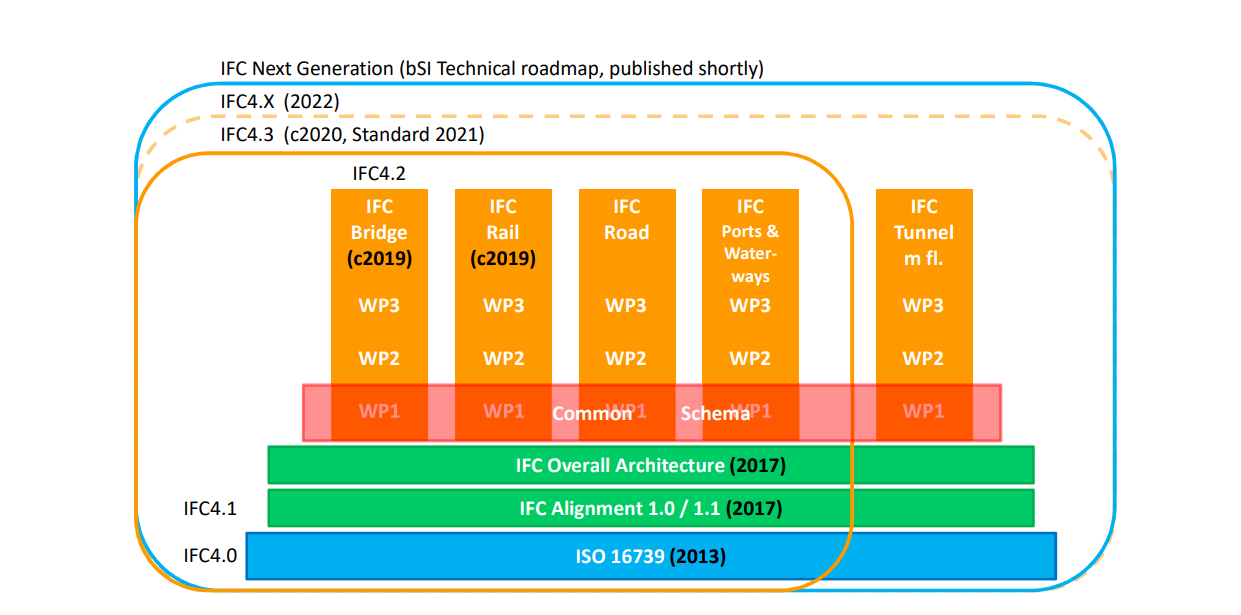
\includegraphics[width=0.7\textwidth]{IFC schema extensions}


Las especificaciones oficiales del estandard se pueden consultar en:
\begin{small}
\\ \url{https://technical.buildingsmart.org/standards/ifc/ifc-schema-specifications/}
\end{small}
Y se pueden obtener en formato digital en:
\begin{small}
\\ \url{https://github.com/buildingSMART/IfcDoc}
\end{small}

Algunos enlaces interesantes:
\begin{small}
\\ \url{https://www.buildingsmart.es/recursos/ifc-en-espa%C3%B1ol/classes/}
\\ \url{https://www.buildingsmart.es/recursos/ifc-en-espa%C3%B1ol/types/}
\\ \url{https://www.buildingsmart.es/recursos/ifc-en-espa%C3%B1ol/psets/}

\url{https://technical.buildingsmart.org/standards/ifc/ifc-tutorials/}

\end{small}

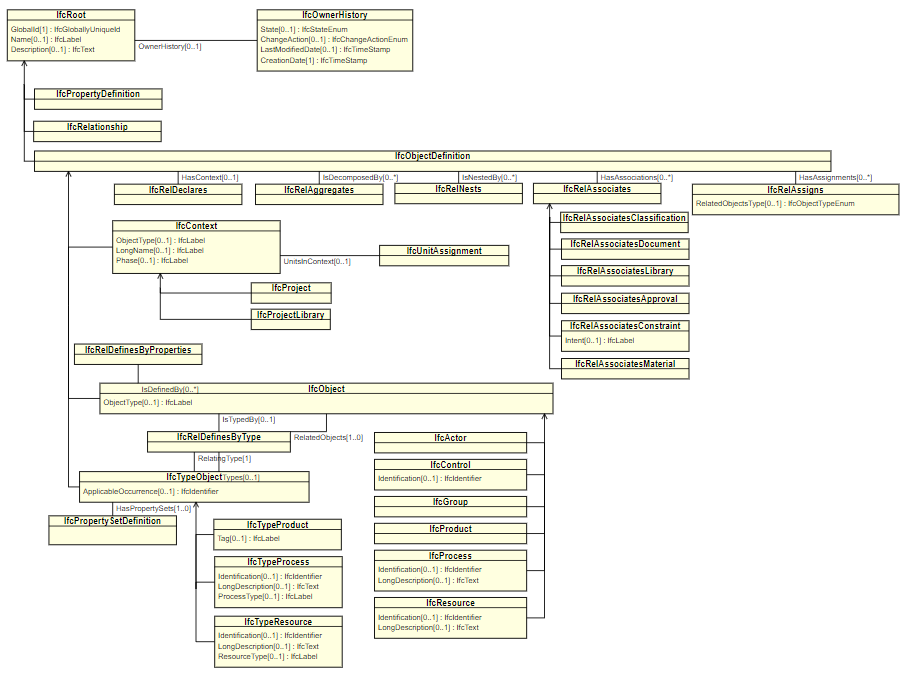
\includegraphics[width=0.8\textwidth]{principales relaciones entre los elementos principales}
\begin{flushright} 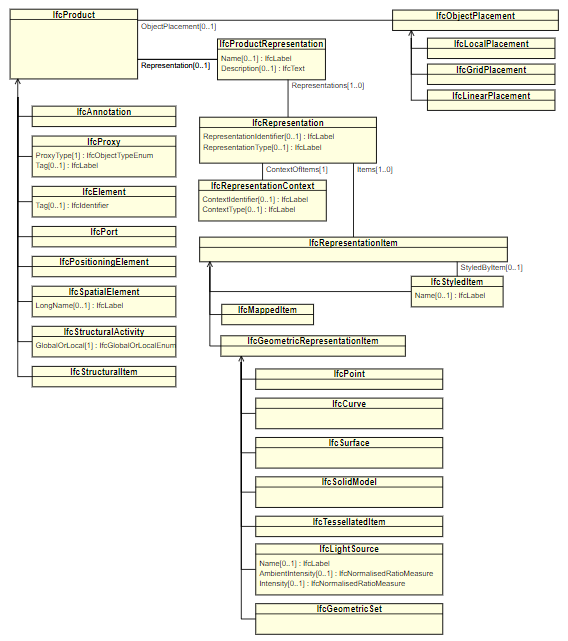
\includegraphics[width=0.5\textwidth]{principales relaciones de IfcProduct} \end{flushright} 


\chapter{Introducción: información que puede contener un modelo IFC}

\section{Estructuras espaciales y agrupaciones de entidades (IfcProject) (IfcSite) (IfcBuilding) (IfcWorkPlan) etc.}
\textbf{El proyecto} (IfcProject) recoge información general acerca del modelo. Por ejemplo: unidades de medida utilizadas, sistemas de coordenadas utilizados, geolocalización global, referencias a fuentes de clasificación externas,\ldots 

Sirve de ``contenedor'' para todas las demás entidades del modelo.

\url{https://standards.buildingsmart.org/IFC/RELEASE/IFC4/ADD2_TC1/HTML/link/ifcproject.htm}

\textbf{Un emplazamiento} (IfcSite) recoge información acerca de un área de terreno. Por ejemplo: referencias catastrales, puntos de referencia geográfica WSG84, puntos de elevación,\ldots

Sirve de ``contenedor'' para entidades tales como terreno, árboles, bosques, paradas de autobús, estanques, lagos, drenajes, señales, carreteras, puentes, edificios,\ldots. 

\url{https://standards.buildingsmart.org/IFC/RELEASE/IFC4/ADD2_TC1/HTML/link/ifcsite.htm}

\textbf{Un edificio} (IfcBuilding) recoge información acerca de un edificio o infraestructura. Por ejemplo: dirección postal, tipo de ocupación a la que se destina, área total construida, número de pisos, categorización mercantil, clasificación de eficiencia energética,\ldots

Sirve de ``contenedor'' para Productos.

\url{https://standards.buildingsmart.org/IFC/RELEASE/IFC4/ADD2_TC1/HTML/link/ifcbuilding.htm}

\textbf{Un plan de trabajo} (IfcWorkPlan) recoge información acerca de algo a realizar. Por ejemplo:  fecha prevista de inicio, fecha prevista de fin, el ``colchón'' de tiempo disponible para imprevistos, etc.   

Sirve de ``contenedor'' para entidades tales como calendarios, planificaciones, tareas, recursos utilizados,\ldots 

\url{https://standards.buildingsmart.org/IFC/RELEASE/IFC4/ADD2_TC1/HTML/link/ifcworkplan.htm}

\textbf{Etc}.

\section{Productos (IfcProduct)}
Un producto es una entidad física que se incorpora a la construcción. Por ejemplo: un muro, una ventana, un cuadro electrico, un conducto de ventilación,\ldots

\url{https://standards.buildingsmart.org/IFC/RELEASE/IFC4/ADD2_TC1/HTML/link/ifcproduct.htm}


\section{Recursos (IfcResource)}
Un recurso es una entidad que se utiliza en la construcción. Por ejemplo: materia prima, mano de obra, maquinaria, subcontratas, combustible,\ldots 

\url{https://standards.buildingsmart.org/IFC/RELEASE/IFC4/ADD2_TC1/HTML/link/ifcresource.htm}

 
\section{Procesos (IfcProcess)}
Un proceso es una actividad o evento, ordenado en el tiempo y relacionado secuencialmente con otros procesos.

Puede tener productos asignados a su entrada y productos asignados como su salida.

Puede tener recursos asignados como utilizados o consumidos durante el proceso.

\url{https://standards.buildingsmart.org/IFC/RELEASE/IFC4/ADD2_TC1/HTML/link/ifcprocess.htm}


\section{Controles (IfcControl)}
Un control es algo que restringe o modula la utilización de alguno de los productos, recursos o procesos. Por ejemplo: una normativa, un contrato, un pedido, una planificación, un permiso,\ldots

\url{https://standards.buildingsmart.org/IFC/RELEASE/IFC4/ADD2_TC1/HTML/link/ifccontrol.htm}


\section{Actores (IfcActor)}
Un actor es una persona u organización involucrada en el proyecto, en cualquiera de las etapas a lo largo de todo su ciclo de vida, Puede participar en un proceso, tener relación con algún objeto, conceder un permiso,\ldots

\url{https://standards.buildingsmart.org/IFC/RELEASE/IFC4/ADD2_TC1/HTML/link/ifcactor.htm}

\section{Grupos (IfcGroup)}
Un grupo es una colección lógica de entidades, simplemente porque nos conviene considerarlas así agrupadas para algún fin concreto.

\url{https://standards.buildingsmart.org/IFC/RELEASE/IFC4/ADD2_TC1/HTML/link/ifcgroup.htm}


\section{Un vistazo general a las entidades contempladas en las especificaciones IFC.}
Las especificaciones contienen esquemas detallados e información de uso de todas y cada una de las entidades que pueden aparecer dentro de un modelo IFC.
\\ \url{https://technical.buildingsmart.org/standards/ifc/ifc-schema-specifications/}
\\En esa página podemos encontrar enlaces a las distintas versiones de las especificaciones que se han ido sucediendo a lo largo del tiempo.

La versión oficial en estos momentos es la 4.0.2.1 (IFC4 ADD2 TC1) (ISO 16739-1:2018) 
\\ \url{https://standards.buildingsmart.org/IFC/RELEASE/IFC4/ADD2_TC1/HTML/}
\\Y la candidata a próxima versión es la 4.3.rc.2 (IFC4.3 RC2)
\\ \url{https://standards.buildingsmart.org/IFC/DEV/IFC4_3/RC2/HTML/}

Las especificaciones tienen varias secciones (numeradas) y varios apéndices (con letras).
\\ 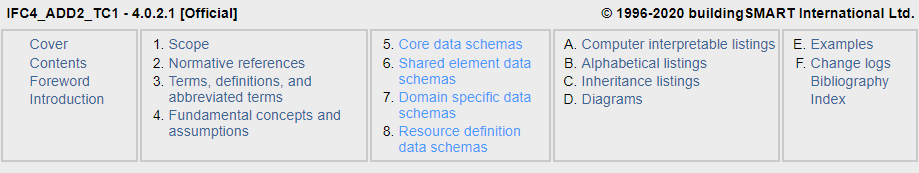
\includegraphics[width=\textwidth]{cabecera de las especificaciones}

Merece la pena echar primero un vistazo rápido a las secciones 6, 7 y 8. En estas secciones están las entidades más reconocibles.

En cada uno de los bloques de cada sección, las partes `Types' y `Entities' recogen las propias entidades en sí. Mientras que `Property Sets' (Pset\_) y `Quantity Sets' (Qto\_) recogen la información adicional que se puede asociar a esas entidades.

En la sección 5 están los esquemas de entidades ``especiales'', tales como las entidades que contienen otras entidades y las entidades que permiten expresar relaciones entre entidades.

\vspace{0.5cm}

Para hacerse una idea del propósito de una entidad concreta, merece mirar: la definición de la propia entidad (IfcXxxx), si tiene tipos de entidad que la especializan (IfcXxxxType), y si tiene alguna enumeración de tipos estandares predefinidos (IfcXxxxTypeEnum).

Dentro la página de cada entidad, merece mirar: su definición y propósito (Entity definition), sus atributos intrínsecos (Atribute definitions) y los atributos que hereda de otras entidades madre de las que deriva (Attibute inheritance).

\vspace{0.5cm}

nota: En cualquiera de las páginas, prácticamente todos los nombres de entidad (Ifc---) que aparezcan, aunque no estén en color azul-link, suelen ser un enlace a la página relativa a esa entidad. 

\subsection{sección `5. Core data schemas':}

\begin{description}
\item[entidades base (IfcKernel):] raiz (IfcRoot), objeto (IfcObject), proyecto (IfcProject), producto (IfcProduct), recurso (IfcResource), proceso (IfcProcess), conjunto de propiedades (IfcPropertySet), conjunto de cuantificadores (IfcQuantitySet), tipo (IfcRelDefines), relación (IfcRelationship), composición (IfcRelDeclares, IfcRelDecomposes), asignación (IfcRelAssigns), asociación (IfcRelAssociates), conexión (IfcRelConnects), etc.

\item[entidades base de `producto' (IfcProductExtension):] emplazamiento (IfcSite), edificio (IfcBuilding), sistema (IfcSystem), referencia de posicionamiento (IfcPositioningElement), rejilla de posicionamiento (IfcGrid), zona (IfcZone), area o volumen dedicado a algún propósito (IfcSpace), etc.
  
\item[entidades base de `proceso' (IfcProcessExtension):] evento (IfcEvent), tarea (IfcTask), procedimiento (IfcProcedure), calendario laboral (IfcWorkCalendar), planificación (IfcWorkPlan, IfcWorkSchedule), etc. 
\end{description}

\subsection{sección `6. Shared element data schemas':} 

\begin{description}
\item[Arquitectura (IfcSharedBldgElements):] viga (IfcBeam), columna (IfcColumn), muro (IfcWall), losa (IfcSlab), cubierta (IfcRoof), puerta (IfcDoor), ventana (IfcWindow), escalera (IfcStair), rampa (IfcRamp), etc.

\item[Distribución de sólidos, líquidos, gases, electricidad,\ldots (IfcSharedBldgServiceElements):] válvula o interruptor (IfcFlowController), tuberia o conducto (IfcFlowSegment), conector (IfcFlowFitting), depósito de almacenamiento (IfcFlowStorageDevice), boca de salida (IfcFlowTerminal), etc.

\item[Fijación entre objetos (IfcSharedComponentElements):] (IfcFastener), (IfcMechanicalFastener), etc.

\item[Bienes muebles (IfcSharedFacilitiesElements):] elemento de mobiliario (IfcFurniture), elemento de valor (IfcAsset), lista de elementos (IfcInventory), etc.

\item[Gestión administrativa (IfcSharedMgmtElements):] elemento de coste (IfcCostItem), presupuesto (IfcCostSchedule), solicitud (IfcActionRequest), pedido (IfcProjectOrder), autorización (IfcPermit), etc. 
\end{description}

\subsection{sección `7. Domain specific data schemas':}

\begin{description}
\item[Arquitectura (IfcArchitectureDomain):] marco de puerta (IfcDoorLiningProperties), hoja de puerta (IfcDoorPanelProperties), marco de ventana (IfcWindowLiningProperties), hoja de ventana (IfcWindowPanelProperties), etc.

\item[Domótica (IfcBuildingControlsDomain):] sensor (IfcSensor), avisador (IfcAlarm), medidor (IfcFlowInstrument), actuador (IfcActuator), etc.

\item[Participantes en la construcción (IfcConstructionMgmtDomain):] maquinaria o elemento auxiliar  que se utiliza o se consume (IfcConstructionEquipmentResource), elemento auxiliar que se construye para ser utilizado o consumido posteriormente (IfcConstructionProductResource),  materia prima que se consume (IfcConstructionMaterialResource), mano de obra (IfcLaborResource), recurso propio de la constructora (IfcCrewResource), recurso subcontratado (IfcSubContractResource), etc.

\item[Electricidad (IfcElectricalDomain):] cable (IfcCableSegment), conector (IfcCableFitting), canaleta (IfcCableCarrierSegment), conector de canaleta (IfcCableCarrierFitting), cuadro de distribución (IfcElectricDistributionBoard), caja de conexiones (IfcJunctionBox), enchufe (IfcOutlet), interruptor (IfcSwitchingDevice), equipo audiovisual (IfcAudioVisualAppliance), equipo de telecomunicaciones (IfcCommunicationsAppliance), lampara (IfcLamp), luminaria (IfcLightFixture), etc.

\item[Calefacción y aire acondicionado (IfcHvacDomain):] conducto (IfcDuctSegment), conector de conducto (IfcDuctFitting), tuberia (IfcPipeSegment), conector de tuberia (IfcPipeFitting), bomba (IfcPump), válvula (IfcValve), ventilador (IfcFan), calentador (IfcBoiler), enfriador (IfcChiller), caldera (IfcBurner), condensador (IfcCondenser), evaporador (IfcEvaporator), humidificador (IfcHumidifier), etc.

\item[Desagües y sistemas anti-incendios (IfcPlumbingFireProtectionDomain):] fregadero (IfcSanitaryTerminal), desagüe (IfcWasteTerminal), rejilla de aireación (IfcStackTerminal), rejilla de retención de sólidos (IfcInterceptor), rociador (IfcFireSuppresionTerminal), etc.

\item[Cálculo estructural (IfcStructuralAnalysisDomain):] elemento que soporta carga (IfcStructuralItem, IfcStructuralCurveMember, IfcStructuralSurfaceMember), elemento que transmite carga (IfcStructuralConnection), caso de carga (IfcStructuralLoadGroup), caso de uso (IfcStructuralLoadCase), carga aplicada (IfcStructuralAction), carga puntual (IfcStructuralPointAction), carga distribuida (IfcLinearAction, IfcStructuralCurveAction, IfcSurfaceAction), grupo de resultados (IfcStructuralResultGroup), reacción resultante (IfcStructuralReaction, IfcStructuralCurveReaction, IfcStructuralSurfaceReaction), etc.

\item[Elementos estructurales (IfcStructuralElementsDomain):] zapata (IfcFooting), pilote (IfcPile), ferralla (IfcReinforcingBar), tendón para pretensado (IfcTendon), etc. 
\end{description}
 
\subsection{sección `8. Resource definition data schemas':}

\begin{description}
\item[Actores (IfcActorResource):] organización (IfcOrganization), persona (IfcPerson), dirección postal (IfcPostalAddress), telefono/fax/correo-e (IfcTelecomAddress), papel  desempeñado en (IfcActorRole), etc.

\item[Autorizaciones (IfcApprovalResource):] autorización (IfcApproval), otras autorizaciones relacionadas con esta (IfcApprovalRelationship), recursos relacionados con esta autorización (IfcResourceApprovalRelationship).

\item[Condiciones (IfcConstraintResource):] límite (IfcConstraint), indicador (IfcMetric), objetivo (IfcObjective), referencia (IfcReference), recursos relacionados con esta condición (IfcResourceConstraintRelationship), forma de aplicación (IfcBenchmarkEnum), nivel de obligatoriedad (IfcConstraintEnum), etc.

\item[Costes (IfcCostResource):] cantidad de dinero (IfcCostValue), cantidad calculada (IfcAppliedValue), cotización de divisa (IfcCurrencyRelationship), etc.

\item[Fechas y horas (IfcDateTimeResource):] fecha (IfcDate), hora (IfcTime), intervalo (IfcLagTime), datos temporales para definir calendarios de trabajo (IfcWorkTime), datos temporales relativos a una tarea (IfcTaskTime), serie temporal de datos (IfcRegularTimeSeries) (IfcIrregularTimeSeries), momento en que ha sucedido o va a suceder algo (IfcEventTime), etc.

\item[Referencias externas (IfcExternalReferenceResource):] URI (IfcDocumentReference), metadatos bibliograficos (IfcDocumentInformation), otros documentos relacionados con este (IfcDocumentInformationRelationship), nivel de confidencialidad (IfcDocumentConfidentialityEnum), estado de redacción (IfcDocumentStatusEnum), idioma en que está escrito (IfcLanguageId), sistema de clasificación (IfcClassification), clave de clasificación (IfcClassificationReference), etc.

\item[Posicionamiento y orientación  (IfcGeometricConstraintResource):]  (IfcAligment2DHorizontal), (IfcAligment2DVertical), (IfcAligmentCurve), (IfcGridAxis), (IfcObjectPlacement),(IfcLinearPlacement), (IfcGridPlacement), (IfcConnectionGeometry), etc.

\item[Formas geométricas (IfcGeometricModelResource):] caja contenedora (IfcBoundingBox), nube de puntos (IfcCartesianPointList), paralelepípedo (IfcBlock), esfera (IfcSphere), cilindro (IfcRightCircularCylinder), sólido de revolución (IfcRevolvedAreaSolid), sólido extruido (IfcSweptAreaSolid), representación por caras, aristas y vértices  (IfcAdvancedBrep), representación por caras planas (IfcFacetedBrep), etc.

\item[Recursos utilizados para representar geometria (IfcGeometryResource):] punto unidimensional (IfcPoint, IfcCartesianPoint, IfcPointOnCurve, IfcPointOnSurface), curva bidimensional (IfcLine, IfcCurve, IfcPolyline, IfcCircle, IfcEllipse, IfcConic, IfcRationalBSplineCurve), superficie tridimensional (IfcSurface, IfcSphericalSurface, IfcToroidalSurface, IfcSurfaceOfRevolution, IfcSweptSurface, IfcRationalBSplineSurface), vector (IfcVector), productos entre vectores (IfcDotProduct, IfcCrossProduct), referencia de ubicación espacial tridimensional (IfcAxis1Placement, IfcAxis2Placement3D, IfcAxis2Placement3D), comparador de posiciones (IfcSameCartesianPoint), comparador de direcciones (IfcSameDirection), etc.

\item[Materiales, substancias de las cuales está hecho algo (IfcMaterialResource):] material (IfcMaterial), cada una de las partes de distinto material en un composite (IfcMaterialConstituent), cada una de las capas de distinto material en un material multicapa (IfcMaterialLayer), propiedades de un material (Pset\_MaterialConcrete, Pset\_MaterialSteel, Pset\_MaterialWood, Pset\_MaterialWater, Pset\_MaterialMechanical, Pset\_MaterialThermal, etc.), etc.

\item[Unidades de medida (IfcMeasureResource):] longitud (IfcLengtMeasure), área (IfcAreaMeasure), volumen (IfcVolumeMeasure), ángulo sólido (IfcSolidAngleMeasure), masa (IfcMassMeasure), fuerza (IfcForceMeasure), momento de inercia (IfcMomentOfInertiaMeasure), tiempo (IfcTimeMeasure), aceleración (IfcAccelerationMeasure), voltaje (IfcElectricVoltageMeasure), resistencia (IfcElectricResistanceMeasure), intensidad (IfcElectricCurrentMeasure), luminancia (IfcIlluminanceMeasure), intensidad luminosa (IfcLuminousIntensityMeasure), flujo lumínico (IfcLuminousFluxMeasure), dinero (IfcMonetaryMeasure), peso molecular (IfcMolecularWeightMeasure), etc.

\item[Estilos de representación (IfcPresentationAppearanceResource):] estilo de texto (IfcFontStyle), variantes de texto (IfcFontStyle, IfcFontVariant, IfcFontWeight), tipografia (IfcTextFontName), color (IfcColour, IfcColourRgb, etc.), textura (IfcPixelTexture, IfcSurfaceTexture, etc.), renderizado (IfcSurfaceStyleLighting, IfcSurfaceStyleRefraction, IfcSurfaceStyleShading, etc.), etc.  

\item[Anotaciones (IfcPresentationDefinitionResource):] areas reservadas para texto (IfcAnnotationFillArea) (IfcPlanarBox), texto (IfcTextLiteral), etc.

\item[Capas e iluminación (IfcPresentationOrganizationResource):] capas CAD (IfcPresentationLayerAssignment), visibilidad/bloqueo (IfcPresentationLayerWithStyle), fuente de luz (IfcLightSource, IfcLightSourceAmbient, IfcLightSourceDirectional, IfcLightSourceGoniometric, IfcLightSourcePositional, IfcLightSourceSpot), etc.   

\item[Perfiles y secciones (IfcProfileResource):] perfileria (IfcProfileProperties, IfcProfileTypeEnum, IfcProfileDef, IfcCircleProfileDef, IfcEllipseProfileDef, IfcLShapeProfileDef, IfcIShapeProfileDef, IfcRectangleProfileDef, etc.), ferralla (IfcReinforcementBarProperties, IfcReinforcementBarRoleEnum, IfcReinforcementBarSurfaceEnum, etc.), etc.

\item[Propiedades (IfcPropertyResource):] (IfcPropertySingleValue) (IfcPropertyListValue) (IfcPropertyTableValue) (IfcPropertyEnumeratedValue) etc. 

\item[Cuantificadores (IfcQuantityResource):] (IfcQuantityCount) (IfcQuantityLength) (IfcQuantityArea) (IfcQuantityVolume) (IfcQuantityWeight) (IfcQuantityTime) etc.

\item[Representaciones gráficas (IfcRepresentationResource):] sistema de referencia (IfcCoordinateReferenceSystem), representacion geomética (IfcShapeRepresentation), representación topológica (IfcTopologyRepresentation), etc. 

\item[Cálculo estructural (IfcStructuralLoadResource):] restricción (IfcBoundaryNodeCondition, IfcBoundaryEdgeCondition, IfcBoundaryFaceCondition, etc.), holgura (IfcSlippageConnectionCondition, IfcFailureConnectionCondition, IfcStructuralConnectionCondition), carga/reacción (IfcStructuralLoadForce, IfcStructuralLoadLinearForce, IfcStructuralLoadPlanarForce, etc.), desplazamiento (IfcStructuralLoadSingleDisplacement), dilatacion (IfcStructuralLoadTemperature), etc. 

\item[Representación topológica (IfcTopologyResource):] vértice (IfcVertex), arista (IfcEdge) (IfcOrientedEdge), cara (IfcFace), cadena de bordes (IfcPath) (IfcLoop), etc.

\item[Control de cambios (IfcUtilityResource):] identificador único GUID (IfcGloballyUniqueId), sincambios/modificado/añadido/eliminado (IfcChangeActionEnum), bloqueado/sololectura/lecturaescritura (IfcStateEnum), tabla (IfcTable), fila (IfcTableRow), columna (IfcTableColumn), etc.

\end{description}


\begin{minipage}{\textwidth}

\subsection{Comentarios sobre las demás secciones de las especificaciones}
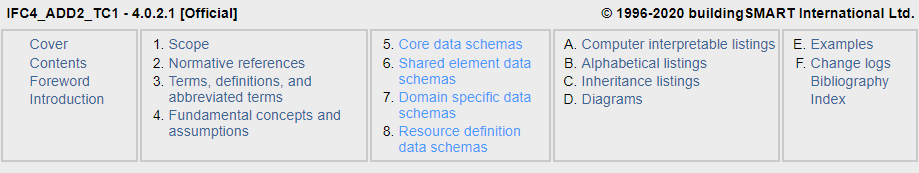
\includegraphics[width=\textwidth]{cabecera de las especificaciones}

\vspace{0.5cm}

Para una idea general de cómo se usan algunas de las distintas entidades, es conveniente echar un vistazo a los ejemplos del anexo E.

\vspace{0.5cm}

Para una referencia rápida de cómo se relacionan las entidades es útil acudir a los diagramas del anexo D: agrupados según esquemas, en D.1 ; o por orden alfabético, en D.2

\vspace{0.5cm}

Para buscar una entidad concreta y las relacionadas directamente con ella, acudir al índice (Index).

\vspace{0.5cm}

Después de familiarizarse un poco con la variedad de entidades disponibles, merece echar un vistazo a la sección `4. Fundamental concepts and assumptions.'

\end{minipage}



\chapter{Introducción: estructura interna de la información en el modelo}


\section{Los ``\textbf{contenedores}'' de entidades}

\subsection{contexto general}
\textbf{El proyecto (IfcProject)} es LA agrupación de todas las demás entidades del modelo.
\\ \url{https://standards.buildingsmart.org/IFC/RELEASE/IFC4/ADD2_TC1/HTML/schema/templates/project-context.htm}
\\ 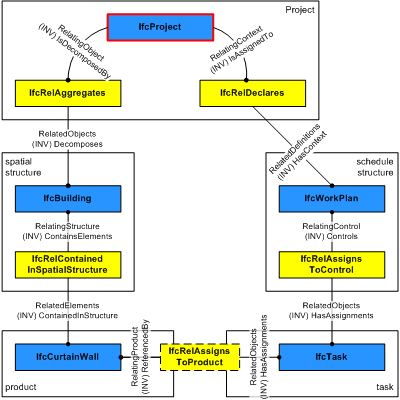
\includegraphics[width=0.5\textwidth]{principales relaciones de IfcProject}
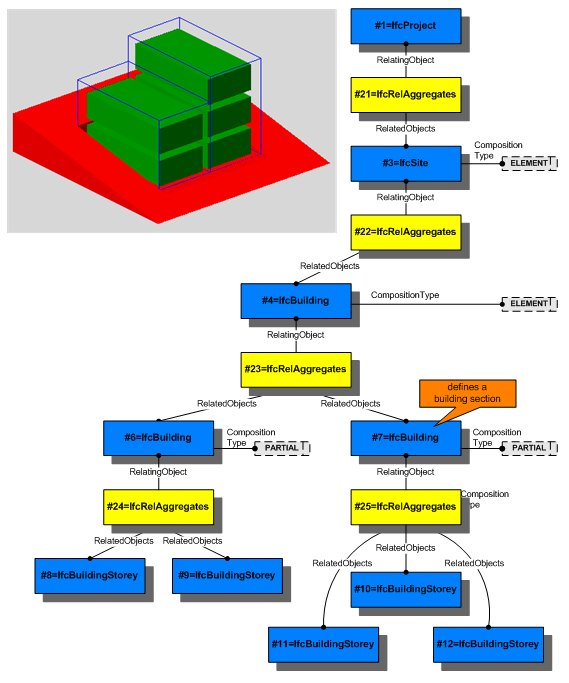
\includegraphics[width=0.5\textwidth]{principales relaciones de IfcSpacialStructureElement}

\subsection{contexto espacial}
\textbf{Un emplazamiento (IfcSite)} es una agrupación de objetos dentro de un área de terreno donde se va a trabajar.
\\ \url{https://standards.buildingsmart.org/IFC/RELEASE/IFC4/ADD2_TC1/HTML/link/ifcsite.htm}
\\ 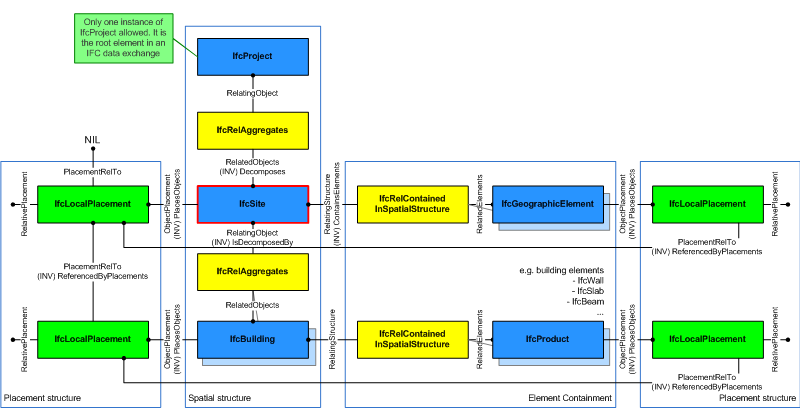
\includegraphics[width=\textwidth]{principales relaciones de IfcSite}

\textbf{Un edificio (IfcBuilding)} es una agrupación de objetos dentro de un edificio o infraestructura.
\\ \url{https://standards.buildingsmart.org/IFC/RELEASE/IFC4/ADD2_TC1/HTML/link/ifcbuilding.htm}
\\ 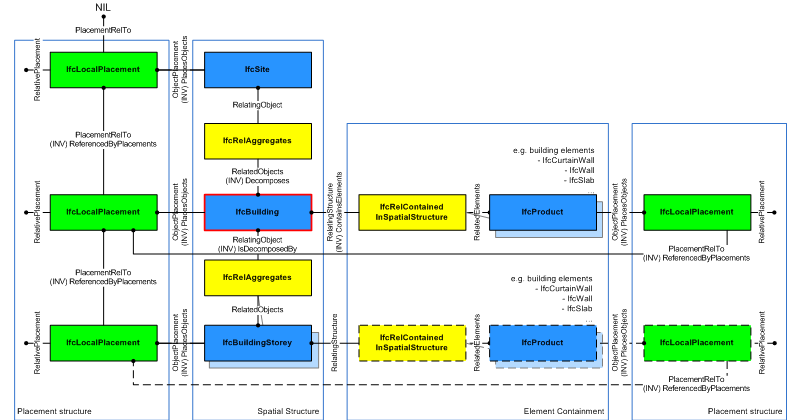
\includegraphics[width=\textwidth]{principales relaciones de IfcBuilding}

\vspace{1cm}
 
\textbf{Una planta (IfcBuildingStorey)} es una agrupación de objetos dentro de una extensión horizontal a una determinada altura.
\\ \url{https://standards.buildingsmart.org/IFC/RELEASE/IFC4/ADD2_TC1/HTML/link/ifcbuildingstorey.htm}
\\ 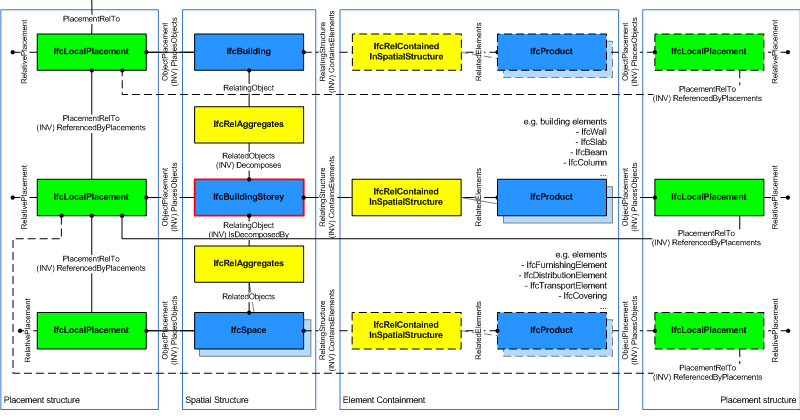
\includegraphics[width=\textwidth]{principales relaciones de IfcBuildingStorey}

\subsection{contexto temporal}
\textbf{Un plan de trabajo (IfcWorkPlan)} es una agrupación de entidades tales como calendarios, planificaciones, tareas, recursos utilizados,\ldots 
\\ \url{https://standards.buildingsmart.org/IFC/RELEASE/IFC4/ADD2_TC1/HTML/link/ifcworkplan.htm}
\\ 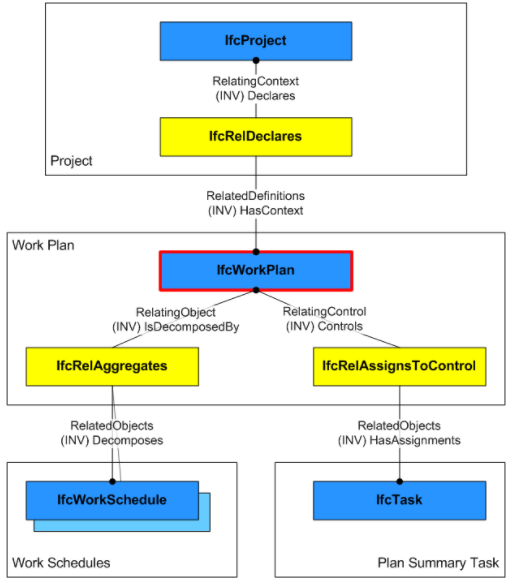
\includegraphics[width=0.6\textwidth]{principales relaciones de IfcWorkPlan}

\vspace{1cm}

\textbf{Un calendario de trabajos (IfcWorkSchedule)} es una agrupación de una secuencia de tareas dentro de un plan de trabajo.
\\ \url{https://standards.buildingsmart.org/IFC/RELEASE/IFC4/ADD2_TC1/HTML/link/ifcworkschedule.htm}
\\ 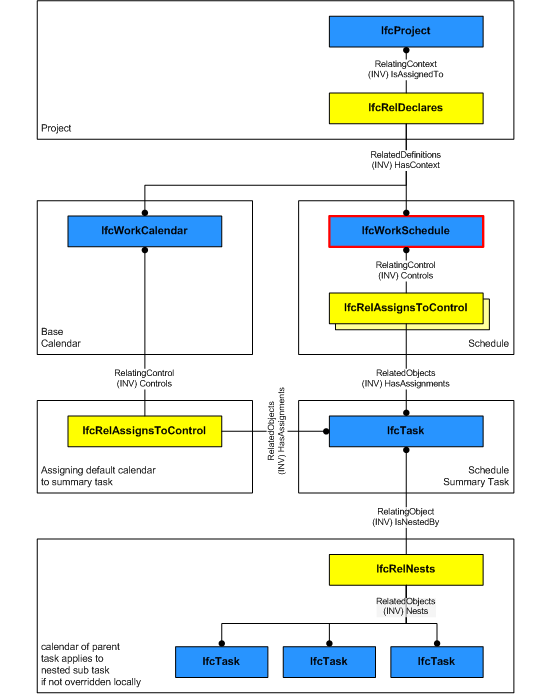
\includegraphics[width=0.6\textwidth]{principales relaciones de IfcWorkSchedule}



\subsection{contexto funcional}
\textbf{Un sistema (IfcBuidingSystem)} es una agrupación de objetos relacionados con una determinada una funcionalidad  dentro de un edificio o infraestructura.
\\ \url{https://standards.buildingsmart.org/IFC/RELEASE/IFC4/ADD2_TC1/HTML/link/ifcbuildingsystem.htm}

IfcBuildingSystemTypeEnum
\\ 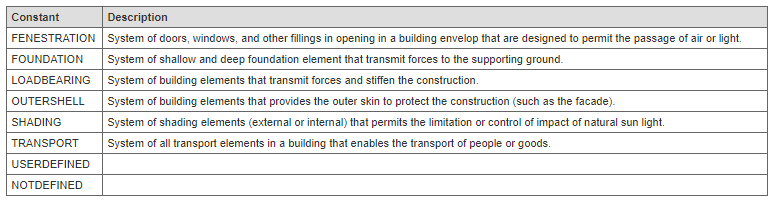
\includegraphics[width=\textwidth]{Definicion de IfcBuildingSystemTypeEnum}

\textbf{Un modelo de cálculo estructural (IfcStructuralAnalysisModel)} es una agrupación de elementos relacionados con un determinado cálculo: modelo a calcular, restricciones y cargas aplicadas, resultados obtenidos,\ldots 
\\ \url{https://standards.buildingsmart.org/IFC/RELEASE/IFC4/ADD2_TC1/HTML/link/ifcstructuralanalysismodel.htm}



\section{Las \textbf{entidades} (IfcXxxx) (IfcXxxxType)}

Para hacerse una idea del propósito de una entidad concreta, merece mirar: la definición de la propia entidad (IfcXxxx), si tiene tipos de entidad que la especializan (IfcXxxxType), y si tiene alguna enumeración de tipos estándares predefinidos (IfcXxxxTypeEnum).

Dentro la página de cada entidad, merece mirar: su definición y propósito (Entity definition), sus atributos (Atribute definitions) y los atributos que hereda de otras entidades madre de las que deriva (Attibute inheritance).


\subsection{Algunos ejemplos:}

\subsubsection{Una persona:}
IfcPerson
\\ \url{https://standards.buildingsmart.org/IFC/RELEASE/IFC4/ADD2_TC1/HTML/link/ifcperson.htm}
\\ 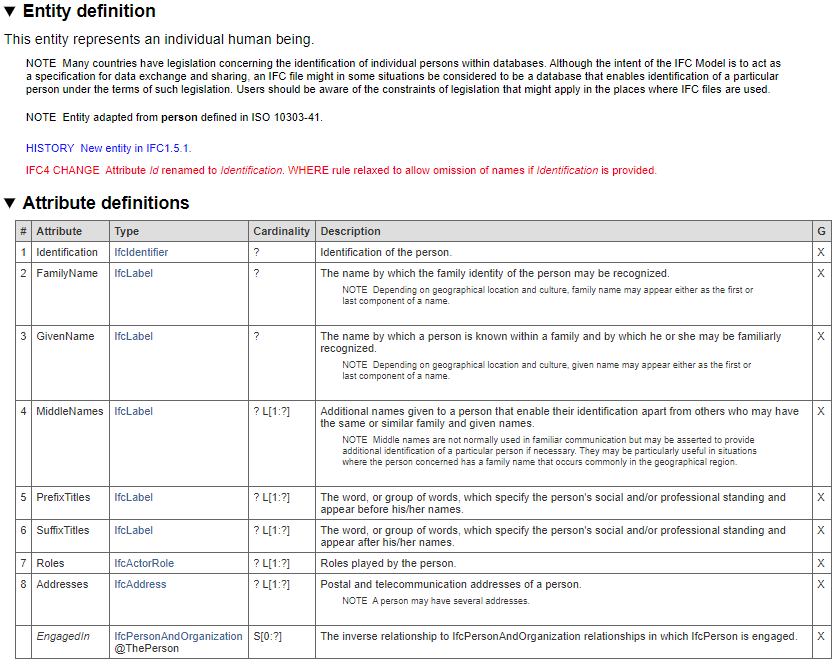
\includegraphics[width=\textwidth]{Definicion de IfcPerson}

\subsubsection{Una materia prima:}
IfcConstructionMaterialResource
\\ \url{https://standards.buildingsmart.org/IFC/RELEASE/IFC4/ADD2_TC1/HTML/link/ifcconstructionmaterialresource.htm}
\\ 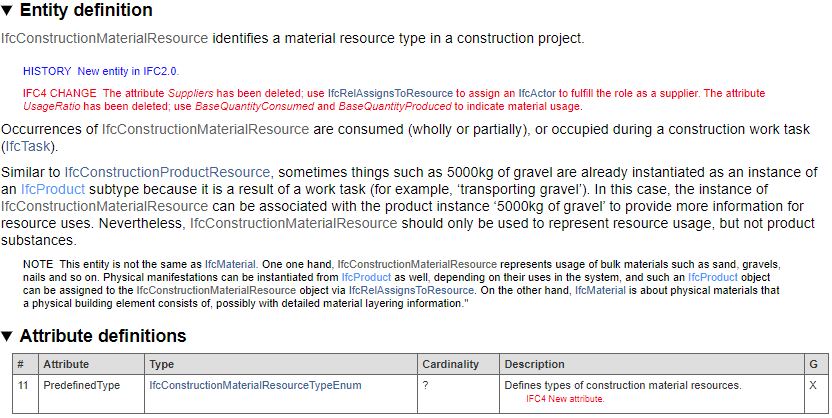
\includegraphics[width=\textwidth]{Definicion de IfcConstructionMaterialResource}

IfcConstructionMaterialResourceTypeEnum
\\ \url{https://standards.buildingsmart.org/IFC/RELEASE/IFC4/ADD2_TC1/HTML/link/ifcconstructionmaterialresourcetypeenum.htm}
\\ 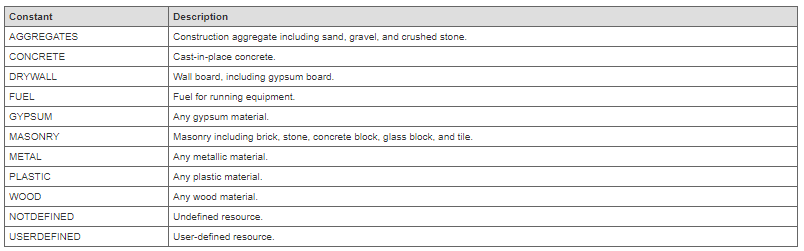
\includegraphics[width=\textwidth]{Definicion de IfcConstructionMaterialResourceTypeEnum}

\subsubsection{Un muro:}
IfcWall
\\ \url{https://standards.buildingsmart.org/IFC/RELEASE/IFC4/ADD2_TC1/HTML/link/ifcwall.htm}
\\IfcWallStandardCase
\\ \url{https://standards.buildingsmart.org/IFC/RELEASE/IFC4/ADD2_TC1/HTML/link/ifcwallstandardcase.htm}
\\IfcWallElementedCase
\\ \url{https://standards.buildingsmart.org/IFC/RELEASE/IFC4/ADD2_TC1/HTML/link/ifcwallelementedcase.htm}
\\ 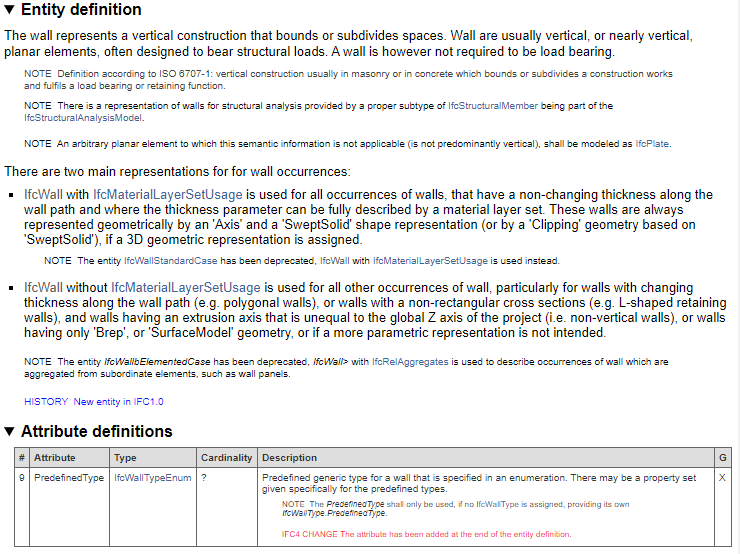
\includegraphics[width=\textwidth]{Definicion de IfcWall}

IfcWallTypeEnum
\\ \url{https://standards.buildingsmart.org/IFC/RELEASE/IFC4/ADD2_TC1/HTML/link/ifcwalltypeenum.htm}
\\ 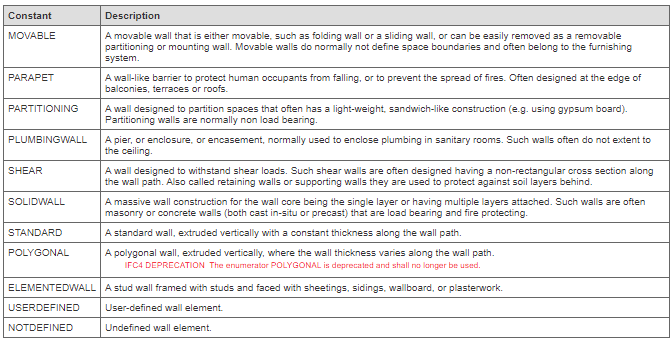
\includegraphics[width=\textwidth]{Definicion de IfcWallTypeEnum}



\section{Los \textbf{atributos} de las entidades, información intrínseca a la entidad}
\url{https://standards.buildingsmart.org/IFC/RELEASE/IFC4/ADD2_TC1/HTML/schema/templates/object-attributes.htm}

En la definición de cada entidad se puede encontrar una relación de los datos intrínsecos que la caracterizan: sus atributos.

Por ejemplo:
\begin{itemize}

\item Para un emplazamiento (IfcSite):
\\ 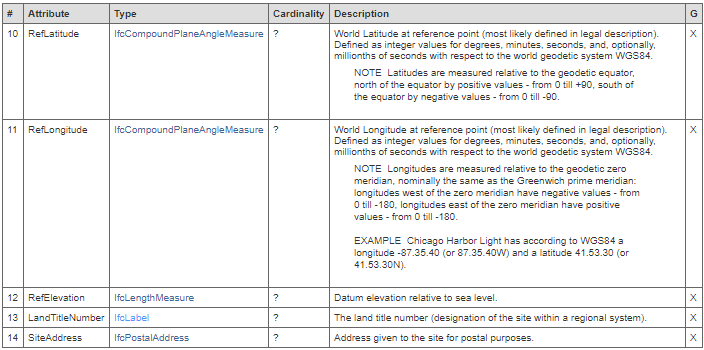
\includegraphics[width=\textwidth]{atributos de IfcSite}

\begin{minipage}{\textwidth}
\item Para un muro (IfcWall):
\\ 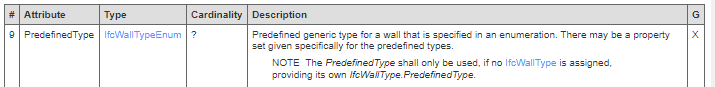
\includegraphics[width=\textwidth]{atributos de IfcWall}
\\ (IfcWallStandardCase)
\\ 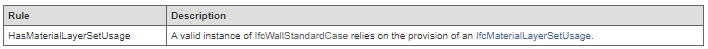
\includegraphics[width=\textwidth]{atributos de IfcWallStandardCase}
\\ (IfcWallElementedCase)
\\ 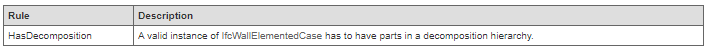
\includegraphics[width=\textwidth]{atributos de IfcWallElementedCase}
\end{minipage}

\item Para una empresa (IfcOrganization):
\\ 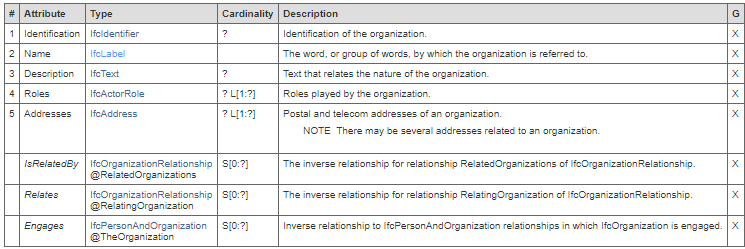
\includegraphics[width=\textwidth]{atributos de IfcOrganization}

\end{itemize}


\subsection{Herencia de atributos}
Una entidad tiene unos atributos propios de su definición. Pero también puede heredar otros atributos de sus ancestros.

Por ejemplo, un muro (IfcWall) tiene esta jerarquia de herencias:
\\ 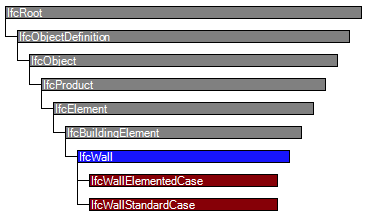
\includegraphics[scale=.7]{jerarquia de IfcWall}

Lo que significa que, además de su propios atributos como muro (IfcWall):
\\ 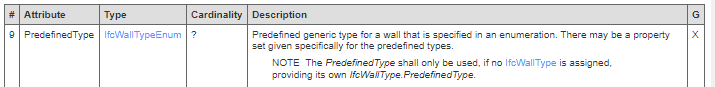
\includegraphics[width=.7\textwidth]{atributos de IfcWall}

, tiene también estos otros atributos:
\begin{itemize}
\item heredados de IfcRoot:
\\ 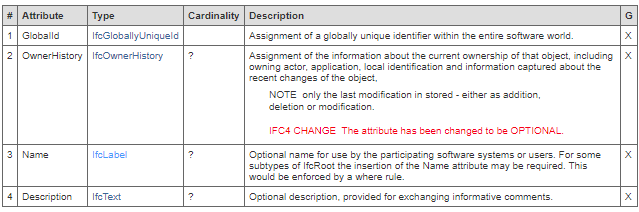
\includegraphics[width=.7\textwidth]{atributos de IfcRoot}

\item heredados de IfcObjectDefinition:
\\ 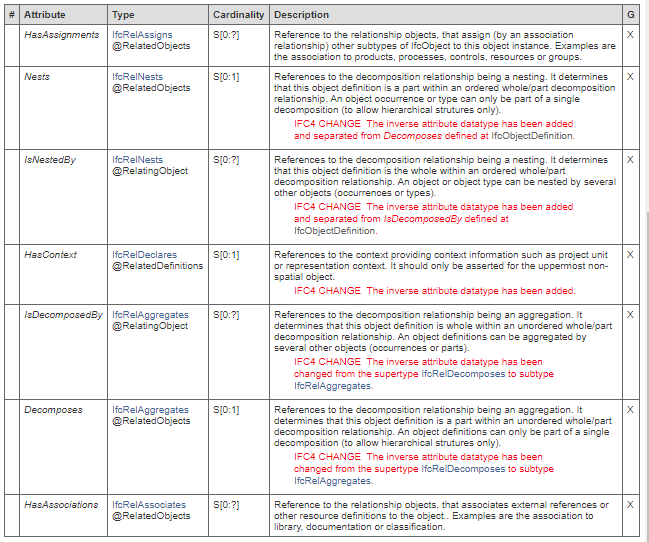
\includegraphics[width=.7\textwidth]{atributos de IfcObjectDefinition}

\item heredados de IfcObject:
\\ 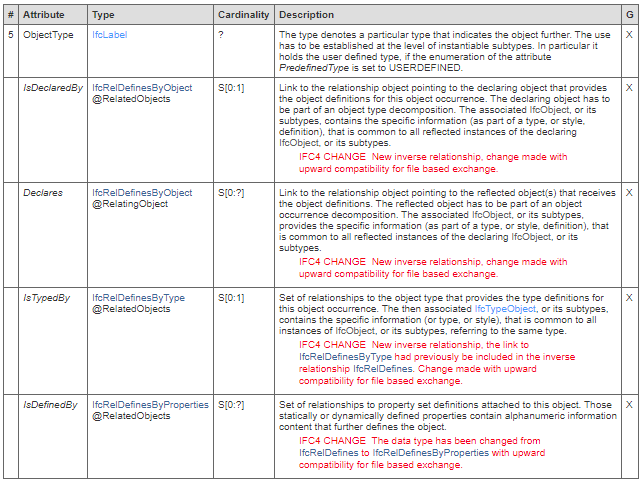
\includegraphics[width=.8\textwidth]{atributos de IfcObject}

\item heredados de IfcProduct:
\\ 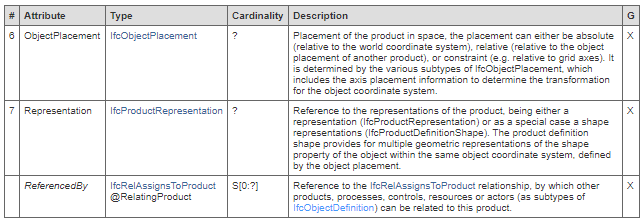
\includegraphics[width=.8\textwidth]{atributos de IfcProduct}

\item heredados de IfcElement:
\\ 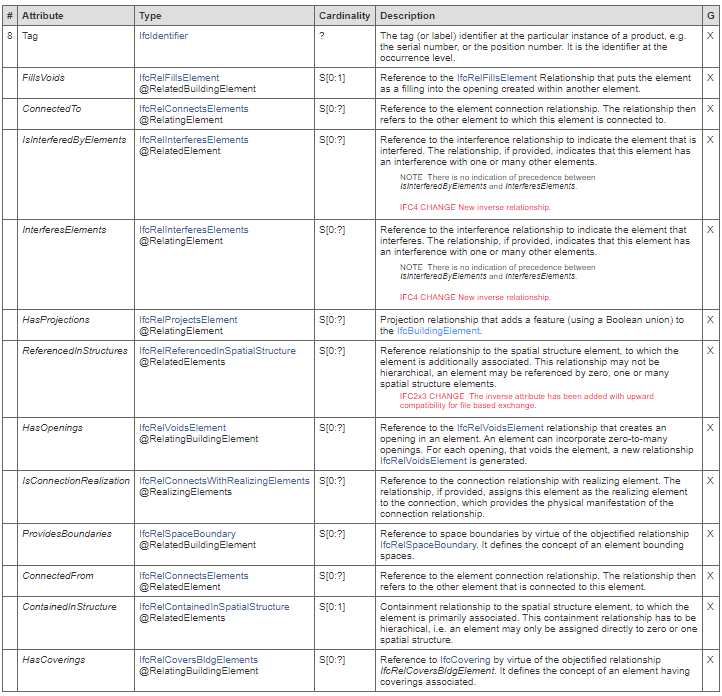
\includegraphics[width=.8\textwidth]{atributos de IfcElement}

\item heredados de IfcBuildingElement:
\\ninguno
\end{itemize}



\section{Las \textbf{propiedades} (PSet\_ ) y los \textbf{cuantificadores} (Qto\_ ), información adicional acerca de la entidad}

Una entidad puede tener asociadas una serie de conjuntos de propiedades (PSet\_) con datos acerca de ella y una serie de conjuntos de magnitudes (Qto\_) que se pueden medir sobre ella.


\subsection{Por ejemplo, para un muro:}
\begin{description}

\item[Pset\_WallCommon] Datos principales $\rightarrow$ referencia identificadora dentro del proyecto (Reference), es nuevo/existente/ademoler/temporal\ldots (Status), es un muro de carga (LoadBearing), nivel de aislamiento acústico (AcousticRating), nivel de resistencia al fuego (FireRating), etc.
\\ \url{https://standards.buildingsmart.org/IFC/RELEASE/IFC4/ADD2_TC1/HTML/link/pset_wallcommon.htm}

\item[Qto\_WallBaseQuantities] Magnitudes principales $\rightarrow$ longitud (Length), anchura (Width), altura (Height), área ocupada en el suelo (GrossFootprintArea, NetFootprintArea), área ocupada de forma vertical (GrossSideArea, NetSideArea), volumen ocupado (GrossVolume, NetVolume), peso (GrossWeight, NetWeight).
\\ \url{https://standards.buildingsmart.org/IFC/RELEASE/IFC4/ADD2_TC1/HTML/link/qto_wallbasequantities.htm}

\item[Pset\_ConcreteElementGeneral] Datos relativos a un elemento hecho de cemento $\rightarrow$ método constructivo (ConstructionMethod), clase estructural (StructuralClass), porcentaje de armados (ReinforcementVolumeRatio), etc.
\\ \url{https://standards.buildingsmart.org/IFC/RELEASE/IFC4/ADD2_TC1/HTML/link/pset_concreteelementgeneral.htm}

\item[Pset\_PrecastConcreteElementFabrication] Datos relativos a un elemento prefabricado $\rightarrow$ tipo (TypeDesignator), lote de producción (productionLotId), número de serie (SeriaNumber), número de pieza (PieceMark), fecha de fabricación (ActualProductionDate), fecha de puesta en obra (ActualErectionDate), etc.
\\ \url{https://standards.buildingsmart.org/IFC/RELEASE/IFC4/ADD2_TC1/HTML/link/pset_precastconcreteelementfabrication.htm}

\item[Pset\_PrecastConcreteElementGeneral] Datos relativos a un prefabricado de cemento $\rightarrow$ grado de curación mínimo para que el elemento pueda ser izado (LiftingStrength), grado de curación mínimo para poder relajar los tendones de pretensado (TendonRelaxation), instrucciones para sujetar el elemento durante el transporte (SupportDuringTransportDescription), documentación adicional con instrucciones para el transporte  (SupportDuringTransportDocReference), instrucciones para proteger las partes huecas durante el transporte y almacenamiento (HollowCorePlugging), etc.
\\ \url{https://standards.buildingsmart.org/IFC/RELEASE/IFC4/ADD2_TC1/HTML/link/pset_precastconcreteelementgeneral.htm}

\item[Pset\_ReinforcementBarPitchOfWall] Datos relativos a los armados $\rightarrow$ descripción (Description), referencia a un tipo de armado específico dentro del contexto del proyecto (Reference), tipo de colocación de las barras de armado (BarAllocationType), etc.
\\ \url{https://standards.buildingsmart.org/IFC/RELEASE/IFC4/ADD2_TC1/HTML/link/pset_reinforcementbarpitchofwall.htm}

\item[Pset\_EnvironmentalImpactIndicators] Datos relativos al impacto medioambiental, según norma \begin{footnotesize} ISO21930:2007\end{footnotesize} $\rightarrow$ fase del ciclo de vida para la cual son validos estos datos (LifeCyclePhase), años de vida media esperada (ExpectedServiceLife), consumo unitario de agua (WaterConsumptionPerUnit), residuos peligrosos producidos por unidad (HazardousWastePerUnit), residuos normales producidos por unidad (NonHazardousWastePerUnit), tasa de CO$_{2}$ producido por unidad (ClimateChangePerUnit), etc.
\\ \url{https://standards.buildingsmart.org/IFC/RELEASE/IFC4/ADD2_TC1/HTML/link/pset_environmentalimpactindicators.htm}

\item[Pset\_EnvironmentalImpactValues] Datos sobre costes medioambientales $\rightarrow$ consumo de agua (WaterConsumption), consumo de energia (TotalPrimaryEnergyConsuption), residuos peligrosos generados (HazardousWaste), residuos generados (NonHazardousWaste), residuos inertes (InertWaste), residuos radioactivos (RadioactiveWaste), etc.
\\ \url{https://standards.buildingsmart.org/IFC/RELEASE/IFC4/ADD2_TC1/HTML/link/pset_environmentalimpactvalues.htm}

\item[Pset\_Condition] Revisión del estado de la construcción $\rightarrow$ fecha de la inspección (AssessmentDate), resumen de la inspección (AssessmentCondition), descrición detallada de la inspección (AssessmentDescription).
\\ \url{https://standards.buildingsmart.org/IFC/RELEASE/IFC4/ADD2_TC1/HTML/link/pset_condition.htm}

\item[Pset\_ManufacturerOccurrence] Datos del elemento $\rightarrow$ fecha de adquisición (AcquisitionDate), código de barras (BarCode), número de serie (SerialNumber), referencia de lote (BatchReference), etc.
\\ \url{https://standards.buildingsmart.org/IFC/RELEASE/IFC4/ADD2_TC1/HTML/link/pset_manufactureroccurrence.htm}

\item[Pset\_ManufacturerTypeInformation] Datos del fabricante  $\rightarrow$ identificador GS1 (GlobalTradeItemNumber), código de artículo (ArticleNumber), nombre del fabricante (Manufacturer), lugar de fabricación (AssemblyPlace), etc.
\\ \url{https://standards.buildingsmart.org/IFC/RELEASE/IFC4/ADD2_TC1/HTML/link/pset_manufacturertypeinformation.htm}

\item[Pset\_ServiceLife] Datos de servicio $\rightarrow$ vida media esperada (ServiceLifeDuration), tiempo medio entre fallos (MeanTimeBetweenFailure).
\\ \url{https://standards.buildingsmart.org/IFC/RELEASE/IFC4/ADD2_TC1/HTML/link/pset_servicelife.htm}

\item[Pset\_Warranty] Datos de garatia $\rightarrow$ número de póliza (WarrantyIdentifier), fecha de inicio (WarrantyStartDate), fecha de expiración (WarrantyEndDate), ¿es una garantia extendida? (IsExtendedWarranty), periodo de garantia (WarrantyPeriod),  aspectos cubiertos  (WarrantyContent), aspectos excluidos (Exclusions), contacto al que recurrir en caso de incidente (PointOfContact).
\\ \url{https://standards.buildingsmart.org/IFC/RELEASE/IFC4/ADD2_TC1/HTML/link/pset_warranty.htm}

\end{description}



\section{Las \textbf{relaciones} entre entidades}
Un modelo IFC es una estructura entrelazada donde unas entidades están relacionadas con otras de muy diversas maneras.

\subsection{Posicionamiento relativo}
Ubicación y orientación de una entidad física dentro del modelo con relación a otras entidades del mismo.
\\ \url{https://standards.buildingsmart.org/IFC/RELEASE/IFC4/ADD2_TC1/HTML/link/product-local-placement.htm}


\subsection{Composición (IfcRelDeclares -- IfcRelDecomposes)}
\url{https://standards.buildingsmart.org/IFC/RELEASE/IFC4/ADD2_TC1/HTML/link/ifcreldeclares.htm}
\\ \url{https://standards.buildingsmart.org/IFC/RELEASE/IFC4/ADD2_TC1/HTML/link/ifcreldecomposes.htm}

Es la forma de indicar que una entidad está compuesta por partes.
\begin{itemize}

\item IfcRelDeclares: Se suele emplear para relacionar objetos (derivados de IfcObject) o propiedades (derivados de IfcPropertyDefinition) con el modelo (IfcProject o IfcProjectLibrary).
\\Es la forma de incluir en el modelo (contenedor IfcProject) las entidades no físicas de primer nivel (otros contenedores) que son parte de él.
\\ 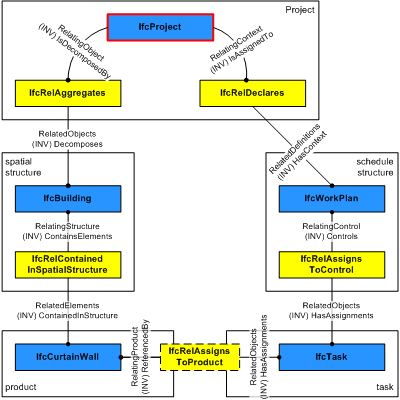
\includegraphics[width=0.6\textwidth]{principales relaciones de IfcProject}

\item IfcRelDecomposes: Se suele emplear cuando hay un árbol de jeraquia entre entidades, con una relación de parte a todo. Pudiéndose navegar desde el todo hacia sus partes, o viceversa.
\\Esta decomposición jerárquica puede ser a su vez:
\begin{itemize}
\item IfcRelNests: Se suele aplicar a entidades no físicas anidadas y con una relación de orden entre ellas. Por ejemplo a partidas de costes dentro de un presupuesto.
\item IfcRelAggregates: Se suele aplicar a objetos (entidades derivadas de IfcObjectDefinition) que forman un conjunto. En el caso de objetos físicos, la forma del conjunto se puede representar gráficamente agregando las formas de cada una de sus partes. 
\item IfcRelProjectsElement: Se suele aplicar a objetos físicos que tienen una representación proyectada sobre un plano, para relacionar el objeto con sus vistas proyectadas.
\item IfcRelVoidsElement: Se suele aplicar a objetos físicos que tienen huecos en ellos, para indicar qué otros objetos afectan/cortan al objeto.
\\ 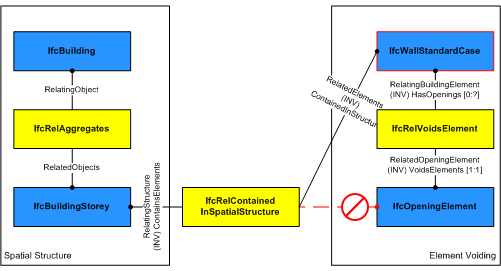
\includegraphics[width=0.8\textwidth]{relacion entre un hueco y los elementos a los que afecta}
\end{itemize}

\end{itemize}



\subsection{Asociación (IfcRelAssociates)}
\url{https://standards.buildingsmart.org/IFC/RELEASE/IFC4/ADD2_TC1/HTML/link/ifcrelassociates.htm}

Es la forma de indicar enlaces a fuentes de información internas o externas que aportan datos acerca de la entidad a la que se asocian.
\\Las fuentes más habituales suelen ser: conjuntos de propiedades, códigos de clasificación, catálogos, manuales u otros documentos, contratos, autorizaciones, certificaciones, garantias,\ldots



\subsection{Asignación (IfcRelAssigns)}
\url{https://standards.buildingsmart.org/IFC/RELEASE/IFC4/ADD2_TC1/HTML/link/ifcrelassigns.htm}

Es la forma de indicar que una entidad presta algún servicio a, es utilizada por, o tiene algún tipo de relación con otras entidades.

En un sentido amplio, se puede utilizar esta relación para navegar desde un entidad del modelo a otras con las que está relacionada. Por ejemplo, desde la tarea de ``construir fachada norte'' a la pared que hay que levantar y a las ventanas que hay que colocar en ella.

nota: Las asignaciones son bidireccionales. En el ejemplo anterior, también se puede navegar desde una de las ventanas o desde la pared a la tarea.

nota: Una asignación entre entidades no implica una dependencia entre ellas.

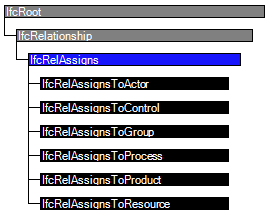
\includegraphics[scale=1]{jerarquia de IfcRelAssigns}


\subsection{Conexión (IfcRelConnects)}
\url{https://standards.buildingsmart.org/IFC/RELEASE/IFC4/ADD2_TC1/HTML/link/ifcrelconnects.htm}

Es la forma de indicar que ciertas entidades están conectadas entre sí.   Formando un ``ente'' bajo un cierto aspecto.

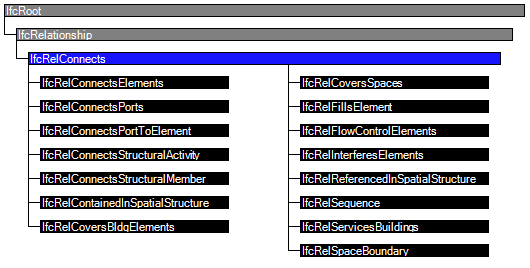
\includegraphics[width=\textwidth]{jerarquia de IfcRelConnects}

nota: Una conexión entre entidades no implica ninguna restricción respecto a cómo se comporta cada una de ellas considerada de forma individual.



\subsection{Por ejemplo, para un muro:}
Estructura de las capas que lo forman (relación con materiales)
 \\ \url{https://standards.buildingsmart.org/IFC/RELEASE/IFC4/ADD2_TC1/HTML/link/material-layer-set.htm}

Conexión con otros muros adyacentes
\\ \url{https://standards.buildingsmart.org/IFC/RELEASE/IFC4/ADD2_TC1/HTML/link/path-connectivity.htm}

Ubicación dentro del edificio o infraestructura (relación con una entidad contenedora y con unas coordenadas dentro de esta)
\\ \url{https://standards.buildingsmart.org/IFC/RELEASE/IFC4/ADD2_TC1/HTML/link/spatial-containment.htm}

Forma de su eje central (relación con una cadena de líneas y curvas 2D)
\\ \url{https://standards.buildingsmart.org/IFC/RELEASE/IFC4/ADD2_TC1/HTML/link/axis-2d-geometry.htm}

Forma de sus caras externas (relación con unas superficies 3D)
\\ \url{https://standards.buildingsmart.org/IFC/RELEASE/IFC4/ADD2_TC1/HTML/link/surface-geometry.htm}

Relaciones con otras entidades
\\ \url{https://standards.buildingsmart.org/IFC/RELEASE/IFC4/ADD2_TC1/HTML/link/product-assignment.htm}


\section{La \textbf{representación gráfica} de las entidades físicas}

Toda entidad física tiene una forma, que se suele poder mostrar representada en una imagen gráfica. Las dos maneras más habituales de representar esta forma suelen ser:
\begin{itemize}
\item Geomética: utilizando fórmulas matemáticas definidas dentro de un espacio cartesiano.
\item Topológica: utilizando puntos, aristas que unen esos puntos y caras que unen esas aristas.
\end{itemize}

\url{https://standards.buildingsmart.org/IFC/RELEASE/IFC4/ADD2_TC1/HTML/link/product-shape.htm}

\url{https://standards.buildingsmart.org/IFC/RELEASE/IFC4/ADD2_TC1/HTML/link/ifcrepresentation.htm}

\url{https://standards.buildingsmart.org/IFC/RELEASE/IFC4/ADD2_TC1/HTML/link/ifcshapemodel.htm}
\\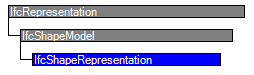
\includegraphics[width=0.5\textwidth]{jerarquia de IfcShapeRepresentation}
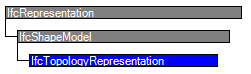
\includegraphics[width=0.5\textwidth]{jerarquia de IfcTopologyRepresentation}


\subsection{Representación de forma geométrica (IfcShapeRepresentation)}
Es una representación donde se definen formas con fórmulas matemáticas, dentro de un espacio cartesiano coordenado.

\url{https://standards.buildingsmart.org/IFC/RELEASE/IFC4/ADD2_TC1/HTML/link/ifcshaperepresentation.htm}

Esta representación utiliza diversas entidades geométricas de variadas dimensiones: puntos (entes 0D), líneas (entes 1D), superficies (entes 2D), volúmenes (entes 3D), etc.

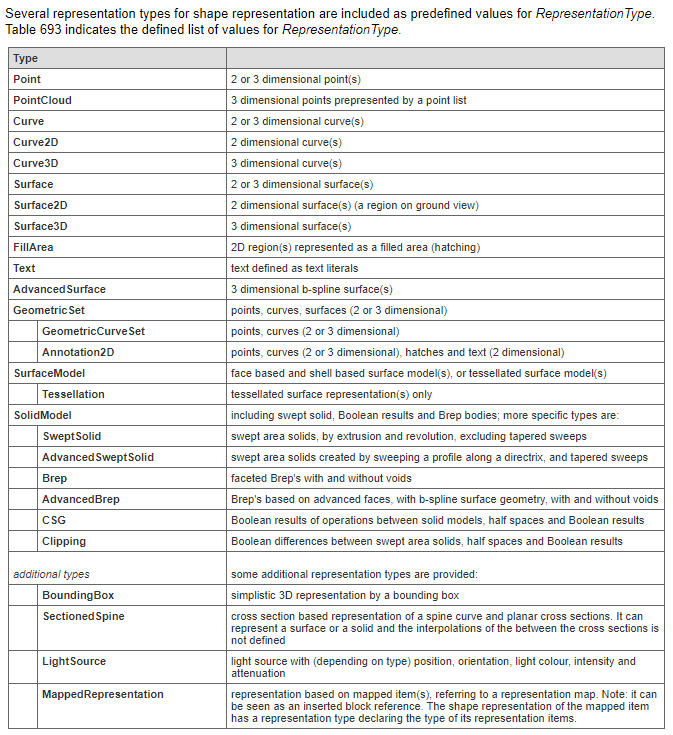
\includegraphics[width=\textwidth]{RepresentationType}

Y se puede realizar de diversas maneras: siguiendo ejes o proyecciones; mostrando una simple caja con el volumen aproximado; mostrando un perfil 2D en una vista; mostrando superficies o cuerpos sólidos con el volumen y la forma real; reservando volúmenes a respetar a su alrededor; etc.

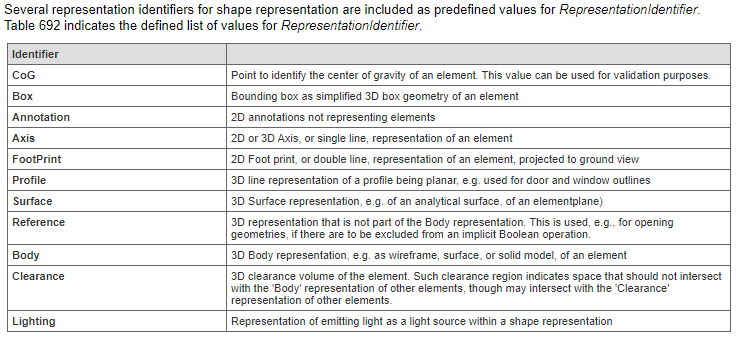
\includegraphics[width=\textwidth]{RepresentationIdentifier}


\subsection{Representación de forma topológica (IfcTopologyRepresentation)}

Es una representación donde se definen formas con vértices, aristas y caras que encierran su `cascarón' exterior.

\url{https://standards.buildingsmart.org/IFC/RELEASE/IFC4/ADD2_TC1/HTML/link/ifctopologyrepresentation.htm}


\subsection{Por ejemplo, para representar un muro de forma geométrica:}
Si sigue un eje (muro recto o muro curvo)
\\ \url{https://standards.buildingsmart.org/IFC/RELEASE/IFC4/ADD2_TC1/HTML/link/ifcboundedcurve.htm}

Si tiene formas de barrido
\\ \url{https://standards.buildingsmart.org/IFC/RELEASE/IFC4/ADD2_TC1/HTML/link/body-sweptsolid-geometry.htm}

Si tiene operaciones booleanas entre sólidos
\\ \url{https://standards.buildingsmart.org/IFC/RELEASE/IFC4/ADD2_TC1/HTML/link/body-clipping-geometry.htm}

Si tiene vaciados
\\ \url{https://standards.buildingsmart.org/IFC/RELEASE/IFC4/ADD2_TC1/HTML/link/element-voiding.htm}



\chapter{Introducción: algunos aspectos técnicos}

\section{Vistas, MVD (Model View Definition)}
\url{https://technical.buildingsmart.org/standards/ifc/mvd/}

En algunos usos, en lugar del modelo completo, suele ser conveniente intercambiar solo la parte del modelo relevante para ese uso concreto.

Las vistas MVD son una forma de utilizar solo una parte del modelo. Representan subconjuntos del esquema IFC, estandarizados para ciertos flujos de trabajo habituales.


\section{Formatos en que se puede escribir el modelo en un archivo}

\url{https://technical.buildingsmart.org/standards/ifc/ifc-formats/}

Para escribir el modelo IFC en un archivo, se puede emplear alguno de estos formatos de escritura:
\begin{itemize}

\item STEP Pysical File (con extensión .ifc): a día de hoy, es la forma habitual de escribir un archivo IFC. 
\\ \url{https://en.wikipedia.org/wiki/ISO_10303-21}
\\ \url{https://www.une.org/encuentra-tu-norma/busca-tu-norma/iso/?c=063141}

\item STEP data in XML format (con extensión .ifcXML): es una forma alternativa de escribir un archivo IFC.
\\ \url{https://en.wikipedia.org/wiki/ISO_10303-28}
\\ \url{https://www.une.org/encuentra-tu-norma/busca-tu-norma/iso/?c=040646}

\item comprimido (con extensión .ifcZIP): al ser formatos textuales, tanto SPF como XML ven reducido muchísimo su tamaño de archivo cuando se comprimen.

\item web semántica:
\\ \url{https://en.wikipedia.org/wiki/Semantic_Web}
\\ \url{https://en.wikipedia.org/wiki/Resource_Description_Framework}
\\ \url{https://technical.buildingsmart.org/standards/ifc/ifc-formats/ifcowl/}
\begin{itemize}
\item TURTLE (.ttl): 
\\ \url{https://www.w3.org/TR/turtle/}
\item RDF/XML (.rdf):
\\\url{https://www.w3.org/TR/rdf-syntax-grammar/}
\end{itemize}

\item JSON, JavaScript Object Notation (.json): a día de hoy es un formato muy popular para intercambio de datos en el mundillo web; cada vez más lenguajes de programación tienen soporte directo para él. Se está barajando como futura alternativa para los archivos IFC.
\\ \url{https://www.json.org/json-en.html}

\item HDF, Hierachical Data Format (.hdf): es un formato binario de base de datos; produce archivos muy compactos; pero no legibles por humanos (no es textual). Se está barajando como una posible futura alternativa para escribir  archivos IFC.
\\ \url{https://en.wikipedia.org/wiki/Hierarchical_Data_Format}
\\ ISO 10303-26 {\tiny \url{https://www.une.org/encuentra-tu-norma/busca-tu-norma/iso/?c=050029}}
\end{itemize}

Notas:

ISO 10303 es un estandar para intercambio de información sobre fabricación de producto. ``Standard for The Exchange of Product model data'' (STEP).

En la actualidad (2020), el formato más usado es SPF; de representación textual. Pero están ganando fuerza el formato JSON para representación textual y el HDF para representación binaria.

El formato más claro para leer es el XML.

Tanto SPF como XML suelen generar archivos bastante grandes, con muchas etiquetas repetidas. Usando compresión, se puede reducir en gran medida ese tamaño. Se suele utilizar compresión ZIP (extensión .ifcZIP).

Ejemplos para leer, de los dos formatos principales SPF(STEP) y XML, se pueden encontrar en la sección E de las especificaciones.
\\Por ejemplo, para un muro:
\\ \url{https://standards.buildingsmart.org/IFC/RELEASE/IFC4/ADD2_TC1/HTML/link/wall-standard-case.htm}
\\ejemplo en SPF: \url{https://standards.buildingsmart.org/IFC/RELEASE/IFC4/ADD2_TC1/HTML/annex/annex-e/wall-standard-case.ifc}
\\ejemplo en XML: \url{https://standards.buildingsmart.org/IFC/RELEASE/IFC4/ADD2_TC1/HTML/annex/annex-e/wall-standard-case.ifcxml} 

\section{Objetos (IfcRoot--IfcObjectDefinition--IfcObject)}
Las principales entidades (actores, controles, grupos, productos, recursos o procesos) son todas objetos.
\\ 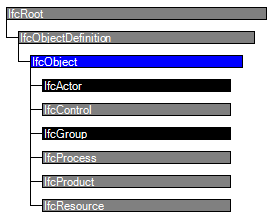
\includegraphics[width=0.5\textwidth]{jerarquia de IfcObject}
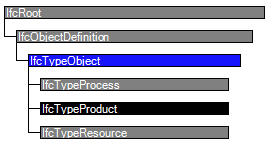
\includegraphics[width=0.5\textwidth]{jerarquia de IfcTypeObject}

Un \textit{objeto} (IfcObject) puede llevar en si mismo toda la información que lo define. O puede obtener parte de esta información desde un \textit{tipo de objeto} (IfcTypeObject) común. 

Un objeto puede constar de:
\begin{description}
\item[Definición:] su clase, su función y sus atributos intrínsecos (IfcXxxx); sus propiedades (PSet\_XxxxYyyy) y sus cuantificadores (Qto\_XxxxZzzz); otras propiedades (PSet\_---) y cuantificadores (Qto\_---) que le puedan ser de aplicación.
\item[Tipos:] parte de los atributos, propiedades o cuantificadores pueden provenir de un tipo de objeto (IfcXxxxType) común.
\item[Forma:] (si es una entidad física): su representación geométrica en 3D o en 2D.
\item[Asociaciones:] información desde fuentes externas: clasificaciones, documentos, materiales,\ldots
\item[Composición:] si el objeto está compuesto por diversas partes.
\item[Asignaciones:] si el objeto presta algún servicio a otros objetos a los que esté asignado.
\item[Conexiones:] si el objeto está conectado a otros objetos formando un ``ente'' con ellos.
\end{description}

Dentro de un modelo se insertan \textit{instancias} concretas de objetos. Cada instancia tiene sus propios valores en sus atributos, propiedades, cuantificadores, asociaciones, asignaciones, conexiones,\ldots. 

\subsection{Herencia de atributos}
Siguendo la jerarquia, un objeto tiene todos los atributos que va heredando desde sus ancestros.

Por ejemplo: IfcRoot--IfcObjectDefinition--IfcObject--IfcProduct

\url{https://standards.buildingsmart.org/IFC/RELEASE/IFC4/ADD2_TC1/HTML/link/ifcroot.htm}
\\ 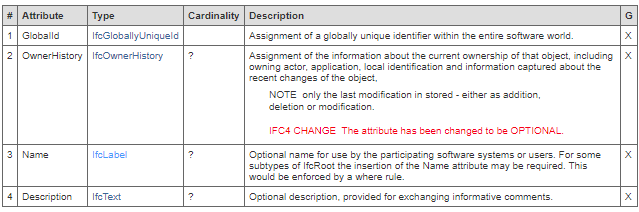
\includegraphics[width=\textwidth]{atributos de IfcRoot}
\\ \url{https://standards.buildingsmart.org/IFC/RELEASE/IFC4/ADD2_TC1/HTML/link/ifcobjectdefinition.htm}
\\ 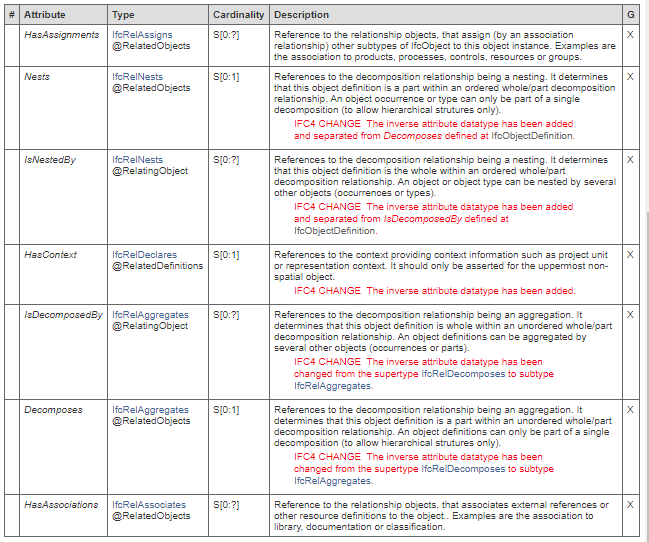
\includegraphics[width=\textwidth]{atributos de IfcObjectDefinition}

\url{https://standards.buildingsmart.org/IFC/RELEASE/IFC4/ADD2_TC1/HTML/link/ifcobject.htm}
\\ 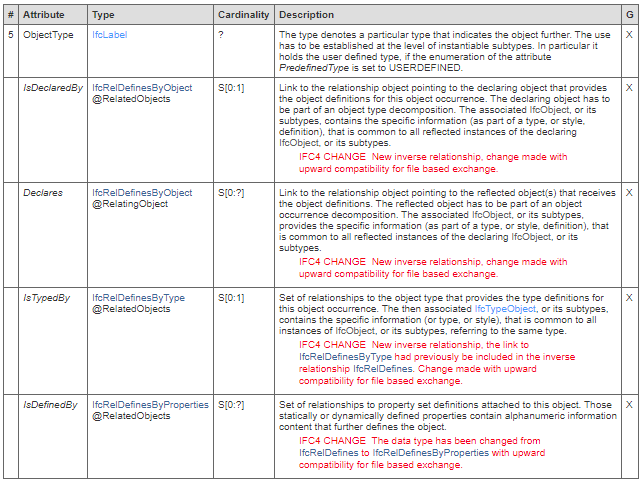
\includegraphics[width=\textwidth]{atributos de IfcObject}
\\ \url{https://standards.buildingsmart.org/IFC/RELEASE/IFC4/ADD2_TC1/HTML/link/ifcproduct.htm}
\\ 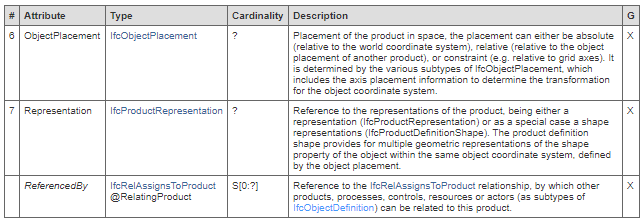
\includegraphics[width=\textwidth]{atributos de IfcProduct}

nota: IfcProduct, tiene además estos otros atributos que le vienen desde su otro ancestro, IfcTypeObject:
\\ \url{https://standards.buildingsmart.org/IFC/RELEASE/IFC4/ADD2_TC1/HTML/link/ifctypeobject.htm}
\\ 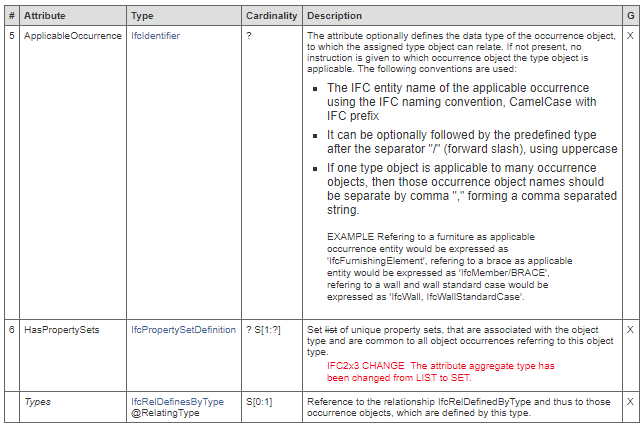
\includegraphics[width=\textwidth]{atributos de IfcTypeObject}

\vspace{0.5cm}
Más detalles sobre objetos en la sección \ref{entidades_objetos}


\subsection{Atributos inversos} \label{atributos_inversos}

Los atributos inversos suelen aparecer sobre todo en clases que representan relaciones. Toda relación se puede interpretar en uno o en otro sentido: por ejemplo, una ventana está situada sobre un hueco en un muro; pero, a su vez, el muro tiene un hueco sobre el que se sitúa una ventana.
\\ \url{https://standards.buildingsmart.org/IFC/RELEASE/IFC4/ADD2_TC1/HTML/annex/annex-e/wall-with-opening-and-window.htm}

\begin{footnotesize}
nota: En el ejemplo del enlace citado aparece una ventana (IfcWindow). Pero en el diagrama de detalle que he encontrado aparece una puerta (IfcDoor). A efectos prácticos de esta explicación, ambas son intercambiables (ambas derivan de IfcElement). 

\end{footnotesize}
Un muro (IfcWall) y un hueco (IfcOpeningElement) están relacionados con la relación IfcRelVoidsElement.
\\El hueco y una puerta (IfcDoor) están relacionados con la relación IfcRelFillsElement.

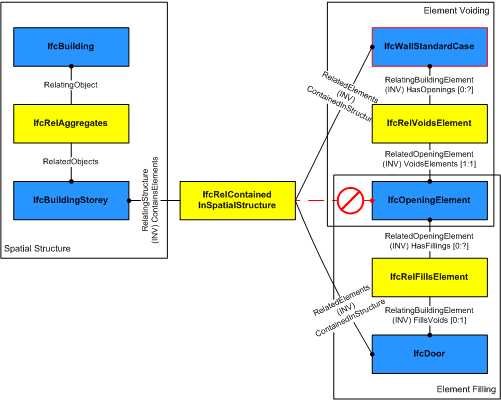
\includegraphics[width=0.8\textwidth]{ifcrelfillselements-fig1}
\begin{footnotesize}
\\ \url{https://standards.buildingsmart.org/IFC/RELEASE/IFC4/ADD2_TC1/HTML/link/ifcelement.htm}
\\ \url{https://standards.buildingsmart.org/IFC/RELEASE/IFC4/ADD2_TC1/HTML/link/ifcopeningelement.htm}
\\ \url{https://standards.buildingsmart.org/IFC/RELEASE/IFC4/ADD2_TC1/HTML/link/ifcrelvoidselement.htm}
\\ \url{https://standards.buildingsmart.org/IFC/RELEASE/IFC4/ADD2_TC1/HTML/link/ifcrelfillselement.htm}
\end{footnotesize}

La relación IfcRelVoidsElement tiene un atributo directo, RelatingBuildingElement, que admite valores de tipo IfcElement (la clase muro, IfcWall, deriva de la clase IfcElement). Pero, a su vez, el muro tiene un atributo inverso, HasOpenings, que admite valores de tipo IfcRelVoidsElement.
\vspace{0.1cm}
\\ 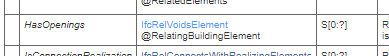
\includegraphics[scale=0.8]{atributo HasOpenings}
\vspace{0.1cm}
\\ 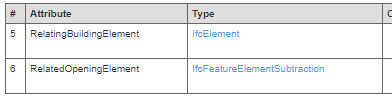
\includegraphics[scale=0.8]{atributos de IfcRelVoidsElement}
\\ 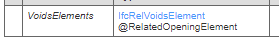
\includegraphics[scale=0.8]{atributo VoidsElements}
\\La relación IfcRelVoidsElement tiene otro atributo directo, RelatedOpeningElement, que admite valores de tipo IfcFeatureElementSubtraction (la clase hueco, IfcOpeningElement, deriva de la clase IfcFeatureElementSubstraction). Pero, a su vez, el hueco tiene un atributo inverso, VoidsElements, que admite valores de tipo IfcRelVoidsElement.

Como se ve en el gráfico, el hueco y la puerta siguen un esquema similar. Solo que con la relación IfcRelFillsElement y los atributos inversos HasFillings y FilsVoids, respectivamente.

\vspace{0.5cm}
Más detalles sobre objetos en la sección \ref{entidades_relaciones}




\newpage
\section{Conjuntos de propiedades (PSet\_ ) y de cuantificadores (Qto\_ )}

Un objeto puede tener asociados una serie de conjuntos de propiedades (PSet) con datos acerca de él y una serie de conjuntos de magnitudes (Qto) que se pueden medir sobre él.

Los conjuntos de propiedades o de magnitudes se asocian a los objetos a través del atributo `IsDefinedBy' de IfcObject, que indica relaciones `IfcRelDefinesByProperties' \url{https://standards.buildingsmart.org/IFC/RELEASE/IFC4/ADD2_TC1/HTML/link/ifcreldefinesbyproperties.htm}. 

\begin{small}
$IsDefinedBy \rightarrow RelatedObjects / RelatingPropertyDefinition \rightarrow DefinesOcurrence / HasProperties$
\end{small}
\includegraphics[width=\textwidth]{property-sets-for-objects}
\\ \url{https://standards.buildingsmart.org/IFC/RELEASE/IFC4/ADD2_TC1/HTML/link/property-sets-for-objects.htm}


\begin{small}
$IsDefinedBy \rightarrow RelatedObjects / RelatingPropertyDefinition \rightarrow DefinesOcurrence / Quantities$
\end{small}
\includegraphics[width=\textwidth]{quantity-sets}
\\ \url{https://standards.buildingsmart.org/IFC/RELEASE/IFC4/ADD2_TC1/HTML/link/quantity-sets.htm}



\section{Relaciones (IfcRelationship)}
\url{https://standards.buildingsmart.org/IFC/RELEASE/IFC4/ADD2_TC1/HTML/link/ifcrelationship.htm}

\begin{footnotesize}nota: Los enlaces a las páginas de la especificación que se dan aquí, son unos simples ejemplos. Para más detalles, seguir navegando por los enlaces en la lista que hay a la izquierda en cada página; guiarse por los números de sección para seguir la estructura lógica.\end{footnotesize}
\\ \includegraphics[width=\textwidth]{navegacion por los conceptos de la especificacion}

\subsection{Asociación (IfcRelAssociates)}
\url{https://standards.buildingsmart.org/IFC/RELEASE/IFC4/ADD2_TC1/HTML/link/ifcrelassociates.htm}

Relación en una entidad con códigos de clasificación, con documentos externos, con materiales,\ldots
\\ \url{https://standards.buildingsmart.org/IFC/RELEASE/IFC4/ADD2_TC1/HTML/link/classification.htm}
\\ \url{https://standards.buildingsmart.org/IFC/RELEASE/IFC4/ADD2_TC1/HTML/link/document-association.htm}
\\ \url{https://standards.buildingsmart.org/IFC/RELEASE/IFC4/ADD2_TC1/HTML/link/approval-association.htm}
\\ \url{https://standards.buildingsmart.org/IFC/RELEASE/IFC4/ADD2_TC1/HTML/link/constraint.htm}
\\ \url{https://standards.buildingsmart.org/IFC/RELEASE/IFC4/ADD2_TC1/HTML/link/material-association.htm}



\subsection{Composición (IfcRelDeclares -- IfcRelDecomposes)}
\url{https://standards.buildingsmart.org/IFC/RELEASE/IFC4/ADD2_TC1/HTML/link/ifcreldeclares.htm}
\\ \url{https://standards.buildingsmart.org/IFC/RELEASE/IFC4/ADD2_TC1/HTML/link/ifcreldecomposes.htm}

Relación entre un todo y sus diversas partes.
\\ \url{https://standards.buildingsmart.org/IFC/RELEASE/IFC4/ADD2_TC1/HTML/link/element-composition.htm}
\\ \url{https://standards.buildingsmart.org/IFC/RELEASE/IFC4/ADD2_TC1/HTML/link/element-decomposition.htm}
\\ \url{https://standards.buildingsmart.org/IFC/RELEASE/IFC4/ADD2_TC1/HTML/link/spatial-composition.htm}
\\ \url{https://standards.buildingsmart.org/IFC/RELEASE/IFC4/ADD2_TC1/HTML/link/spatial-decomposition.htm}
\\ \url{https://standards.buildingsmart.org/IFC/RELEASE/IFC4/ADD2_TC1/HTML/link/nesting.htm}
\\ \url{https://standards.buildingsmart.org/IFC/RELEASE/IFC4/ADD2_TC1/HTML/link/element-voiding.htm}
\\ \url{https://standards.buildingsmart.org/IFC/RELEASE/IFC4/ADD2_TC1/HTML/link/element-projecting.htm}

\subsection{Asignación (IfcRelAssigns)}
\url{https://standards.buildingsmart.org/IFC/RELEASE/IFC4/ADD2_TC1/HTML/link/ifcrelassigns.htm}

Relación entre entidades que se prestan algún servicio entre sí o entre  entidades que unas utilizan a otras para algo.
\\ \url{https://standards.buildingsmart.org/IFC/RELEASE/IFC4/ADD2_TC1/HTML/link/actor-assignment.htm}
\\ \url{https://standards.buildingsmart.org/IFC/RELEASE/IFC4/ADD2_TC1/HTML/link/control-assignment.htm}
\\ \url{https://standards.buildingsmart.org/IFC/RELEASE/IFC4/ADD2_TC1/HTML/link/group-assignment.htm}
\\ \url{https://standards.buildingsmart.org/IFC/RELEASE/IFC4/ADD2_TC1/HTML/link/product-assignment.htm}
\\ \url{https://standards.buildingsmart.org/IFC/RELEASE/IFC4/ADD2_TC1/HTML/link/process-assignment.htm}
\\ \url{https://standards.buildingsmart.org/IFC/RELEASE/IFC4/ADD2_TC1/HTML/link/resource-assignment.htm}

\subsection{Conexión (IfcRelConnects)}
\url{https://standards.buildingsmart.org/IFC/RELEASE/IFC4/ADD2_TC1/HTML/link/ifcrelconnects.htm}

Relación entre varias entidades que forman un ``ente'' entre todas ellas.
\\ \url{https://standards.buildingsmart.org/IFC/RELEASE/IFC4/ADD2_TC1/HTML/link/spatial-structure.htm}
\\ \url{https://standards.buildingsmart.org/IFC/RELEASE/IFC4/ADD2_TC1/HTML/link/space-boundaries.htm}
\\ \url{https://standards.buildingsmart.org/IFC/RELEASE/IFC4/ADD2_TC1/HTML/link/element-connectivity.htm}
\\ \url{https://standards.buildingsmart.org/IFC/RELEASE/IFC4/ADD2_TC1/HTML/link/element-filling.htm}
\\ \url{https://standards.buildingsmart.org/IFC/RELEASE/IFC4/ADD2_TC1/HTML/link/control-flow.htm}
\\ \url{https://standards.buildingsmart.org/IFC/RELEASE/IFC4/ADD2_TC1/HTML/link/structural-activity.htm}
\\ \url{https://standards.buildingsmart.org/IFC/RELEASE/IFC4/ADD2_TC1/HTML/link/structural-connectivity.htm}
\\ \url{https://standards.buildingsmart.org/IFC/RELEASE/IFC4/ADD2_TC1/HTML/link/sequential-connectivity.htm}


\vspace{0.5cm}
Más detalles sobre relaciones en la sección \ref{entidades_relaciones}



\section{Ubicación en el espacio (IfcObjectPlacement)}
\url{https://standards.buildingsmart.org/IFC/RELEASE/IFC4/ADD2_TC1/HTML/link/ifcobjectplacement.htm}

El posicionamiento indica dónde se ubica físicamente una entidad en relación con otras entidades del modelo. 

\begin{itemize}

\item IfcGridPlacement: posición relativa sobre las rejillas de referencia del proyecto.
\\ \url{https://standards.buildingsmart.org/IFC/RELEASE/IFC4/ADD2_TC1/HTML/link/ifcgridplacement.htm}
\\ \includegraphics[width=\textwidth]{atributos de IfcGridPlacement}

\item IfcLocalPlacement: posición relativa dentro del ``contenedor'' donde está colocado el objeto (por ejemplo: del emplazamiento, del edificio, de la planta,\ldots).
\\ \url{https://standards.buildingsmart.org/IFC/RELEASE/IFC4/ADD2_TC1/HTML/link/ifclocalplacement.htm}
\\ \includegraphics[width=\textwidth]{atributos de IfcLocalPlacement}
\\ \url{https://standards.buildingsmart.org/IFC/RELEASE/IFC4/ADD2_TC1/HTML/link/product-local-placement.htm}
\\ \includegraphics[width=.9\textwidth]{product-local-placement}


\end{itemize}

\subsection{Posición y Orientación (IfcPlacement)}\label{posicion_y_orientacion}

IfcPlacement es la entidad madre. Aporta atributos para indicar la posición:
\\ \url{https://standards.buildingsmart.org/IFC/RELEASE/IFC4/ADD2_TC1/HTML/link/ifcplacement.htm}
\\ \includegraphics[width=\textwidth]{atributos de IfcPlacement}
\\ \begin{footnotesize}Para más detalles, ver la sección \ref{puntos} acerca de IfcPoint.\end{footnotesize}

De ella derivan estas otras entidades que añaden atributos para indicar la orientación:
\begin{itemize}

\item IfcAxis1Placement
\\ \url{https://standards.buildingsmart.org/IFC/RELEASE/IFC4/ADD2_TC1/HTML/link/ifcaxis1placement.htm}
\\ \includegraphics[width=\textwidth]{atributos de IfcAxis1Placement}

\item IfcAxis2Placement2D
\\ \url{https://standards.buildingsmart.org/IFC/RELEASE/IFC4/ADD2_TC1/HTML/link/ifcaxis2placement2d.htm}
\\ \includegraphics[width=\textwidth]{atributos de IfcAxis2Placement2D}

\item IfcAxis2Placement3D
\\ \url{https://standards.buildingsmart.org/IFC/RELEASE/IFC4/ADD2_TC1/HTML/link/ifcaxis2placement3d.htm}
\\ \includegraphics[width=\textwidth]{atributos de IfcAxis2Placement3D}

\end{itemize}

\subsection{Entidades auxiliares:}
\begin{itemize}
\item IfcDirection
\\ \url{https://standards.buildingsmart.org/IFC/RELEASE/IFC4/ADD2_TC1/HTML/link/ifcdirection.htm}
\item IfcVector
\\ \url{https://standards.buildingsmart.org/IFC/RELEASE/IFC4/ADD2_TC1/HTML/link/ifcvector.htm}
\end{itemize}



\section{Representación grafica}
IfcPresentationResource
\\ \url{https://standards.buildingsmart.org/IFC/RELEASE/IFC4/ADD2_TC1/HTML/link/ifcrepresentationresource.htm}

\vspace{0.5cm}

IfcGeometricModelResource
\\ \url{https://standards.buildingsmart.org/IFC/RELEASE/IFC4/ADD2_TC1/HTML/link/ifcgeometricmodelresource.htm}
\\IfcGeometryResource
\\ \url{https://standards.buildingsmart.org/IFC/RELEASE/IFC4/ADD2_TC1/HTML/link/ifcgeometryresource.htm}

\vspace{0.5cm}

IfcTopologyResource
\\ \url{https://standards.buildingsmart.org/IFC/RELEASE/IFC4/ADD2_TC1/HTML/link/ifctopologyresource.htm}

\vspace{0.5cm}

IfcPresentationAppearanceResource
\\ \url{https://standards.buildingsmart.org/IFC/RELEASE/IFC4/ADD2_TC1/HTML/link/ifcpresentationappearanceresource.htm}
\\IfcPresentationDefinitionResource
\\ \url{https://standards.buildingsmart.org/IFC/RELEASE/IFC4/ADD2_TC1/HTML/link/ifcpresentationdefinitionresource.htm}
\\IfcPresentationOrganizationResource
\\ \url{https://standards.buildingsmart.org/IFC/RELEASE/IFC4/ADD2_TC1/HTML/link/ifcpresentationorganizationresource.htm}



\subsection{Representación gráfica geométrica (IfcShapeRepresentation)}
Maneras de representar un objeto físico:
\\ \url{https://standards.buildingsmart.org/IFC/RELEASE/IFC4/ADD2_TC1/HTML/link/ifcshaperepresentation.htm}
\\ \includegraphics[width=\textwidth]{RepresentationIdentifier}


\subsubsection{CoG: dibujando el centro de gravedad.}
\url{https://standards.buildingsmart.org/IFC/RELEASE/IFC4/ADD2_TC1/HTML/link/cog-geometry.htm}

\subsubsection{Box: dibujando una caja mínima que contiene el objeto.}
\url{https://standards.buildingsmart.org/IFC/RELEASE/IFC4/ADD2_TC1/HTML/link/box-geometry.htm}

\url{https://standards.buildingsmart.org/IFC/RELEASE/IFC4/ADD2_TC1/HTML/link/ifcboundingbox.htm}

\subsubsection{Annotation: dibujando cotas, etiquetas, tramas,\ldots}
\url{https://standards.buildingsmart.org/IFC/RELEASE/IFC4/ADD2_TC1/HTML/link/annotation-geometry.htm}

\subsubsection{Axis: dibujando una trayectoria.}
Por ejemplo, para muros, vigas, columnas, tuberias, conductos, cables,\ldots).
\\ \url{https://standards.buildingsmart.org/IFC/RELEASE/IFC4/ADD2_TC1/HTML/link/axis-geometry.htm}

\subsubsection{FootPrint: dibujando una superfice proyectada.}
\url{https://standards.buildingsmart.org/IFC/RELEASE/IFC4/ADD2_TC1/HTML/link/footprint-geometry.htm}

\subsubsection{Profile: dibujando una sección}
\url{https://standards.buildingsmart.org/IFC/RELEASE/IFC4/ADD2_TC1/HTML/link/profile-geometry.htm}

\subsubsection{\textbf{Surface}: dibujando una superficie.}
\url{https://standards.buildingsmart.org/IFC/RELEASE/IFC4/ADD2_TC1/HTML/link/surface-geometry.htm}

\subsubsection{Reference: ocupación de un espacio, pero sin dibujarlo.}
\url{https://standards.buildingsmart.org/IFC/RELEASE/IFC4/ADD2_TC1/HTML/link/reference-geometry.htm}

\subsubsection{\textbf{Body}: dibujando un cuerpo.}
\url{https://standards.buildingsmart.org/IFC/RELEASE/IFC4/ADD2_TC1/HTML/link/body-geometry.htm}

\begin{itemize}
\item Con un volumen extruido.
\\ \url{https://standards.buildingsmart.org/IFC/RELEASE/IFC4/ADD2_TC1/HTML/link/ifcsweptsurface.htm}

\item Con un volumen de revolución.
\\ \url{https://standards.buildingsmart.org/IFC/RELEASE/IFC4/ADD2_TC1/HTML/link/ifcsurfaceofrevolution.htm}

\item Utilizando volúmenes primitivos (paralelepípedos, cilindros, conos, pirámides,\ldots), combinados mediante operaciones booleanas de adicción/substracción entre ellos.

\item Con un volumen ``cascarón'', definido por sus superficies exteriores

\item \ldots
\end{itemize}

\subsubsection{Clearance: reservando un espacio libre alrededor de\ldots}
\url{https://standards.buildingsmart.org/IFC/RELEASE/IFC4/ADD2_TC1/HTML/link/clearance-geometry.htm}

\subsubsection{Lighting: espacio iluminado por lámparas y luminarias.}
\url{https://standards.buildingsmart.org/IFC/RELEASE/IFC4/ADD2_TC1/HTML/link/lighting-geometry.htm}

\subsubsection{Survey Points: para definir líneas de contorno del terreno.}
\url{https://standards.buildingsmart.org/IFC/RELEASE/IFC4/ADD2_TC1/HTML/link/survey-points-geometry.htm}

\subsubsection{Mapped: para insertar instancias en distintas posiciones y orientaciones}
\url{https://standards.buildingsmart.org/IFC/RELEASE/IFC4/ADD2_TC1/HTML/link/mapped-geometry.htm}

\vspace{0.5cm}
Más detalles sobre representación gráfica geométrica en el capítulo \ref{entidades_geometria}



\subsection{Representación gráfica topológica (IfcTopologyRepresentation)}
\url{https://standards.buildingsmart.org/IFC/RELEASE/IFC4/ADD2_TC1/HTML/link/ifctopologyrepresentation.htm}


\subsubsection{vértices}
\url{https://standards.buildingsmart.org/IFC/RELEASE/IFC4/ADD2_TC1/HTML/link/ifcvertex.htm}

\subsubsection{aristas}
\url{https://standards.buildingsmart.org/IFC/RELEASE/IFC4/ADD2_TC1/HTML/link/ifcedge.htm}

\subsubsection{caras}
\url{https://standards.buildingsmart.org/IFC/RELEASE/IFC4/ADD2_TC1/HTML/link/ifcface.htm} 

\subsubsection{conjuntos}
\url{https://standards.buildingsmart.org/IFC/RELEASE/IFC4/ADD2_TC1/HTML/link/ifcshell.htm}

\vspace{0.5cm}
Más detalles sobre representación gráfica topológica en el capítulo \ref{entidades_topologia}



\subsection{Traslación, rotación, escalado y simetria \\ (IfcCartesianTransformationOperator)}
\url{https://standards.buildingsmart.org/IFC/RELEASE/IFC4/ADD2_TC1/HTML/link/ifccartesiantransformationoperator.htm}



\subsection{Estilos de presentación (IfcPresentationStyle)}
\url{https://standards.buildingsmart.org/IFC/RELEASE/IFC4/ADD2_TC1/HTML/link/ifcpresentationstyle.htm}

IfcTextStyle
\\ \url{https://standards.buildingsmart.org/IFC/RELEASE/IFC4/ADD2_TC1/HTML/link/ifctextstyle.htm}

IfcFillAreaStyle
\\ \url{https://standards.buildingsmart.org/IFC/RELEASE/IFC4/ADD2_TC1/HTML/link/ifcfillareastyle.htm}

IfcCurveStyle
\\ \url{https://standards.buildingsmart.org/IFC/RELEASE/IFC4/ADD2_TC1/HTML/link/ifccurvestyle.htm}

IfcSurfaceStyle
\\ \url{https://standards.buildingsmart.org/IFC/RELEASE/IFC4/ADD2_TC1/HTML/link/ifcsurfacestyle.htm}

IfcPresentationLayerAssignmentWithStyle
\\ \url{https://standards.buildingsmart.org/IFC/RELEASE/IFC4/ADD2_TC1/HTML/link/ifcpresentationlayerwithstyle.htm}

\subsection{Texturas (IfcSurfaceTexture)}
\url{https://standards.buildingsmart.org/IFC/RELEASE/IFC4/ADD2_TC1/HTML/link/ifcsurfacetexture.htm}

IfcBlobTexture
\\ \url{https://standards.buildingsmart.org/IFC/RELEASE/IFC4/ADD2_TC1/HTML/link/ifcblobtexture.htm}

IfcImageTexture
\\ \url{https://standards.buildingsmart.org/IFC/RELEASE/IFC4/ADD2_TC1/HTML/link/ifcimagetexture.htm}

IfcPixelTexture
\\ \url{https://standards.buildingsmart.org/IFC/RELEASE/IFC4/ADD2_TC1/HTML/link/ifcpixeltexture.htm}


\subsection{Iluminación (IfcLightSource)}
\url{https://standards.buildingsmart.org/IFC/RELEASE/IFC4/ADD2_TC1/HTML/link/ifclightsource.htm}

IfcLightSourceAmbient
\\ \url{https://standards.buildingsmart.org/IFC/RELEASE/IFC4/ADD2_TC1/HTML/link/ifclightsourceambient.htm}

IfcLightSourceDirectional
\\ \url{https://standards.buildingsmart.org/IFC/RELEASE/IFC4/ADD2_TC1/HTML/link/ifclightsourcedirectional.htm}

IfcLightSourceGoniometric
\\ \url{https://standards.buildingsmart.org/IFC/RELEASE/IFC4/ADD2_TC1/HTML/link/ifclightsourcegoniometric.htm}

IfcLightSourcePositional
\\ \url{https://standards.buildingsmart.org/IFC/RELEASE/IFC4/ADD2_TC1/HTML/link/ifclightsourcepositional.htm}



\chapter{Entidades base}

\section{IfcRoot, la madre principal de la que derivan gran parte de todas las demás entidades}
\url{https://standards.buildingsmart.org/IFC/RELEASE/IFC4/ADD2_TC1/HTML/link/ifcroot.htm}

IfcRoot es la madre que aporta, a todas las entidades que de ella derivan, los atributos:

\begin{longtable}{|p{2.5cm}p{11cm}|}
\hline

\textbf{GlobalId} & Un código único que identifica cada entidad concreta que aparece en un modelo. Es un número aleatório, autogenerado, de 128 bits ($2^{128} \simeq 10^{38}$ posibles códigos). No se repite para ninguna entidad en ningún modelo. Es decir, es realmente un identificador único a nivel global: no puede haber \begin{footnotesize}(*)\end{footnotesize} dos modelos con sendas entidades con el mismo id en ningún projecto, en ninguna parte del mundo.
\newline \url{https://standards.buildingsmart.org/IFC/RELEASE/IFC4/ADD2_TC1/HTML/link/ifcgloballyuniqueid.htm}
\newline \begin{footnotesize}(*) Bueno, realmente poder\ldots, podria suceder que se generara el mismo Id para dos entidades; pero la probabilidad de que eso suceda es menor que la de que un asteroide impacte la Tierra y nos extinga a todos los humanos.\end{footnotesize}
\\[0.1cm] \hline

OwnerHistory & Información acerca de quién, cuándo y con qué aplicación ha creado la entidad. E información acerca de las modificaciones que ha tenido la entidad (control de cambios).
\newline \url{https://standards.buildingsmart.org/IFC/RELEASE/IFC4/ADD2_TC1/HTML/link/ifcownerhistory.htm}
\\[0.1cm] \hline

\textbf{Name} & Un nombre (más o menos corto), legible para humanos.
\newline \url{https://standards.buildingsmart.org/IFC/RELEASE/IFC4/ADD2_TC1/HTML/link/ifclabel.htm}
\\[0.1cm] \hline

\textbf{Description} & Una descripción (más o menos larga), legible para humanos.
\newline \url{https://standards.buildingsmart.org/IFC/RELEASE/IFC4/ADD2_TC1/HTML/link/ifctext.htm}
\\[0.1cm] \hline

\end{longtable}




\section{IfcRelationship, la madre de las relaciones entre entidades} \label{entidades_relaciones}
\url{https://standards.buildingsmart.org/IFC/RELEASE/IFC4/ADD2_TC1/HTML/link/ifcrelationship.htm}
\\ \includegraphics[width=\textwidth]{jerarquia de IfcRelationship}


\subsection{IfcRelAssigns: enlaces genéricos entre objetos relacionados}
\url{https://standards.buildingsmart.org/IFC/RELEASE/IFC4/ADD2_TC1/HTML/link/ifcrelassigns.htm}

Expresa un enlace entre un objeto y otros. Bien porque le suministran algún servicio o bien porque están relacionados de alguna manera con él.

Los objetos relacionados se indican en el atributo (RelatedObjects) de la asignación.

Las asignaciones son bidireccionales. Permiten navegar desde el objeto a sus asignados o, viceversa, desde los asignados al objeto.

Una asignación entre objetos no implica una dependencia entre ellos.

Si la asignación es con una modalidad de objeto concreto, se puede emplear una de estas entidades especializadas para expresarla:
\begin{itemize}

\item \textbf{IfcRelAssignsToProduct}: Establece con qué producto tiene relación (RelatingProduct).

\item \textbf{IfcRelAssignsToResource}: Establece con qué recurso tiene relación (RelatingResource).

\item \textbf{IfcRelAssignsToProcess}: Establece con qué proceso  (RelatingProcess) y la cantidad utilizada en el proceso (QuantityInProcess).

\item \textbf{IfcRelAssignsToActor}: Establece con qué actor (RelatingActor) y qué rol desempeña este en la relación (ActingRole).

\item \textbf{IfcRelAssignsToControl}: Establece con qué control tiene relación (RelatingControl).

\item \textbf{IfcRelAssignsToGroup}: Establece con qué grupo tiene relación (RelatingGroup).

\end{itemize}


\subsection{IfcRelAssociates: enlaces con fuentes de información}
\url{https://standards.buildingsmart.org/IFC/RELEASE/IFC4/ADD2_TC1/HTML/link/ifcrelassociates.htm}

Expresa un enlace entre un objeto y fuentes de información que pueden aportar datos acerca de él.

Las entidades o propiedades asociadas como fuente de información se indican en el atributo RelatedObjects de la asociación.

Si la asociación es con una fuente de información concreta, se puede emplear una de estas entidades especializadas para expresarla:
\begin{itemize}

\item \textbf{IfcRelAssociatesApproval}: autorizaciones formales.
\\(IfcApproval) \url{https://standards.buildingsmart.org/IFC/RELEASE/IFC4/ADD2_TC1/HTML/link/ifcapproval.htm}

\item \textbf{IfcRelAssociatesClassification}: sistemas de clasificación para partidas en presupuestos.
\\(IfcClassification) \url{https://standards.buildingsmart.org/IFC/RELEASE/IFC4/ADD2_TC1/HTML/link/ifcclassification.htm}

\item \textbf{IfcRelAssociatesConstraint}: límites.
\\(IfcConstraint) \url{https://standards.buildingsmart.org/IFC/RELEASE/IFC4/ADD2_TC1/HTML/link/ifcconstraint.htm}

\item \textbf{IfcRelAssociatesDocument}: bibliografia, documentos sueltos.
\\(IfcDocumentInformation) \url{https://standards.buildingsmart.org/IFC/RELEASE/IFC4/ADD2_TC1/HTML/link/ifcdocumentinformation.htm}

\item \textbf{IfcRelAssociatesLibrary}: repositorios organizados de documentación, conjuntos de documentos.
\\(IfcLibraryInformation) \url{https://standards.buildingsmart.org/IFC/RELEASE/IFC4/ADD2_TC1/HTML/link/ifclibraryinformation.htm}

\item \textbf{IfcRelAssociatesMaterial}: substancias materiales de las que está hecho el objeto.
\\ \url{https://standards.buildingsmart.org/IFC/RELEASE/IFC4/ADD2_TC1/HTML/link/ifcmaterialselect.htm}

\end{itemize}



\subsection{IfcRelConnects: conexiones entre objetos unidos o relacionados entre sí de algún modo}
\url{https://standards.buildingsmart.org/IFC/RELEASE/IFC4/ADD2_TC1/HTML/link/ifcrelconnects.htm}

Expresa conexiones entre objetos que se unen entre sí para formar entidades más grandes, de acuerdo a un determinado fin.

Una conexión entre objetos no implica una restricción sobre ninguno de ellos considerados por separado.

La conexión puede ser una de estas:
\begin{itemize}

\item \textbf{IfcRelContainedInSpatialStructure}: Un grupo de objetos (RelatedElements) pueden estar incluidos en un ``contenedor'' (RelatingStructure) tal como un piso de un edificio.
\\ \url{https://standards.buildingsmart.org/IFC/RELEASE/IFC4/ADD2_TC1/HTML/link/ifcrelcontainedinspatialstructure.htm}

\item \textbf{IfcRelReferencedInSpatialStructure}: Pero aunque estén incluidos en un ``contenedor'', también pueden pertenecer a otros ``contenedores''. Por ejemplo, un muro cortina comienza en un piso, pero puede extenderse por varios otros pisos del edificio.
\\ \url{https://standards.buildingsmart.org/IFC/RELEASE/IFC4/ADD2_TC1/HTML/link/ifcrelreferencedinspatialstructure.htm}

\item \textbf{IfcRelCoversBldgElements}: Un objeto (RelatingBuildingElement) puede estar recubierto por otros (RelatedCoverings) que le sirven de acabado superficial.
\\ \url{https://standards.buildingsmart.org/IFC/RELEASE/IFC4/ADD2_TC1/HTML/link/ifccovering.htm}

\item \textbf{IfcRelFillsElement}: Un hueco (RelatingOpeningElement) cortado en un objeto puede estar ocupado por otro objeto (RelatedBuildingElement).

\item \textbf{IfcRelSpaceBoundary}: Una entidad (RelatedBuildingElement) sirve como delimitador para una zona (RelatingSpace) en alguna parte del borde que delimita la zona.
\\ \url{https://standards.buildingsmart.org/IFC/RELEASE/IFC4/ADD2_TC1/HTML/link/ifcrelspaceboundary.htm}

\item \textbf{IfcRelConnectsElements}: Expresa una conexión genérica entre objetos IfcElement. Las entidades conectadas se indican en los atributos (RelatingElement) y (RelatedElement), respectivamente. En el atributo (ConnectionGeometry) se puede indicar una representación gráfica para visibilizar la conexión en el modelo.

\item \textbf{IfcRelConnectsPorts}: Expresa una conexión genérica entre puertos (puntos de conexión que tienen algunos objetos).

\item \textbf{IfcRelConnectsPortToElement}:

\item \textbf{IfcRelConnectsStructuralActivity}: Expresa la acción de una fuerza sobre un determinado elemento estructural.

\item \textbf{IfcRelConnectsStructuralMember}: Expresa la acción de un apoyo o restricción sobre un determinado elemento estructural.
\\ \url{https://standards.buildingsmart.org/IFC/RELEASE/IFC4/ADD2_TC1/HTML/link/ifcrelconnectsstructuralmember.htm}

\item \textbf{IfcRelFlowControlElements}: Un elemento de control de flujo (RelatingFlowElement) en una instalación de fontaneria, electricidad, aireación,\ldots puede estar controlado por otros elementos (RelatedControlElements).

\item \textbf{IfcRelSequence}: Un proceso (RelatedProcess) sucede a otro (RelatingProcess) en una secuencia. Con una duración (TimeLag) aplicada de una determinada forma \url{https://standards.buildingsmart.org/IFC/RELEASE/IFC4/ADD2_TC1/HTML/link/ifcsequenceenum.htm}

\item \textbf{IfcRelServicesBuildings}: Una instalación (RelatingSystem) da servicio a un emplazamiento, a un edificio, a un piso del edificio, a una zona del edificio,\ldots (RelatedBuildings)

\item \textbf{IfcRelInterferesElements}: Se usa para marcar interferencias entre elementos que se solapan sin que debieran solaparse. [Clash Detection]
\\ \url{https://standards.buildingsmart.org/IFC/RELEASE/IFC4/ADD2_TC1/HTML/link/ifcrelinterfereselements.htm}

\end{itemize}


\subsection{IfcRelDeclares: inclusión de objetos o propiedades dentro del modelo}
\url{https://standards.buildingsmart.org/IFC/RELEASE/IFC4/ADD2_TC1/HTML/link/ifcreldeclares.htm}

Expresa la inclusión de objetos (derivados de IfcObject) o propiedades (derivados de IfcPropertyDefinition) dentro del modelo (IfcProject o IfcProjectLibrary)



\subsection{IfcRelDecomposes: desglose o despiece de objetos compuestos}
\url{https://standards.buildingsmart.org/IFC/RELEASE/IFC4/ADD2_TC1/HTML/link/ifcreldecomposes.htm}

Expresa el hecho de que un objeto esté compuesto por partes contenidas dentro de él.

Esta relación del todo con sus partes puede ser una de estas:
\begin{itemize}

\item \textbf{IfcRelAggregates}: Implica una relación de inclusión, unas entidades son partes integrantes dentro de otras.

\item \textbf{IfcRelNests}: Implica una relación de orden, unas entidades van a continuación de otras. Todas las entidades participantes en la relación han de ser del mismo tipo.

\item \textbf{IfcRelProjectsElement}: Es un modificador de la representación gráfica del objeto,  projectandolo sobre otro.

\item \textbf{IfcVoidsElement}: Relaciona un objeto con otros objetos que lo cortan para crear huecos en él.

\end{itemize}


\subsection{IfcRelDefines: relación de un objeto con tipos o con conjuntos de propiedades}
\url{https://standards.buildingsmart.org/IFC/RELEASE/IFC4/ADD2_TC1/HTML/link/ifcreldefines.htm}

Expresa una relación:
\begin{itemize}
\item De un tipo de objeto a una ocurrencia del mismo.
\item De un conjunto de propiedades a una instancia de un objeto.
\item De una plantilla a un conjunto de propiedades.
\end{itemize}

Según qué se relaciona con qué, la relación puede ser una de estas:
\begin{itemize}

\item \textbf{IfcRelDefinesByObject}: relaciona instancias de objetos (RelatedObjects) con  la definición de un objeto determinado (RelatingObject)

\item \textbf{IfcRelDefinesByType}: relaciona instancias de objetos (RelatedObjects) con la definición de un tipo de objeto determinado (RelatingType).

\item \textbf{IfcRelDefinesByProperties}: relaciona instancias de objetos (RelatedObjects) con un determinado conjunto de propiedades o un determinado conjunto de cuantificadores (RelatingPropertyDefinition).

\item \textbf{IfcRelDefinesByTemplate}: relaciona conjuntos de propiedades (RelatedPropertySets) con una determinada definición de un conjunto de propiedades (RelatingTemplate)


\end{itemize}



\section{IfcObjectDefinition-IfcObject-IfcTypeObject, las madres de los objetos} \label{entidades_objetos}

\begin{large}\textbf{IfcObjectDefinition}\end{large}
\\ \url{https://standards.buildingsmart.org/IFC/RELEASE/IFC4/ADD2_TC1/HTML/link/ifcobjectdefinition.htm}

IfcObjectDefinition es la madre que aporta, a todos los objetos que de ella derivan, los atributos:

\begin{longtable}{|p{2.5cm} p{11cm}|}
\hline

\textbf{HasAsssignments}: & (IfcRelAssings) Es un atributo inverso \footnote{}, permite saber qué otros objetos se relacionan con este objeto.
\\[0.1cm] \hline

\textbf{Nests}: & (IfcRelNests) Es un atributo inverso \footnote{}, permite saber qué objeto precede a este dentro de una secuencia ordenada.
\\[0.1cm] \hline

IsNestedBy: & (IfcRelNests) Es un atributo inverso \footnote{}, permite saber qué otros objetos siguen a este dentro de una secuencia ordenada. Recoge todas las partes que integran este objeto.
\\[0.1cm] \hline

\textbf{HasContext}: & (IfcRelDeclares) Es un atributo inverso \footnote{}, permite saber la entidad que aporta información de contexto este objeto.
\\[0.1cm] \hline

\textbf{Decomposes}: & (IfcRelAggregates) Es un atributo inverso \footnote{}, permite saber de qué otro objeto este forma parte. Indica que este objeto es parte de otro.
\\[0.1cm] \hline

IsDecomposedBy: & (IfcRelAggregates) Es un atributo inverso \footnote{}, permite saber qué otros objetos forman parte de este. Recoge todas las partes que integran este objeto.
\\[0.1cm] \hline

\textbf{HasAssociations}: & (IfcRelAssociates) Es un atributo inverso \footnote{}, permite saber qué otras entidades están relacionadas con este objeto para aportarle datos. Por ejemplo: conjuntos de propiedades (PSets), hojas de especificaciones, catálogos, manuales de uso,\ldots
\\[0.1cm] \hline

\end{longtable}
\footnote{Ver \ref{atributos_inversos} para una explicación sobre las relaciones y los atributos inversos}



\vspace{0.5cm}

\begin{large}\textbf{IfcObject}\end{large}
\\ \url{https://standards.buildingsmart.org/IFC/RELEASE/IFC4/ADD2_TC1/HTML/link/ifcobject.htm}

IfcObject es una especialización de IfcObjectDefinition y aporta más atributos a los objetos que de ella derivan:

\begin{longtable}{|p{2.5cm} p{11cm}|}
\hline

ObjectType: & (IfcLabel) Una etiqueta (texto) que indica el tipo de objeto que es, si es que este es un objeto de un tipo determinado. 
\\[0.1cm] \hline

IsDeclaredBy: & (IfcRelDefinesByObject) Es un atributo inverso \footnote{}, permite saber qué otro objeto define a este.
\\[0.1cm] \hline

Declares: & (IfcRelDefinesByObject)  Es un atributo inverso \footnote{}, permite saber qué otros objetos son definidos por este.
\\[0.1cm] \hline

IsTypedBy: & (IfcRelDefinesByType) Es un atributo inverso \footnote{}, permite saber de qué tipo es el objeto.
\\[0.1cm] \hline

IsDefinedBy: & (IfcRelDefinesByProperties) Es un atributo inverso \footnote{}, que permite saber qué conjuntos de propiedades están asociados a este objeto.
\\[0.1cm] \hline

\end{longtable}


\vspace{0.5cm}

\begin{large}\textbf{IfcTypeObject}\end{large}
\\ \url{https://standards.buildingsmart.org/IFC/RELEASE/IFC4/ADD2_TC1/HTML/link/ifctypeobject.htm}

IfcTypeObject es una especialización de IfcObjectDefinition y aporta más atributos a los objetos que de ella derivan:

\begin{longtable}{|p{3cm} p{10cm}|}
\hline

ApplicableOccurrence & (IfcIdentifier) A qué clases de objetos puede aplicarse este tipo.
\\[0.1cm] \hline

HasPropertySets & (IfcPropertySetDefinition) Lista de conjuntos de propiedades asociados a este tipo.
\\[0.1cm] \hline

Types & (IfcRelDefinesByType) Es un atributo inverso \footnote{•}, permite saber qué otros objetos son definidos por este tipo.
\\[0.1cm] \hline

\end{longtable}
\footnote{Ver \ref{atributos_inversos} para una explicación sobre las relaciones y los atributos inversos}


\vspace{0.5cm}



\subsection{Productos (IfcProduct)}
\url{https://standards.buildingsmart.org/IFC/RELEASE/IFC4/ADD2_TC1/HTML/link/ifcproduct.htm}

IfcProduct es una especialización de IfcObject que representa algo directamente relacionado con un objeto final en la construcción física. Aporta estos atributos adicionales:

\begin{longtable}{|p{2.5cm} p{11cm}|}
\hline

\textbf{ObjectPlacement} & (IfcObjectPlacement) El lugar donde el producto va colocado dentro del modelo. Esta ubicación puede ser:
\begin{itemize}
\item Absoluta: tomando como referencia el sistema de coordenadas global del ``mundo'', el sistema de coordenadas general del modelo. 
\item Relativa: tomando como referencia la ubicación de otro objeto.
\item Restringida: tomando como referencia un eje de una rejilla.
\end{itemize}
\\[0.1cm] \hline

\textbf{Representation} & (IfcProductRepresentation) La representación gráfica del producto, la forma de dibujarlo.
\\[0.1cm] \hline

ReferencedBy & (IfcRelAssignsToProduct) Es un atributo inverso, permite saber qué otros objetos han sido asignados a este producto.
\\[0.1cm] \hline

\end{longtable}

\vspace{0.3cm}
Algunas modalidades concretas de producto tienen sus propias entidades especializadas para designarlas:

\begin{itemize}

\item \textbf{IfcElement}: La mayoria de los objetos físicos que se colocan dentro de la construcción derivan de esta entidad.
\\ \url{https://standards.buildingsmart.org/IFC/RELEASE/IFC4/ADD2_TC1/HTML/link/ifcelement.htm}

El elemento aporta al producto estos atributos adicionales:
\\ \begin{longtable}{|p{3.5cm} p{10cm}|}
\hline

Tag & Un identificador para el elemento. Por ejemplo, un número de serie.
\\[0.1cm] \hline

ContainedInStructure & (IfcRelContainedInSpatialStructure) Es un atributo inverso \footnote{•}, permite saber la estructura espacial (``contenedor'') principal dentro de la cual está ubicado este elemento.
\\[0.1cm] \hline

ReferencedInStructures & (IfcRelReferencedInSpatialStructure) Es un atributo inverso \footnote{•}, permite saber dentro de qué otras estructuras espaciales está también este elemento.
\\[0.1cm] \hline

ProvidesBoundaries & (IfcRelSpaceBoundary) Es un atributo inverso \footnote{•}, permite saber qué espacios o zonas limita este elemento.
\\[0.1cm] \hline

ConnectedFrom & (IfcRelConnectsElements) Es un atributo inverso \footnote{•}, permite saber los elementos que están conectados con este.
\\[0.1cm] \hline

ConnectedTo & (IfcRelConnectsElements) Es un atributo inverso \footnote{•}, permite saber a qué otros elementos está conectado este.
\\[0.1cm] \hline

IsConnectionRealization & (IfcRelConnectsWithRealizingElements) Es un atributo inverso \footnote{•}, permite saber  todos los objetos que ?
\\[0.1cm] \hline

IsInterferedByElements & (IfcRelInterferesElements) Es un atributo inverso \footnote{•}, permite saber todos los objetos que tienen alguna interfencia con este.
\\[0.1cm] \hline

InterferesElements & (IfcRelInterferesElements) Es un atributo inverso \footnote{•}, permite saber con qué otros elementos este interfiere de alguna manera. 
\\[0.1cm] \hline

FillsVoids & (IfcRelFillsElement) Es un atributo inverso \footnote{•}, permite saber en qué otro elemento este rellena un hueco.
\\[0.1cm] \hline

HasOpenings & (IfcRelVoidsElement) Es un atributo inverso \footnote{•}, permite saber qué huecos cortan este elemento. 
\\[0.1cm] \hline

HasCoverings & (IfcRelCoversBldgElements) Es un atributo inverso \footnote{•}, permite saber  qué otros elementos cubren a este y le aportan su acabado. \newline \url{https://standards.buildingsmart.org/IFC/RELEASE/IFC4/ADD2_TC1/HTML/link/ifccovering.htm}
\\[0.1cm] \hline

HasProjections & (IfcRelProjectsElement) Es un atributo inverso \footnote{•}, permite saber qué otros objetos se proyectan (unión booleana) sobre este.
\\[0.1cm] \hline

\end{longtable}
\footnote{Ver \ref{atributos_inversos} para una explicación sobre las relaciones y los atributos inversos}


\vspace{0.3cm}
IfcElement tiene a su vez una serie de modalidades de elemento que lo especializan aún más:
\begin{itemize}
\item \textbf{IfcBuildingElement}: cimentaciones, muros, losas, columnas, vigas, ventanas,\ldots
\\ \url{https://standards.buildingsmart.org/IFC/RELEASE/IFC4/ADD2_TC1/HTML/link/ifcbuildingelement.htm}
\item \textbf{IfcCivilElement}: en la versión 4.3 de las especificaciones IFC se están definiendo entidades específicas para este tipo de objetos, ver más adelante en el capítulo \ref{entidades_infraestructuras}.
\item \textbf{IfcDistributionElement}: elementos relacionados con los sistemas electricos, HVAC y fontaneria.
\\Elementos de monitorización y control: actuadores, reguladores, sensores, alarmas,\ldots 
\\ \url{https://standards.buildingsmart.org/IFC/RELEASE/IFC4/ADD2_TC1/HTML/link/ifcdistributioncontrolelement.htm}
\\Elementos que componen las propias instalaciones en sí: tuberias, cableados, conductos, depósitos, protecciones,\ldots Y  elementos terminales que están conectados a ellas: enchufes, salidas de aire, radiadores, lavabos, lámparas, equipos musicales,\ldots
\\ \url{https://standards.buildingsmart.org/IFC/RELEASE/IFC4/ADD2_TC1/HTML/link/ifcdistributionflowelement.htm}
\item \textbf{IfcElementAssembly}: agregaciones complejas de objetos.
\item \textbf{IfcElementComponent}: objetos auxiliares tales como tornillos, soportes, tendones de pretensado, ferralla,\ldots
\\ \url{https://standards.buildingsmart.org/IFC/RELEASE/IFC4/ADD2_TC1/HTML/link/ifcelementcomponent.htm}
\item \textbf{IfcFeatureElement}: accesorios que modifican la forma de otro objeto; por ejemplo: embellecedores, huecos,\ldots
\item \textbf{IfcFurnisingElement}: mobiliario.
\item \textbf{IfcGeographicElement}: terreno, árboles, estanques, fuentes, bancos, marquesinas,\ldots 
\item \textbf{IfcTransportElement}: escaleras mecánicas,ascensores,\ldots
\item \textbf{IfcVirtualElement}: se utilizan para delimitar espacios imaginarios; por ejemplo: pasillos mínimos a dejar libres para vias de evacuación, separaciones conceptuales según usos dentro de un espacio diáfano,\ldots
\end{itemize}

\item \textbf{IfcSpatialElement}, \textbf{IfcSpatialStructureElement}, \textbf{IfcSpatialZone}:
\\Los ``contenedores de objetos'' o los ``espacios funcionales'' derivan de estas entidades.
\\ \url{https://standards.buildingsmart.org/IFC/RELEASE/IFC4/ADD2_TC1/HTML/link/ifcspatialelement.htm}
\\ \url{https://standards.buildingsmart.org/IFC/RELEASE/IFC4/ADD2_TC1/HTML/link/ifcspatialstructureelement.htm}

El elemento espacial aporta al producto estos atributos adicionales:
\\ \begin{longtable}{|p{2.5cm} p{11cm}|}
\hline

LongName & Una descripción informal.
\\[0.1cm] \hline

ContainsElements & (IfcRelContainedInSpatialStructure) Es un atributo inverso \footnote{•}, permite saber los objetos que están dentro de esta estructura.
\\[0.1cm] \hline

ReferencesElements & (IfcRelReferencedInSpatialStructure) Es un atributo inverso \footnote{•}, permite saber los objetos que tienen relación con esta estructura.
\\[0.1cm] \hline

ServicedBySystems & (IfcRelServicesBuildins) Es un atributo inverso \footnote{•}, permite saber las instalaciones que dan servicio a esta estructura.
\\[0.1cm] \hline

\end{longtable}
\footnote{Ver \ref{atributos_inversos} para una explicación sobre las relaciones y los atributos inversos}


\item \textbf{IfcPort}: los puntos de anclaje para conectar (IfcRelNests) unos objetos con otros derivan de esta entidad.

El puerto aporta al producto estos atributos adicionales:
\\ \begin{longtable}{|p{2.5cm} p{11cm}|}
\hline
ContainedIn & 
\\[0.1cm] \hline
ConnectedFrom & 
\\[0.1cm] \hline
ConnectedTo &
\\[0.1cm] \hline
\end{longtable}

\item \textbf{IfcStructuralItem}, \textbf{IfcStructuralConnection}, \textbf{IfcStructuralMember}: Los objetos estructurales derivan de esta entidad.
\\ \url{https://standards.buildingsmart.org/IFC/RELEASE/IFC4/ADD2_TC1/HTML/link/ifcstructuralitem.htm}

\item \textbf{IfcStructuralActivity}: Los objetos relacionados con cálculo estructural (fuerzas, desplazamientos, reacciones, deformaciones,\ldots) derivan de esta entidad.
\\ \url{https://standards.buildingsmart.org/IFC/RELEASE/IFC4/ADD2_TC1/HTML/link/ifcstructuralactivity.htm}

\item \textbf{IfcGrid}: Las rejillas de referencia se expresan a partir de esta entidad.

\item \textbf{IfcAnnotation}: Las anotaciones (cotas, etiquetas, símbolos, curvas de nivel, contornos termales,\ldots) se expresan a partir de esta entidad.

\item \textbf{IfcProxy}: Se puede expresar con esta entidad todo aquel objeto que más o menos encaja dentro de la definición de ``producto'' (se ha de colocar en una posición concreta y ha de tener una representación gráfica dentro del modelo), pero no está aún contemplado en las especificaciones IFC como tal. 
\\Con el atributo `ProxyType' se puede indicar un significado semántico para encuadrarlo dentro de cualquiera de los otros tipos de objeto: producto, recurso, proceso, control, actor, grupo o proyecto.

\end{itemize}



\subsection{Recursos (IfcResource, IfcConstructionResource)}
\url{https://standards.buildingsmart.org/IFC/RELEASE/IFC4/ADD2_TC1/HTML/link/ifcconstructionresource.htm}

\textbf{IfcResource} es una especialización de IfcObject que representa algo utilizado o consumido durante el proceso de construcción o algo que está relacionado de alguna manera con ese proceso; pero que no es un objeto final incorporado a la construcción física.
\\Aporta estos atributos adicionales:
\\ \begin{longtable}{|p{2.5cm} p{11cm}|}
\hline

Identification & (IfcIdentifier)
\\[0.1cm] \hline

LongDescription & (IfcText)
\\[0.1cm] \hline

ResourceOf & (IfcRelAssignsToResource) qué objetos hacen uso de este recurso.
\\[0.1cm] \hline

\end{longtable}

\textbf{IfcConstructionResource} es una especialización de IfcResource.
\\Aporta estos atributos adicionales:
\\ \begin{longtable}{|p{2.5cm} p{11cm}|}
\hline

Usage & (IfcResourceTime) cuándo se ha utilizado o cuándo se va a utilizar.
\\[0.1cm] \hline

BaseCosts & (IfcAppliedValue) cuánto cuesta su uso, por unidad de uso.
\\[0.1cm] \hline

BaseQuantity & (IfcPhysicalQuantity) cuanta cantidad (cuantas unidades) se han usado o se prevé usar.
\\[0.1cm] \hline

\end{longtable}

\vspace{0.3cm}
Algunas modalidades concretas de recurso tienen sus propias entidades especializadas para designarlas:
\begin{itemize}
\item \textbf{IfcConstructionEquipmentResource}: DEMOLISHING, EARTHMOVING, ERECTING, HEATING, LIGHTING, PAVING, PUMPING, TRANSPORTING,\ldots 
\item \textbf{IfcConstructionMaterialResource}: AGGREGATES, CONCRETE, DRYWALL, FUEL, GYPSUM, MASONRY, METAL, PLASTIC, WOOD,\ldots
\item \textbf{IfcConstructionProductResource}: ASSEMBLY, FORMWORK,\ldots
\item \textbf{IfcLaborResource}: ADMINISTRATION, CARPENTRY, CLEANING, CONCRETE, DRYWALL, ELECTRIC, FINISHING, FLOORING, GENERAL, HVAC, LANDSCAPING, MASONRY, PAINTING, PAVING, PLUMBING, ROOFING, SITEGRADING, STEELWORK, SURVEYING,\ldots
\item \textbf{IfcCrewResource}: OFFICE, SITE,\ldots 
\item \textbf{IfcSubContractResource}: PURCHASE, WORK,\ldots
\end{itemize}



\subsection{Procesos (IfcProcess)}
\url{https://standards.buildingsmart.org/IFC/RELEASE/IFC4/ADD2_TC1/HTML/link/ifcprocess.htm}

IfcProcess es una especialización de IfcObject que representa una actividad o evento relacionado con el proceso de construcción. Aporta estos atributos adicionales:

\begin{longtable}{|p{2.5cm} p{11cm}|}
\hline

Identification & Un breve titular con el que referirse a o resumir la actividad o el evento.
\\[0.1cm] \hline

LongDescription & Una (larga)descripción concienzuda de la actividad a realizar o de lo que ha sucedido en el evento.
\\[0.1cm] \hline

IsPredecessorTo & Apunta a la siguiente actividad o evento dentro de una secuencia.
\\[0.1cm] \hline

IsSuccesorFrom & Apunta a la anterior actividad o evento dentro de una secuencia
\\[0.1cm] \hline

OperatesOn & Apunta a otros objetos afectados.
\\[0.1cm] \hline

\end{longtable}

\vspace{0.3cm}
Algunas modalidades concretas de proceso tienen sus propias entidades especializadas para designarlas:
\begin{itemize}

\item \textbf{IfcTask}: Una tarea, una unidad de trabajo a realizar.
\\ \url{https://standards.buildingsmart.org/IFC/RELEASE/IFC4/ADD2_TC1/HTML/link/ifctask.htm}
\\Aporta al proceso estos atributos adicionales:
\\ \begin{longtable}{|p{3.5cm} p{10cm}|}
\hline
Status & (IfcLabel)
\\[0.1cm] \hline
WorkMethod & (IfcLabel) Una explicación de los trabajos a realizar para llevar a cabo esta tarea.
\\[0.1cm] \hline
IsMilestone & (IfcBoolean)
\\[0.1cm] \hline
Priority & (IfcInteger)
\\[0.1cm] \hline
TaskTime & (IfcTaskTime) cuándo se ha realizado o cuando se prevé realizar.
\\[0.1cm] \hline
PredefinedType & (IfcTaskTypeEnum) ATTENDANCE, CONSTRUCTION, DEMOLITION, DISMANTLE, DISPOSAL, INSTALLATION, LOGISTIC, MAINTENANCE, MOVE, OPERATION, REMOVAL, RENOVATION,\ldots
\\[0.1cm] \hline
\end{longtable}

Se pueden definir nuevos tipos de tarea derivándolas de IfcTaskType.
\\ \url{https://standards.buildingsmart.org/IFC/RELEASE/IFC4/ADD2_TC1/HTML/link/ifctasktype.htm} 


\item \textbf{IfcEvent}: Un evento, algo que cuando ocurre desencadena acciones.
\\ \url{https://standards.buildingsmart.org/IFC/RELEASE/IFC4/ADD2_TC1/HTML/link/ifcevent.htm}
\\Aporta al proceso estos atributos adicionales:
\\ \begin{longtable}{|p{4cm} p{10cm}|}
\hline
EventTriggerType & (EventTriggerTypeEnum) EVENTRULE, EVENTMESSAGE, EVENTTIME, EVENTCOMPLEX,\ldots
\\[0.1cm] \hline
UserDefinedEventTriggerType & (IfcLabel) si el desencadenante no es uno de los estandares del apartado anterior (es decir, es USERDEFINED), se puede indicar un desencadenante en este apartado.
\\[0.1cm] \hline
EventOccurenceTime & (IfcEventTime) cuándo ha sucedido o cuando se prevé que va a suceder.
\\[0.1cm] \hline
PredefinedType & (IfcEventTypeEnum) STARTEVENT, ENDEVENT, INTERMEDIATEEVENT,\ldots
\\[0.1cm] \hline
\end{longtable}

Se pueden definir nuevos tipos de evento derivándolos de IfcEventType.
\\ \url{https://standards.buildingsmart.org/IFC/RELEASE/IFC4/ADD2_TC1/HTML/link/ifceventtype.htm} 


\item \textbf{IfcProcedure}: Una secuencia lógica de acciones o tareas.
\\ \url{https://standards.buildingsmart.org/IFC/RELEASE/IFC4/ADD2_TC1/HTML/link/ifcprocedure.htm}
\\Aporta al proceso estos atributos adicionales:
\\ \begin{longtable}{|p{3.5cm} p{10cm}|}
\hline
PredefinedType & (IfcProcedureTypeEnum) ADVICE\_CAUTION, ADVICE\_NOTE, ADVICE\_WARNING, CALIBRATION, DIAGNOSTIC, SHUTDOWN, STARTUP,\ldots
\\[0.1cm] \hline
\end{longtable}

Se pueden definir nuevos tipos de procedimiento derivándolos de IfcProcedureType.
\\ \url{https://standards.buildingsmart.org/IFC/RELEASE/IFC4/ADD2_TC1/HTML/link/ifcproceduretype.htm} 

\end{itemize}

\vspace{0.3cm}
Las relaciones de los procesos entre sí y de los procesos con otros objetos son muy variadas:
\begin{itemize}
\item Unos procesos pueden estar incluidos dentro de otros: \textbf{IfcRelNests}
\item Varios procesos pueden formar una secuencia ordenada: \textbf{IfcRelSequence}
\item Pueden estar asignados a un plan de trabajo (work schedule): \textbf{IfcRelAssignsToControl}
\item Pueden requerir de ciertos productos para ejecutarse: \textbf{IfcRelAssignsToProcess}
\item Pueden producir ciertos productos como resultado: \textbf{IfcRelAssignsToProduct}
\item Pueden estar gobernados por algún control: \textbf{IfcRelAssingsToProcess}
\item Pueden utilizar o consumir recursos: \textbf{ifcRelAssignsToProcess}
\end{itemize}
 
\subsection{Controles (IfcControl)}
\url{https://standards.buildingsmart.org/IFC/RELEASE/IFC4/ADD2_TC1/HTML/link/ifccontrol.htm}

IfcControl es una especialización de IfcObject que representa algo que modula, limita o regula de algún modo el uso de un producto, recurso o proceso. Aporta estos atributos adicionales:

\begin{longtable}{|p{2.5cm} p{11cm}|}
\hline
Identification & Un breve titular con el que referirse a o resumir el efecto del control.
\\[0.1cm] \hline
Controls & (IfcRelAssignsToControl) Los objetos afectados por el control.
\\[0.1cm] \hline

\end{longtable}

\vspace{0.3cm}
Algunas modalidades concretas de control que tienen sus propias entidades especializadas para designarlas:
\begin{itemize}
\item \textbf{IfcActionRequest}: una petición de hacer algo.
\item \textbf{IfcProjectOrder}: una petición formal, un contrato.
\item \textbf{IfcPermit}: una autorización formal para hacer algo.

\item \textbf{IfcWorkCalendar}: un calendario laboral, indicando los días y horas en que un tarea se puede realizar o un recurso se puede utilizar.
\\ \url{https://standards.buildingsmart.org/IFC/RELEASE/IFC4/ADD2_TC1/HTML/link/ifcworkcalendar.htm}

\item \textbf{IfcWorkControl}: información común que comparten tanto los planes de trabajo específicos (IfcWorkSchedule) como los planes de trabajo generales agregados (IfcWorkPlan)
\\ \url{https://standards.buildingsmart.org/IFC/RELEASE/IFC4/ADD2_TC1/HTML/link/ifcworkcontrol.htm}
\\ \url{https://standards.buildingsmart.org/IFC/RELEASE/IFC4/ADD2_TC1/HTML/link/ifcworkschedule.htm}
\\ \url{https://standards.buildingsmart.org/IFC/RELEASE/IFC4/ADD2_TC1/HTML/link/ifcworkplan.htm}

\item \textbf{IfcPerformaceHistory}: un parte de trabajo.
\item \textbf{IfcCostItem}: un entidad de coste.
\item \textbf{IfcCostSchedule}: un presupuesto o una relación de costes.
\end{itemize}



\subsection{Actores (IfcActor)}
\url{https://standards.buildingsmart.org/IFC/RELEASE/IFC4/ADD2_TC1/HTML/link/ifcactor.htm}

IfcActor es una especialización de IfcObject que representa alguien involucrado en el proyecto. Aporta estos atributos adicionales:

\begin{longtable}{|p{2.5cm} p{11cm}|}
\hline
TheActor & 
\\[0.1cm] \hline
IsActingUpon & 
\\[0.1cm] \hline
\end{longtable}

Hay solo dos modalidades concretas de actor, cada una con su respectiva entidad especializada para designarla:
\begin{itemize}

\item \textbf{IfcOrganization}: empresas u otro tipo de entidades jurídicas.
\\ \url{https://standards.buildingsmart.org/IFC/RELEASE/IFC4/ADD2_TC1/HTML/link/ifcorganization.htm}
\\Aporta estos atributos adicionales:
\\ \begin{longtable}{|p{2.5cm} p{11cm}|}
\hline

Identification & Codigo (IfcIdentifier) con el que softwares identifican esta organización.
\\[0.1cm] \hline

Name & Nombre (IfcLabel) con el que personas identifican esta organización.
\\[0.1cm] \hline

Description & Un texto más o menos largo explicando qué organización es esta.
\\[0.1cm] \hline

Roles & Roles en los que participa.
\\[0.1cm] \hline

Addresses & Formas de contactar, tanto postales como electrónicas.
\\[0.1cm] \hline

Relates & (IfcOrganizationRelationship) Es un atributo inverso \footnote{•}, permite saber con qué otra organización está relacionada esta.
\\[0.1cm] \hline

IsRelatedBy & (IfcOrganizationRelationship) Es un atributo inverso \footnote{•}, permite saber qué otras organizaciones están relacionadas con esta.
\\[0.1cm] \hline

Engages & (IfcPersonAndOrganization) Es un atributo inverso \footnote{•}, permite saber qué personas trabajan en esta organización. También se utiliza para relacionar esta organización con otras organizaciones con las que trabaja.
\\[0.1cm] \hline

\end{longtable}
\footnote{Ver \ref{atributos_inversos} para una explicación sobre las relaciones y los atributos inversos}



\item \textbf{IfcPerson}: personas
\\ \url{https://standards.buildingsmart.org/IFC/RELEASE/IFC4/ADD2_TC1/HTML/link/ifcperson.htm}
\\Aporta estos atributos adicionales:
\\ \begin{longtable}{|p{2.5cm} p{11cm}|}
\hline

Identification & Codigo (IfcIdentifier) con el que softwares identifican esta persona.
\\[0.1cm] \hline

GivenName & Nombre (IfcLabel) de la persona.
\\[0.1cm] \hline

FamilyName & Apellido (IfcLabel) de la persona.
\\[0.1cm] \hline

MiddleNames & otros nombres (IfcLabel) que la distinguen de otras personas que tienen mismo nombre y apellido.
\\[0.1cm] \hline

PrefixTitles & (IfcLabel)
\\[0.1cm] \hline

SuffixTitles & (IfcLabel)
\\[0.1cm] \hline

Roles & Roles en los que participa.
\\[0.1cm] \hline

Addresses & Formas de contactar, tanto postales como electrónicas.
\\[0.1cm] \hline

EngagedIn & (IfcPersonAndOrganization) Es un atributo inverso \footnote{•}, permite saber en qué organizaciones trabaja esta persona. Se puede utilizar también para relacionar esta persona con otras personas con las que trabaja.
\\[0.1cm] \hline

\end{longtable}

\end{itemize}



\subsection{Grupos (IfcGroup)}
\url{https://standards.buildingsmart.org/IFC/RELEASE/IFC4/ADD2_TC1/HTML/link/ifcgroup.htm}

IfcGroup es una especialización de IfcObject que representa una agrupación lógica de objetos.
\\Aporta estos atributos adicionales:

\begin{longtable}{|p{2.5cm} p{11cm}|}
\hline
IsGroupedBy & Es una relación inversa, que se rellena automáticamente en función de qué otros objetos declaran estar relacionados (IfcRelAssignsToGroupe) con el grupo. Recoge todos los objetos que forman parte del grupo.
\\[0.1cm] \hline
\end{longtable}

\vspace{0.3cm}
Algunas modalidades concretas de grupo tienen sus propias entidades especializadas para designarlas:
\begin{itemize}

\item \textbf{IfcAsset}: un elemento o varios que actúan o se tratan como  una unidad a efectos de mantenimiento o de valoración financiera.
\\ \url{https://standards.buildingsmart.org/IFC/RELEASE/IFC4/ADD2_TC1/HTML/link/ifcasset.htm}
\\Aporta al grupo estos atributos adicionales:
\\ \begin{longtable}{|p{3cm} p{10cm}|}
\hline
Identification & código identificativo (IfcIdenfier)
\\[0.1cm] \hline
OriginalValue & valor en el momento de la compra.
\\[0.1cm] \hline
CurrentValue & valor actual.
\\[0.1cm] \hline
TotalReplacementCost & valor que costaria uno nuevo en este momento.
\\[0.1cm] \hline
DepreciatedValue & valor contable en este momento.
\\[0.1cm] \hline
Owner & organización o persona propietaria de esta unidad.
\\[0.1cm] \hline
User & organización o persona que utiliza esta unidad.
\\[0.1cm] \hline
ResponsiblePerson & persona responsable encargada de esta unidad.
\\[0.1cm] \hline
IncorporationDate & fecha en la que esta unidad se puso en servicio.
\\[0.1cm] \hline
\end{longtable}

\item \textbf{IfcInventory}: inventario de elementos dentro de una determinada organización.
\\ \url{https://standards.buildingsmart.org/IFC/RELEASE/IFC4/ADD2_TC1/HTML/link/ifcinventory.htm}
\\Aporta al grupo estos atributos adicionales:
\\ \begin{longtable}{|p{2.5cm} p{11cm}|}
\hline
PredefinedType & (IfcInventoryTypeEnum) ASSETINVENTORY, SPACEINVENTORY, FURNITUREINVENTORY,\ldots
\\[0.1cm] \hline
Jurisdiction & organización a la que se aplica este inventario.
\\[0.1cm] \hline
ResponsiblePerson & persona responsable encargada de este inventario.
\\[0.1cm] \hline
LastUpdateDate & fecha del último recuento de este inventario.
\\[0.1cm] \hline
OriginalValue & valor en el momento de la compra.
\\[0.1cm] \hline
CurrentValue & valor actual.
\\[0.1cm] \hline
\end{longtable}

\item \textbf{IfcSystem}: un conjunto de elementos que sirven para un propósito concreto o aportan un servicio concreto.
\\ \url{https://standards.buildingsmart.org/IFC/RELEASE/IFC4/ADD2_TC1/HTML/link/ifcsystem.htm}
\\Aporta al grupo estos atributos adicionales:
\\ \begin{longtable}{|p{2.5cm} p{11cm}|}
\hline
ServicesBuildings & (IfcRelServicesBuildngs) el edificio o infraestructura a la que da servicio este sistema.
\\[0.1cm] \hline
\end{longtable}

\item \textbf{IfcStructuralGroup}: casos de carga o combinaciones de casos de carga dentro de un cálculo estructural.
\\ \url{https://standards.buildingsmart.org/IFC/RELEASE/IFC4/ADD2_TC1/HTML/link/ifcstructuralloadgroup.htm}
\\Aporta al grupo estos atributos adicionales:
\\ \begin{longtable}{|p{3cm} p{10cm}|}
\hline
PredefinedType & (IfcLoadGroupTypeEnum) LOAD\_GROUP, LOAD\_CASE	, LOAD\_COMBINATION,\ldots
\\[0.1cm] \hline
ActionType & (IfcActionTypeEnum) PERMANENT\_G, VARIABLE\_Q, EXTRAORDINARY\_A,\ldots
\\[0.1cm] \hline
ActionSource & (IfcActionSourceTypeEnum) DEAD\_LOAD\_G, COMPLETION\_G1, LIVE\_LOAD\_Q, SNOW\_S, WIND\_W, PRESTRESSING\_P, SETTLEMENT\_U, TEMPERATURE\_T, EARTHQUAKE\_E, FIRE, IMPULSE, IMPACT, TRANSPORT, SHRINKAGE, CREEP,\ldots
\\[0.1cm] \hline
Coefficient & (IfcRatioMeasure)
\\[0.1cm] \hline
Purpose & (IfcLabel) descripción de la finalidad de este grupo de cargas.
\\[0.1cm] \hline
SourceOfResultGroup & el resultado (IfcStructuralResultGroup) que se calcula aplicando este grupo de cargas.
\\[0.1cm] \hline
LoadGroupFor & modelos de análisis (IfcStructuralAnalysisModel) donde se utiliza este grupo de cargas.
\\[0.1cm] \hline
\end{longtable}


\item \textbf{IfcStructuralResultGroup}: resultados de un cálculo estructural.
\\ \url{https://standards.buildingsmart.org/IFC/RELEASE/IFC4/ADD2_TC1/HTML/link/ifcstructuralresultgroup.htm}
\\Aporta al grupo estos atributos adicionales:
\\ \begin{longtable}{|p{2.5cm} p{11cm}|}
\hline
TheoryType & teoria analítica utilizada para calcular.
\\[0.1cm] \hline
ResultForLoadGroup & referencia al grupo de cargas (IfcStructuralGroup) con el que se ha calculado.
\\[0.1cm] \hline
IsLinear & (IfcBoolean) ¿es un cálculo lineal?
\\[0.1cm] \hline
ResultGroupFor & modelo de análisis (IfcStructuralAnalysisModel) donde se reporta este resultado.
\\[0.1cm] \hline
\end{longtable}

\end{itemize}



\section{IfcPropertyDefinition, la madre de las propiedades asociadas a los objetos} \label{entidades_propiedades}
\url{https://standards.buildingsmart.org/IFC/RELEASE/IFC4/ADD2_TC1/HTML/link/ifcpropertydefinition.htm}

\subsection{IfcPropertySetDefinition, IfcPropertySet, IfcQuantitySet: conjuntos estandares de propiedades o cuantificadores}
\url{https://standards.buildingsmart.org/IFC/RELEASE/IFC4/ADD2_TC1/HTML/link/ifcpropertysetdefinition.htm}

Un conjunto de propiedades es una serie de propiedades/valores que se suelen aplicar en grupo a un objeto o a un tipo de objeto. 
\\ \url{https://standards.buildingsmart.org/IFC/RELEASE/IFC4/ADD2_TC1/HTML/link/ifcpropertyset.htm}

Un conjunto de cuantificadores es una serie de medidas/valores que se suelen aplicar en grupo sobre un objeto o un tipo de objeto.
\\ \url{https://standards.buildingsmart.org/IFC/RELEASE/IFC4/ADD2_TC1/HTML/link/ifcquantityset.htm}

La aplicación se suele realizar mediante la relación IfcRelDefinesByProperties.
\\ \url{https://standards.buildingsmart.org/IFC/RELEASE/IFC4/ADD2_TC1/HTML/link/ifcreldefinesbyproperties.htm}


\subsection{IfcPropertyTemplateDefinition, IfcPropertySetTemplate, IfcPropertyTemplate: conjuntos definidos-por-el-usuario de propiedades o cuantificadores}
\url{https://standards.buildingsmart.org/IFC/RELEASE/IFC4/ADD2_TC1/HTML/link/ifcpropertytemplatedefinition.htm}

En la medida de lo posible, es conveniente rellenar la información relativa a cada objeto utilizando sus atributos y los conjuntos de propiedades y cuantificadores definidos en las especificaciones estandares.

Aunque, cuando estas se quedan cortas, también se pueden declarar y asociarle conjuntos de propiedades o cuantificadores personalizados. 

IfcPropertySetTemplate
\\ \url{https://standards.buildingsmart.org/IFC/RELEASE/IFC4/ADD2_TC1/HTML/link/ifcpropertysettemplate.htm}

IfcPropertyTemplate
\\ \url{https://standards.buildingsmart.org/IFC/RELEASE/IFC4/ADD2_TC1/HTML/link/ifcpropertytemplate.htm}

IfcRelDeclares
\\ \url{https://standards.buildingsmart.org/IFC/RELEASE/IFC4/ADD2_TC1/HTML/link/ifcreldeclares.htm}


\subsection{IfcRelAssociates: otras fuentes de información que aportan datos}
\url{https://standards.buildingsmart.org/IFC/RELEASE/IFC4/ADD2_TC1/HTML/link/ifcrelassociates.htm}

Además de conjuntos de propiedades/valores o de conjuntos de medidas/valores. También se pueden asociar otras fuentes de información (autorizaciones, contratos, documentos de todo tipo, materiales,\ldots) para aportar datos sobre un determinado objeto.



\section{IfcContext}
\url{https://standards.buildingsmart.org/IFC/RELEASE/IFC4/ADD2_TC1/HTML/link/ifccontext.htm}

IfcContext es una especialización de IfcObjectDefinition y aporta estos atributos adicionales a los objetos que de ella derivan:

\begin{longtable}{|p{3.5cm} p{10cm}|}
\hline

ObjectType & 
\\[0.1cm] \hline

LongName & 
\\[0.1cm] \hline

\textbf{Phase} & 
\\[0.1cm] \hline

RepresentationContexts & 
\\[0.1cm] \hline

\textbf{UnitsInContext} & 
\\[0.1cm] \hline

IsDefinedBy & 
\\[0.1cm] \hline

\textbf{Declares} & 
\\[0.1cm] \hline

\end{longtable}




\section{IfcProject, el ``contenedor'' principal de todo el modelo} \label{entidades_proyecto}
\url{https://standards.buildingsmart.org/IFC/RELEASE/IFC4/ADD2_TC1/HTML/link/ifcproject.htm}

IfcProject es la estructura espacial raiz del modelo, y contiene a todas las entidades presentes en el mismo.

Además, aporta información general de contexto:

\begin{description}

\item[Unidades de medida utilizadas].
\\ \url{https://standards.buildingsmart.org/IFC/RELEASE/IFC4/ADD2_TC1/HTML/schema/templates/project-units.htm}
\\IfcUnitName
\\ \url{https://standards.buildingsmart.org/IFC/RELEASE/IFC4/ADD2_TC1/HTML/link/ifcsiunitname.htm}
\\IfcDerivedUnitEnum
\\ \url{https://standards.buildingsmart.org/IFC/RELEASE/IFC4/ADD2_TC1/HTML/link/ifcderivedunitenum.htm}
\\IfcMonetaryUnit
\\ \url{https://standards.buildingsmart.org/IFC/RELEASE/IFC4/ADD2_TC1/HTML/link/ifcmonetaryunit.htm}
\\IfcConversionBaseUnit
\\ \url{https://standards.buildingsmart.org/IFC/RELEASE/IFC4/ADD2_TC1/HTML/link/ifcconversionbasedunit.htm}
\\IfcConversionBasedUnitWithOffset
\\ \url{https://standards.buildingsmart.org/IFC/RELEASE/IFC4/ADD2_TC1/HTML/link/ifcconversionbasedunitwithoffset.htm}


\item[Sistema de coordenadas dentro del modelo].
\\ \url{https://standards.buildingsmart.org/IFC/RELEASE/IFC4/ADD2_TC1/HTML/schema/templates/project-representation-context.htm}
\\IfcGeometricRepresentationContext -- WorldCoordinateSystem -- TrueNorth
\\ \url{https://standards.buildingsmart.org/IFC/RELEASE/IFC4/ADD2_TC1/HTML/link/ifcgeometricrepresentationcontext.htm}
\\IfcGeometricRepresentationSubContext
\\ \url{https://standards.buildingsmart.org/IFC/RELEASE/IFC4/ADD2_TC1/HTML/link/ifcgeometricrepresentationsubcontext.htm}


\item[Posicionamiento global del modelo sobre la Tierra].
\\ \url{https://standards.buildingsmart.org/IFC/RELEASE/IFC4/ADD2_TC1/HTML/schema/templates/project-global-positioning.htm}
\\IfcGeometricRepresentatinoContext -- HasCoordinateOperation
\\ \url{https://standards.buildingsmart.org/IFC/RELEASE/IFC4/ADD2_TC1/HTML/link/ifcgeometricrepresentationcontext.htm}
\\IfcMapConversion
\\ \url{https://standards.buildingsmart.org/IFC/RELEASE/IFC4/ADD2_TC1/HTML/link/ifcmapconversion.htm}
\\IfcProjectedCRS
\\ \url{https://standards.buildingsmart.org/IFC/RELEASE/IFC4/ADD2_TC1/HTML/link/ifcprojectedcrs.htm}


\item[Sistema de clasificación para partidas en listados y presupuestos].
\\ \url{https://standards.buildingsmart.org/IFC/RELEASE/IFC4/ADD2_TC1/HTML/schema/templates/project-classification-information.htm}
\\IfcClassification
\\ \url{https://standards.buildingsmart.org/IFC/RELEASE/IFC4/ADD2_TC1/HTML/link/ifcclassification.htm}

\item[Documentos externos asociados a entidades de este modelo].
\\ \url{https://standards.buildingsmart.org/IFC/RELEASE/IFC4/ADD2_TC1/HTML/schema/templates/project-document-information.htm}
\\IfcRelAssociatesDocument
\\ \url{https://standards.buildingsmart.org/IFC/RELEASE/IFC4/ADD2_TC1/HTML/link/ifcrelassociatesdocument.htm}
\\IfcDocumentInformation
\\ \url{https://standards.buildingsmart.org/IFC/RELEASE/IFC4/ADD2_TC1/HTML/link/ifcdocumentinformation.htm}

\item[Versiones del modelo almacenadas en un CDE o en otros repositorios].
\\ \url{https://standards.buildingsmart.org/IFC/RELEASE/IFC4/ADD2_TC1/HTML/schema/templates/project-library-information.htm}
\\IfcRelAssociatesLibrary
\\ \url{https://standards.buildingsmart.org/IFC/RELEASE/IFC4/ADD2_TC1/HTML/link/ifcrelassociateslibrary.htm}
\\IfcLibraryReference
\\ \url{https://standards.buildingsmart.org/IFC/RELEASE/IFC4/ADD2_TC1/HTML/link/ifclibraryreference.htm}
\\IfcLibraryInformation
\\ \url{https://standards.buildingsmart.org/IFC/RELEASE/IFC4/ADD2_TC1/HTML/link/ifclibraryinformation.htm}

\end{description}



\section{apéndice: algunas entidades auxiliares}

\subsection{IfcLabel, IfcIdentifier}
Ambas entidades representan etiquetas que identifican algo.
\begin{itemize}
\item IfcLabel suele ir en forma de texto legible por humanos (y, por tanto, puede ser dependiente del idioma utilizado)
\item IfcIdentifier suele ir en forma de código procesable por máquinas.
\end{itemize}


\subsection{IfcXxxxSelect}
Una entidad IfcXxxxSelect representa la posibilidad de poner cualquier entidad IfcXxxx en su lugar.

Por ejemplo, donde entra en juego un IfcProductSelect se puede indicar cualquier producto (cualquier objeto derivado de IfcProduct o de IfcTypeProduct).

Por ejemplo, donde entra en juego un IfcCoordinateReferenceSystemSelect se puede indicar cualquier sistema de coordenadas (cualquier entidad derivada de IfcCoordinateReferenceSystem o de IfcGeometricRepresentationContext).

Por ejemplo, donde entra en juego un IfcDefinitionSelect se puede indicar cualquier objeto (derivado de IfcObjectDefinition) o cualquier conjunto de propiedades (derivado de IfcPropertyDefinition).

\subsection{IfcProperty}
\url{https://standards.buildingsmart.org/IFC/RELEASE/IFC4/ADD2_TC1/HTML/link/ifcproperty.htm}

En cualquier propiedad, sus atributos Name y Description permiten saber qué información está destinada a contener. El nombre de propiedad es obligatorio, pero la descripción es opcional.

Su atributo PartOfPset indica en qué conjuntos de propiedades está contemplada. Una misma propiedad puede aparecer en más de un conjunto.

\vspace{0.5cm}

Según la información que pueda contener, una propiedad se deriva de una de estas entidades:
\begin{description}
\item[IfcPropertySingleValue:] admite un valor.
\item[IfcPropertyBoundedValue:] admite un valor comprendido entre uno mínimo y uno máximo dados.
\item[IfcPropertyEnumeratedValue:] admite un valor de entre un conjunto predeterminado de valores posibles.
\item[IfcPropertyListValue:] admite una lista unidimensional de varios valores.
\item[IfcPropertyTableValue:] admite una tabla bidimensional (fila/columna) de valores.
\item[IfcPropertyReferenceValue:] admite enlaces a objetos tales como: personas, organizaciones, series temporales, materiales,\ldots
\end{description}
nota: Los valores pueden ser numéricos o descriptivos(textuales)
\\nota: Si un valor es numérico, admite indicar una unidad de medida.




\chapter{Entidades relativas a emplazamientos}

\section{IfcSite, un ``contenedor'' principal}
\url{https://standards.buildingsmart.org/IFC/RELEASE/IFC4/ADD2_TC1/HTML/link/ifcsite.htm}


\section{IfcGeographicElement, elementos tales como terreno, árboles, estanques, fuentes, bancos, marquesinas,\ldots }

\url{https://standards.buildingsmart.org/IFC/RELEASE/IFC4/ADD2_TC1/HTML/link/ifcgeographicelement.htm}
\\ \url{https://standards.buildingsmart.org/IFC/RELEASE/IFC4/ADD2_TC1/HTML/link/ifcgeographicelementtype.htm}
\\ \url{https://standards.buildingsmart.org/IFC/RELEASE/IFC4/ADD2_TC1/HTML/link/ifcgeographicelementtypeenum.htm}


\vspace{3cm}
nota: En la propuesta para la siguiente versión de IFC, se están incluyendo elementos mucho más detallados para representar el terreno. Ver detalles en el capítulo \ref{entidades_infraestructuras} relativo a la obra civil de infraestructuras, en la página \pageref{entidades_infraestructuras}.







\chapter{Entidades relativas a edificios}

\section{IfcBuilding, un ``contenedor'' principal}
\url{https://standards.buildingsmart.org/IFC/RELEASE/IFC4/ADD2_TC1/HTML/link/ifcbuilding.htm}

IfcRelAggregates


\section{IfcBuildingStorey, un ``contenedor'' secundario}
\url{https://standards.buildingsmart.org/IFC/RELEASE/IFC4/ADD2_TC1/HTML/link/ifcbuildingstorey.htm}

IfcRelAggregates
IfcRelContainedInSpatialStructure, IfcRelReferencedInSpatialStructure



\section{IfcBuildingSystem, una agrupación funcional}
\url{https://standards.buildingsmart.org/IFC/RELEASE/IFC4/ADD2_TC1/HTML/link/ifcbuildingsystem.htm}


\section{IfcBuildingElement, la madre de la mayoria de los elementos relativos al edificio}
\url{https://standards.buildingsmart.org/IFC/RELEASE/IFC4/ADD2_TC1/HTML/link/ifcbuildingelement.htm}

nota: En la propuesta para la siguiente versión de IFC, se van a unificar elementos construidos para edificios con elementos construidos para infraestructuras civiles. \textbf{IfcBuildingElement} desaparece y pasa a ser \textbf{IfcBuiltElement}. Se conservan todos los elementos hijo comentados aquí, y se añaden unos cuantos más. \hspace{0.5cm}Ver más detalles en el apartado \ref{IfcBuiltElement}, página \pageref{IfcBuiltElement}.


\subsection{IfcBeam, vigas}
\url{https://standards.buildingsmart.org/IFC/RELEASE/IFC4/ADD2_TC1/HTML/link/ifcbeam.htm}
\\ \includegraphics[width=\textwidth]{Definicion de IfcBeamTypeEnum}

\subsection{IfcChimney, chimeneas}
\url{https://standards.buildingsmart.org/IFC/RELEASE/IFC4/ADD2_TC1/HTML/link/ifcchimney.htm}

\subsection{IfcColumn, columnas}
\url{https://standards.buildingsmart.org/IFC/RELEASE/IFC4/ADD2_TC1/HTML/link/ifccolumn.htm}
\\ \includegraphics[width=\textwidth]{Definicion de IfcColumnTypeEnum}

\subsection{IfcCovering, acabados}
\url{https://standards.buildingsmart.org/IFC/RELEASE/IFC4/ADD2_TC1/HTML/link/ifccovering.htm}
\\ \includegraphics[width=\textwidth]{Definicion de IfcCoveringTypeEnum}

\subsection{IfcCurtainWall, muros cortina}
\url{https://standards.buildingsmart.org/IFC/RELEASE/IFC4/ADD2_TC1/HTML/link/ifccurtainwall.htm}

\subsection{IfcDoor, puertas}
\url{https://standards.buildingsmart.org/IFC/RELEASE/IFC4/ADD2_TC1/HTML/link/ifcdoor.htm}

Además de los que hereda de sus entidades madre, IfcDoor tiene estos atributos:
\\ \includegraphics[width=\textwidth]{atributos de IfcDoor}

\subsection{IfcFooting, elementos de cimentación}
\url{https://standards.buildingsmart.org/IFC/RELEASE/IFC4/ADD2_TC1/HTML/link/ifcfooting.htm}
\\ \includegraphics[width=\textwidth]{Definicion de IfcFootingTypeEnum}

\subsection{IfcMember, elementos para distribución de cargas}
\url{https://standards.buildingsmart.org/IFC/RELEASE/IFC4/ADD2_TC1/HTML/link/ifcmember.htm}
\\ \includegraphics[width=\textwidth]{Definicion de IfcMemberTypeEnum}

\subsection{IfcPile, pilotes de cimentación}
\url{https://standards.buildingsmart.org/IFC/RELEASE/IFC4/ADD2_TC1/HTML/link/ifcpile.htm}
\\ \includegraphics[width=\textwidth]{Definicion de IfcPileTypeEnum}

\subsection{IfcPlate, rigidizadores}
\url{https://standards.buildingsmart.org/IFC/RELEASE/IFC4/ADD2_TC1/HTML/link/ifcplate.htm}

\subsection{IfcRailing, barandillas}
\url{https://standards.buildingsmart.org/IFC/RELEASE/IFC4/ADD2_TC1/HTML/link/ifcrailing.htm}

\subsection{IfcRampFlight, tramos de rampa}
\url{https://standards.buildingsmart.org/IFC/RELEASE/IFC4/ADD2_TC1/HTML/link/ifcrampflight.htm}

\subsection{IfcRamp, rampas}
\url{https://standards.buildingsmart.org/IFC/RELEASE/IFC4/ADD2_TC1/HTML/link/ifcramp.htm}
\\ \includegraphics[width=\textwidth]{Definicion de IfcRampTypeEnum}

\subsection{IfcShadingDevice, parasoles}
\url{https://standards.buildingsmart.org/IFC/RELEASE/IFC4/ADD2_TC1/HTML/link/ifcshadingdevice.htm}
\\ \includegraphics[width=\textwidth]{Definicion de IfcShadingDeviceTypeEnum}

\subsection{IfcRoof, techos}
\url{https://standards.buildingsmart.org/IFC/RELEASE/IFC4/ADD2_TC1/HTML/link/ifcroof.htm}
\\ \includegraphics[width=\textwidth]{Definicion de IfcRoofTypeEnum-1}
\\ \includegraphics[width=\textwidth]{Definicion de IfcRoofTypeEnum-2}
\\ \includegraphics[width=\textwidth]{Definicion de IfcRoofTypeEnum-3}

\subsection{IfcSlab, forjados}
\url{https://standards.buildingsmart.org/IFC/RELEASE/IFC4/ADD2_TC1/HTML/link/ifcslab.htm}
\\ \includegraphics[width=\textwidth]{Definicion de IfcSlabTypeEnum}

\subsection{IfcStairFlight, tramos de escalera}
\url{https://standards.buildingsmart.org/IFC/RELEASE/IFC4/ADD2_TC1/HTML/link/ifcstairflight.htm}

Además de los que hereda de sus entidades madre, IfcDoor tiene estos atributos:
\\ \includegraphics[width=\textwidth]{atributos de IfcStairFlight}

\subsection{IfcStair, escaleras}
\url{https://standards.buildingsmart.org/IFC/RELEASE/IFC4/ADD2_TC1/HTML/link/ifcstair.htm}
\\ \includegraphics[width=\textwidth]{Definicion de IfcStairTypeEnum-1}
\\ \includegraphics[width=\textwidth]{Definicion de IfcStairTypeEnum-2}


\subsection{IfcWall, muros}
\url{https://standards.buildingsmart.org/IFC/RELEASE/IFC4/ADD2_TC1/HTML/link/ifcwall.htm}
\\ \includegraphics[width=\textwidth]{Definicion de IfcWallTypeEnum}

\subsubsection{IfcWallElementedCase}
\url{https://standards.buildingsmart.org/IFC/RELEASE/IFC4/ADD2_TC1/HTML/link/ifcwallelementedcase.htm}

AVISO: IfcWallElementedCase está ``deprecated'' y no se ha de utilizar.

\subsubsection{IfcWallStandardCase}
\url{https://standards.buildingsmart.org/IFC/RELEASE/IFC4/ADD2_TC1/HTML/link/ifcwallstandardcase.htm}

AVISO: IfcWallStandardCase está ``deprecated'' y no se ha de utilizar.


\subsection{IfcWindow, ventanas}
\url{https://standards.buildingsmart.org/IFC/RELEASE/IFC4/ADD2_TC1/HTML/link/ifcwindow.htm}

Además de los que hereda de sus entidades madre, IfcWindow tiene estos atributos:
\\ \includegraphics[width=\textwidth]{atributos de IfcWindow}

\vspace{1cm}
\subsection{IfcBuildingElementProxy, elemento comodín que no es ninguno de los anteriores}
\url{https://standards.buildingsmart.org/IFC/RELEASE/IFC4/ADD2_TC1/HTML/link/ifcbuildingelementproxy.htm}

\vspace{2cm}



\section{IfcElementAssembly, agregaciones complejas de elementos}
\url{https://standards.buildingsmart.org/IFC/RELEASE/IFC4/ADD2_TC1/HTML/link/ifcelementassembly.htm}



\section{IfcElementComponent, elementos auxiliares}
 tales como tornillos, soportes, tendones de pretensado, ferralla,\ldots
\\ \url{https://standards.buildingsmart.org/IFC/RELEASE/IFC4/ADD2_TC1/HTML/link/ifcelementcomponent.htm}

\section{IfcFeatureElement, accesorios que modifican la forma de otro elemento}
 por ejemplo: embellecedores, huecos,\ldots
\\ \url{https://standards.buildingsmart.org/IFC/RELEASE/IFC4/ADD2_TC1/HTML/link/ifcfeatureelement.htm}


\section{IfcFurnisingElement, elementos muebles}
\url{https://standards.buildingsmart.org/IFC/RELEASE/IFC4/ADD2_TC1/HTML/link/ifcfurnishingelement.htm}

AVISO: IfcFurnisingElement pasa a ser ``abstracto'' (madre de\ldots) en la próxima versión de las especificaciones IFC. Por tanto, no se ha de utilizar como elemento final en un modelo. Utilizar sus elementos hijo: IfcFurniture, IfcSystemFurnitureElement, etc. 

\subsection{IfcFurniture, mobiliario}
\url{https://standards.buildingsmart.org/IFC/RELEASE/IFC4/ADD2_TC1/HTML/link/ifcfurniture.htm}

\subsection{IfcSystemFurnitureElement, partes de un mobiliario modular}
\url{https://standards.buildingsmart.org/IFC/RELEASE/IFC4/ADD2_TC1/HTML/link/ifcsystemfurnitureelement.htm}




\section{IfcTransportElement, escaleras mecánicas,ascensores,\ldots}
\url{https://standards.buildingsmart.org/IFC/RELEASE/IFC4/ADD2_TC1/HTML/link/ifctransportelement.htm}


\section{IfcVirtualElement, divisiones virtuales de espacios físicos diáfanos}
\url{https://standards.buildingsmart.org/IFC/RELEASE/IFC4/ADD2_TC1/HTML/link/ifcvirtualelement.htm}

Separaciones conceptuales, para dividir un mismo espacio diáfano en diversos espacios según usos
\\ \includegraphics[width=\textwidth]{ifcvirtualelement_spaceboundaries}







\chapter{Entidades relativas a instalaciones}


\section{IfcDistributionSystem, una agrupación funcional}
\url{https://standards.buildingsmart.org/IFC/RELEASE/IFC4/ADD2_TC1/HTML/link/ifcdistributionsystem.htm}

\section{IfcDistributionCircuit, una agrupación funcional secundaria}
\url{https://standards.buildingsmart.org/IFC/RELEASE/IFC4/ADD2_TC1/HTML/link/ifcdistributioncircuit.htm}

\section{IfcDistributionElement, la madre de la mayoria de los elementos relativos a instalaciones}
\url{https://standards.buildingsmart.org/IFC/RELEASE/IFC4/ADD2_TC1/HTML/link/ifcdistributionelement.htm}
\\ \includegraphics[scale=1]{jerarquia de IfcDistributionElement}

Ademas de todos los atributos aportados por sus entidades madre IfcRoot, IfcObjectDefinition, IfcObject, IfcProduct e IfcElement; IfcDistributionElement aporta este otro atributo: 
\\ \begin{longtable}{|p{3cm} p{10cm}|}
\hline
HasPorts & (IfcRelConnectsPortToElement) Conexión con otros elementos conectados a este a través de conectores.
\\[0.1cm] \hline
\end{longtable}

IfcDistibutionElement aporta también estos conjuntos de propiedades:
\\ \begin{longtable}{|p{3cm} p{10cm}|}
\hline
Pset\_ElectricalDeviceCommon & 
\\[0.1cm] \hline
Pset\_EnvironmentalImpactIndicators & 
\\[0.1cm] \hline
Pset\_EnvironmentImpactValues & 
\\[0.1cm] \hline
Pset\_Condition & 
\\[0.1cm] \hline
Pset\_ManufacturerOccurrence & 
\\[0.1cm] \hline
Pset\_ManufacturerTypeInformation & 
\\[0.1cm] \hline
Pset\_ServiceLife & 
\\[0.1cm] \hline
Pset\_Warranty & 
\\[0.1cm] \hline
\end{longtable}

Y todos los cuantificadores definidos en IfcElementQuantity.
\\ \url{https://standards.buildingsmart.org/IFC/RELEASE/IFC4/ADD2_TC1/HTML/link/ifcelementquantity.htm}


\section{IfcDistributionControlElement, la madre de los elementos para monitorización y control del funcionamiento de las instalaciones.}
\url{https://standards.buildingsmart.org/IFC/RELEASE/IFC4/ADD2_TC1/HTML/link/ifcdistributioncontrolelement.htm}

IfcDistributionControElement aporta este atributo: 
\\ \begin{longtable}{|p{4cm} p{9cm}|}
\hline
AssignedToFlowElement & (IfcRelFlowControlElements) Relación con otro elemento que es controlado por este.
\\[0.1cm] \hline
\end{longtable}


\subsection{IfcActuator, dispositivos de manejo}
\url{https://standards.buildingsmart.org/IFC/RELEASE/IFC4/ADD2_TC1/HTML/link/ifcactuator.htm}
\\Dispositivos tales como válvulas, interruptores, posicionadores, \ldots ; bien sean operados de forma manual o por medios eléctricos, hidráulicos, neumáticos, termostáticos,\ldots

\subsection{IfcAlarm, dispositivos de aviso}
\url{https://standards.buildingsmart.org/IFC/RELEASE/IFC4/ADD2_TC1/HTML/link/ifcalarm.htm}
\\Dispositivos utilizados para señalar la existencia de una situación extraordinaria fuera de los parámetros normales de funcionamiento de un elemento. Por ejemplo: timbres, sirenas, luces destellantes,\ldots
\\O dispositivos que permiten desencadenar el aviso de una situación de esa naturaleza. Por ejemplo, pulsadores de alarma.

\subsection{IfcController, dispositivos de regulación}
\url{https://standards.buildingsmart.org/IFC/RELEASE/IFC4/ADD2_TC1/HTML/link/ifccontroller.htm}
\\Dispositivos que monitorizan unas señales de entrada y que pueden controlar señales de salida en respuesta a dichas entradas.

\subsection{IfcFlowInstrument, dispositivos de medición}
\url{https://standards.buildingsmart.org/IFC/RELEASE/IFC4/ADD2_TC1/HTML/link/ifcflowinstrument.htm}
\\Dispositivos que muestran el valor de una determinada propiedad del sistema en un momento determinado.

\subsection{IfcProtectiveDeviceTrippintUnit, dispositivos de protección}
\url{https://standards.buildingsmart.org/IFC/RELEASE/IFC4/ADD2_TC1/HTML/link/ifcprotectivedevicetrippingunit.htm}
\\Dispositivos que interrumpen automáticamente el flujo de electricidad, ¿agua?, ¿aire?,\ldots? cuando se produce una situación anómala en el sistema.

\subsection{IfcSensor, sensores}
\url{https://standards.buildingsmart.org/IFC/RELEASE/IFC4/ADD2_TC1/HTML/link/ifcsensor.htm}
\\Dispositivos que convierten una magnitud física en una señal que pueda ser observada por una persona o por un instrumento de medición.

\subsection{IfcUnitaryControlElement, agrupación de diversos dispositivos para un fin concreto}
\url{https://standards.buildingsmart.org/IFC/RELEASE/IFC4/ADD2_TC1/HTML/link/ifcunitarycontrolelement.htm}
\\Por ejemplo: un termostato, un panel de alarmas, un panel de control, una estación metereógica,\ldots





\section{IfcDistributionFlowElement, la madre de los elementos para transporte, manejo y uso de los fluidos: electricidad, agua, aire,\ldots que circulan por las instalaciones.}
\url{https://standards.buildingsmart.org/IFC/RELEASE/IFC4/ADD2_TC1/HTML/link/ifcdistributionflowelement.htm}

IfcDistributionFlowElement aporta este atributo: 
\\ \begin{longtable}{|p{3cm} p{10cm}|}
\hline
HasControlElements & (IfcRelFlowControlElements) Elementos que controlan a este elemento.
\\[0.1cm] \hline
\end{longtable}


\subsection{IfcDistributionChamberElement, espacios desde los que inspeccionar la instalación}
\url{https://standards.buildingsmart.org/IFC/RELEASE/IFC4/ADD2_TC1/HTML/link/ifcdistributionchamberelement.htm}
\\Elementos tales como túneles de conducción, cámaras de inspección, pozos, escotillas de acceso,\ldots

\subsection{IfcEnergyConversionDevice, conversores de una forma a otra de energia}
\url{https://standards.buildingsmart.org/IFC/RELEASE/IFC4/ADD2_TC1/HTML/link/ifcenergyconversiondevice.htm}
\\Elementos tales como calderas, intercambiadores de calor, evaporadores, generadores eléctricos, paneles solares, transformadores,\ldots

\subsection{IfcFlowController, elementos de regulación, protección y control}
\url{https://standards.buildingsmart.org/IFC/RELEASE/IFC4/ADD2_TC1/HTML/link/ifcflowcontroller.htm}
\\Elementos tales como cuadros eléctricos, protecciones, temporizadores, válvulas, medidores, reductores de presión, amortiguadores, cámaras de mezcla,\ldots

\subsection{IfcFlowFitting, elementos de acoplamiento entre tramos de conducción}
\url{https://standards.buildingsmart.org/IFC/RELEASE/IFC4/ADD2_TC1/HTML/link/ifcflowfitting.htm}
\\Elementos tales como codos, adaptadores, Ts, Ys, empalmes, cajas de conexiones,\ldots

\subsection{IfcFlowMovingDevice, elementos de impulsión}
\url{https://standards.buildingsmart.org/IFC/RELEASE/IFC4/ADD2_TC1/HTML/link/ifcflowmovingdevice.htm}
\\Elementos tales como compresores, ventiladores, bombas,\ldots

\subsection{IfcFlowSegment, tramos (rectos) de conducción}
\url{https://standards.buildingsmart.org/IFC/RELEASE/IFC4/ADD2_TC1/HTML/link/ifcflowsegment.htm}
\\Tramos rectos de elementos tales como cables, tuberias, conductos de aireación,\ldots

\subsection{IfcFlowStorageDevice, elementos de almacenamiento}
\url{https://standards.buildingsmart.org/IFC/RELEASE/IFC4/ADD2_TC1/HTML/link/ifcflowstoragedevice.htm}
\\Elementos tales como baterías, depósitos, pulmones,\ldots

\subsection{IfcFlowTerminal, elementos finales conectados a la instalación}
\url{https://standards.buildingsmart.org/IFC/RELEASE/IFC4/ADD2_TC1/HTML/link/ifcflowterminal.htm}
\\Elementos tales como enchufes, tostadoras, frigoríficos, ordenadores, equipos musicales, grifos, rociadores, limpiadoras a presión, lavadoras, difusores de aire, taladros neumáticos, respiradores,\ldots

\subsection{IfcTreatmentDevice, elementos para acondicionar el fluido transportado}
\url{https://standards.buildingsmart.org/IFC/RELEASE/IFC4/ADD2_TC1/HTML/link/ifcflowtreatmentdevice.htm}
\\Elementos tales como silenciadores, filtros, deshumificadores, rejillas,\ldots 







\chapter{Entidades relativas a infraestructuras civiles}\label{entidades_infraestructuras}
AVISO: Todas las entidades citadas en este capítulo aún \textbf{no son oficiales}. Están siendo incorporadas en la  propuesta de la siguiente versión de las especificaciones ¿IFC4.3?  ¿IFC5?

\url{https://standards.buildingsmart.org/IFC/DEV/IFC4_3/RC2/HTML/}

nota: Para la siguiente propuesta ¿4.4?, está previsto incorporar también entidades relacionadas con túneles.

\section{IfcBridge, un ``contenedor'' principal}
\url{https://standards.buildingsmart.org/IFC/DEV/IFC4_3/RC2/HTML/link/ifcbridge.htm}


\section{IfcRoad, un ``contenedor'' principal}
\url{https://standards.buildingsmart.org/IFC/DEV/IFC4_3/RC2/HTML/link/ifcroad.htm}


\section{IfcRailway, un ``contenedor'' principal}
\url{https://standards.buildingsmart.org/IFC/DEV/IFC4_3/RC2/HTML/link/ifcrailway.htm}


\section{IfcMarineFacility, un ``contenedor'' principal}
\url{https://standards.buildingsmart.org/IFC/DEV/IFC4_3/RC2/HTML/link/ifcmarinefacility.htm}


\section{IfcGeotechnicalElement, la madre de los elementos relacionados con la geotécnia}
\url{https://standards.buildingsmart.org/IFC/DEV/IFC4_3/RC2/HTML/link/ifcgeotechnicalelement.htm}

\subsection{IfcGeotechnicalAssembly, conjuntos de elementos que forman un modelo geotécnico.}

\subsection{IfcBorehole, representacion de una cata sobre el terreno}
\url{https://standards.buildingsmart.org/IFC/DEV/IFC4_3/RC2/HTML/link/ifcborehole.htm}

Las capas de terreno son representadas como discos dentro de un cilindro.

\subsection{IfcGeomodel, representación volumétrica de una sección del terreno}
\url{https://standards.buildingsmart.org/IFC/DEV/IFC4_3/RC2/HTML/link/ifcgeomodel.htm}

Las capas de terreno son representadas como volúmenes poliedricos.

\subsection{IfcGeoslice, representación de un corte del terreno}
\url{https://standards.buildingsmart.org/IFC/DEV/IFC4_3/RC2/HTML/link/ifcgeoslice.htm}

Las capas del terreno son representadas como líneas delimitadoras entre capas.

\subsection{IfcGeotechnicalStratum, capas dentro de un modelo  geotécnico.}
\url{https://standards.buildingsmart.org/IFC/DEV/IFC4_3/RC2/HTML/link/ifcgeotechnicalstratum.htm}

\subsection{IfcSolidStratum, capa sólida}
\url{https://standards.buildingsmart.org/IFC/DEV/IFC4_3/RC2/HTML/link/ifcsolidstratum.htm}

\subsection{IfcVoidStratum, hueco lleno de gas}
\url{https://standards.buildingsmart.org/IFC/DEV/IFC4_3/RC2/HTML/link/ifcvoidstratum.htm}

Por ejemplo, una cueva llena de aire.

\subsection{IfcWaterStratum, capa líquida}
\url{https://standards.buildingsmart.org/IFC/DEV/IFC4_3/RC2/HTML/link/ifcwaterstratum.htm}

Tanto si está bajo tierra (aguas freáticas, rios subterraneos,\ldots) como si está en superficie (lagos, rios, mares,\ldots)



\section{IfcBuiltElement, la madre de la mayoria de los elementos relativos a una construcción.} \label{IfcBuiltElement}
\url{https://standards.buildingsmart.org/IFC/DEV/IFC4_3/RC2/HTML/link/ifcbuiltelement.htm}

nota: En la actual versión en vigor de las especificaciones (IFC2 ADD2 TC1) tenemos la entidad \textbf{IfcBuildingElement} como madre de la mayoria de elementos construidos dentro de un edificio. En el borrador de la próxima versión (IFC4.3 RC2) esa entidad se sustituye por \textbf{IfcBuiltElement}. Abriendo el abanico para incluir cualquier elemento construido. Bien sea en un edificio o en una infraestructura civil.

Además de mantener los ya conocidos IfcBeam, IfcColumn, IfcSlab, IfcWall, IfcRoof, IfcStair, IfcRailing, IfcRamp, IfcDoor, IfcWindow,\dots 
\\En IfcBuiltElement se añaden nuevos elementos tales como: IfcBearing, IfcCourse, IfcDeepFoundation, IfcEarthworksElement, IfcKerb, IfcMooringDevice, IfcNavigationElement, IfcPavement, IfcRail, IfcTrackElement. 

\subsection{IfcBearing, apoyos y articulaciones}
\url{https://standards.buildingsmart.org/IFC/DEV/IFC4_3/RC2/HTML/link/ifcbearing.htm}

Elementos para transmitir cargas desde la superestructura a la subestructura.

\includegraphics[width=\textwidth]{Definicion de IfcBearingTypeEnum}

\subsection{IfcCourse, capas constructivas en un trazado}
\url{https://standards.buildingsmart.org/IFC/DEV/IFC4_3/RC2/HTML/link/ifccourse.htm}

\includegraphics[width=\textwidth]{Definicion de IfcCourseTypeEnum}

\subsection{IfcDeepFoundation}
\url{https://standards.buildingsmart.org/IFC/DEV/IFC4_3/RC2/HTML/link/ifcdeepfoundation.htm}

Cimentaciones profundas, incluyendo pilotes (IfcPile) y cajones (IfcCaissonFoundation)

\subsection{IfcEarthworksElement, trazados creados mediante movimientos de tierra}
\url{https://standards.buildingsmart.org/IFC/DEV/IFC4_3/RC2/HTML/link/ifcearthworkselement.htm}

\subsection{IfcKerb, bordillos}
\url{https://standards.buildingsmart.org/IFC/DEV/IFC4_3/RC2/HTML/link/ifckerb.htm}

\subsection{IfcMooringDevice, amarres}
\url{https://standards.buildingsmart.org/IFC/DEV/IFC4_3/RC2/HTML/link/ifcmooringdevice.htm}

\includegraphics[width=\textwidth]{Definicion de IfcMooringDeviceTypeEnum}


\subsection{IfcNavigationElement, faros y boyas}
\url{https://standards.buildingsmart.org/IFC/DEV/IFC4_3/RC2/HTML/link/ifcnavigationelement.htm}

\subsection{IfcPavement, pavimentos}
\url{https://standards.buildingsmart.org/IFC/DEV/IFC4_3/RC2/HTML/link/ifcpavement.htm}

Bien sean para vehículos o para peatones.

\subsection{IfcRail, vias, trazados ferroviarios}
\url{https://standards.buildingsmart.org/IFC/DEV/IFC4_3/RC2/HTML/link/ifcrail.htm}

Bien sean para trenes o para cualquier otro tipo de vehículo o maquinaria que circule guiada sobre carriles.

\subsection{IfcTrackElement, elementos ferroviarios}
\url{https://standards.buildingsmart.org/IFC/DEV/IFC4_3/RC2/HTML/link/ifctrackelement.htm}

\includegraphics[width=\textwidth]{Definicion de IfcTrackElementTypeEnum}





\chapter{Entidades relativas a gestión administrativa}



\section{IfcResource, la madre de los elementos que dan un servicio, se utilizan o se consumen}
\url{https://standards.buildingsmart.org/IFC/RELEASE/IFC4/ADD2_TC1/HTML/link/ifcconstructionresource.htm}

\subsection{IfcConstructionEquipmentResource, maquinaria y equipos de construccion}
\url{https://standards.buildingsmart.org/IFC/RELEASE/IFC4/ADD2_TC1/HTML/link/ifcconstructionequipmentresource.htm}

\includegraphics[width=\textwidth]{Definicion de IfcConstructionEquipmentResourceEnum}

\subsection{IfcConstructionMaterialResource, materias primas}
\url{https://standards.buildingsmart.org/IFC/RELEASE/IFC4/ADD2_TC1/HTML/link/ifcconstructionmaterialresource.htm}

\includegraphics[width=\textwidth]{Definicion de IfcConstructionMaterialResourceEnum}

\subsection{IfcConstructionProductResource, ensamblados auxiliares}
\url{https://standards.buildingsmart.org/IFC/RELEASE/IFC4/ADD2_TC1/HTML/link/ifcconstructionproductresource.htm}
\\Por ejemplo, encofrados de madera u otro tipo de construcciones auxiliares que van a ser utilizadas más tarde para otros procesos constructivos. 

\subsection{IfcLaborResource, oficios necesarios para ciertos tipos de tareas}
\url{https://standards.buildingsmart.org/IFC/RELEASE/IFC4/ADD2_TC1/HTML/link/ifclaborresource.htm}

\includegraphics[width=\textwidth]{Definicion de IfcLaborResourceTypeEnum}


\subsection{IfcCrewResource, recursos propios}
\url{https://standards.buildingsmart.org/IFC/RELEASE/IFC4/ADD2_TC1/HTML/link/ifccrewresource.htm}

\subsection{IfcSubContractResource, recursos subcontratados}
\url{https://standards.buildingsmart.org/IFC/RELEASE/IFC4/ADD2_TC1/HTML/link/ifcsubcontractresource.htm}



\section{IfcActor, la madre de organizaciones y personas}
\url{https://standards.buildingsmart.org/IFC/RELEASE/IFC4/ADD2_TC1/HTML/link/ifcactor.htm}

\subsection{IfcOrganization}
\url{https://standards.buildingsmart.org/IFC/RELEASE/IFC4/ADD2_TC1/HTML/link/ifcorganization.htm}

\subsection{IfcPerson}
\url{https://standards.buildingsmart.org/IFC/RELEASE/IFC4/ADD2_TC1/HTML/link/ifcperson.htm}

\subsection{IfcPersonAndOrganization}
\url{https://standards.buildingsmart.org/IFC/RELEASE/IFC4/ADD2_TC1/HTML/link/ifcpersonandorganization.htm}




\section{IfcProcess, la madre de los elementos que suceden o se planifican}
\url{https://standards.buildingsmart.org/IFC/RELEASE/IFC4/ADD2_TC1/HTML/link/ifcprocess.htm}

\subsection{IfcEvent, sucesos}
\url{https://standards.buildingsmart.org/IFC/RELEASE/IFC4/ADD2_TC1/HTML/link/ifcevent.htm}

Un evento es algo que ha sucedido o se preve va a suceder.

Puede marcar el comienzo o el final de un proceso concreto. O puede marcar un hito durante el transcurso de un proceso.

Permite especificar un motivo desencadenante: que un cierto parámetro llegue a un cierto valor, que se reciba un determinado mensaje, que venza un plazo determinado,\ldots 

\subsection{IfcTask, tareas}
\url{https://standards.buildingsmart.org/IFC/RELEASE/IFC4/ADD2_TC1/HTML/link/ifctask.htm}

Una tarea es una unidad identificable de trabajo a realizar. Por ejemplo:
\\ \includegraphics[width=\textwidth]{Definicion de IfcTaskTypeEnum}

Además de los que hereda de sus entidades madre, IfcTask tiene estos atributos:
\\ \includegraphics[width=\textwidth]{atributos de IfcTask}

\subsection{IfcProcedure, procesos}
\url{https://standards.buildingsmart.org/IFC/RELEASE/IFC4/ADD2_TC1/HTML/link/ifcprocedure.htm}

Un proceso es una secuencia lógica de acciones que se han de tomar en respuesta a un evento o que se toman para provocar que se desencadene un evento.


\section{IfcControl, la madre de los elementos que permiten, especifican o planifican algo}
\url{https://standards.buildingsmart.org/IFC/RELEASE/IFC4/ADD2_TC1/HTML/link/ifccontrol.htm}

\subsection{IfcActionRequest, peticiones}
\url{https://standards.buildingsmart.org/IFC/RELEASE/IFC4/ADD2_TC1/HTML/link/ifcactionrequest.htm}

Una petición es una solicitud de realizar o entregar algo, como por ejemplo: una orden de trabajo, un pedido de compra, una solicitud de una determinada información, una oferta, un parte de trabajo,\ldots  

Puede efectuarse por correo-e, por fax, por teléfono, por carta, de viva voz,\ldots

Además de los que hereda de sus entidades madre, IfcActionReguest tiene estos atributos:
\\ \includegraphics[width=\textwidth]{atributos de IfcActionRequest}

\subsection{IfcCostItem, elementos de coste}
\url{https://standards.buildingsmart.org/IFC/RELEASE/IFC4/ADD2_TC1/HTML/link/ifccostitem.htm}

Un elemento de coste indica el valor financiero de un elemento, junto con la información necesaria para ubicar dicho coste dentro de un presupuesto o factura.

Además de los que hereda de sus entidades madre, IfcCostItem tiene estos atributos:
\\ \includegraphics[width=\textwidth]{atributos de IfcCostItem}

\subsection{IfcCostSchedule, presupuestos}
\url{https://standards.buildingsmart.org/IFC/RELEASE/IFC4/ADD2_TC1/HTML/link/ifccostschedule.htm}

Un presupuesto es una colección de elementos de coste.

Además de los que hereda de sus entidades madre, IfcCostSchedule tiene estos atributos:
\\ \includegraphics[width=\textwidth]{atributos de IfcCostSchedule}


\subsection{IfcPerformanceHistory, partes de trabajo}
\url{https://standards.buildingsmart.org/IFC/RELEASE/IFC4/ADD2_TC1/HTML/link/ifcperformancehistory.htm}

Un parte de trabajo recoge cuantificaciones de lo realizado.

Además de los que hereda de sus entidades madre, IfcPerformanceHistory tiene estos atributos:
\\ \includegraphics[width=\textwidth]{atributos de IfcPerformanceHistory}


\subsection{IfcPermit, autorizaciones}
\url{https://standards.buildingsmart.org/IFC/RELEASE/IFC4/ADD2_TC1/HTML/link/ifcpermit.htm}

Una autorización permite hacer algo que requiere un permiso explícito para hacerlo.

Además de los que hereda de sus entidades madre, IfcPermit tiene estos atributos:
\\ \includegraphics[width=\textwidth]{atributos de IfcPermit}


\subsection{IfcProjectOrder, contratos}
\url{https://standards.buildingsmart.org/IFC/RELEASE/IFC4/ADD2_TC1/HTML/link/ifcprojectorder.htm}

Un contrato de trabajo recoge los requisitos y cláusulas de un compromiso para hacer algo. Un contrato de compra, los de un compromiso para adquirir algo.

Además de los que hereda de sus entidades madre, IfcProjectOrder tiene estos atributos:
\\ \includegraphics[width=\textwidth]{atributos de IfcProjectOrder}


\subsection{IfcWorkCalendar, calendarios laborales}
\url{https://standards.buildingsmart.org/IFC/RELEASE/IFC4/ADD2_TC1/HTML/link/ifcworkcalendar.htm}

Un calendario laboral indica los días de trabajo y de descanso para unas determinadas tareas o para el uso de ciertos recursos.

Además de los que hereda de sus entidades madre, IfcWorkCalendar tiene estos atributos:
\\ \includegraphics[width=\textwidth]{atributos de IfcWorkCalendar}


\subsection{IfcWorkControl, planificaciones de trabajos}
\url{https://standards.buildingsmart.org/IFC/RELEASE/IFC4/ADD2_TC1/HTML/link/ifcworkcontrol.htm}

Además de los que hereda de sus entidades madre, IfcWorkControl tiene estos atributos:
\\ \includegraphics[width=\textwidth]{atributos de IfcWorkControl}

\subsubsection{IfcWorkPlan}
\url{https://standards.buildingsmart.org/IFC/RELEASE/IFC4/ADD2_TC1/HTML/link/ifcworkplan.htm}

\subsubsection{IfcWorkSchedule}
\url{https://standards.buildingsmart.org/IFC/RELEASE/IFC4/ADD2_TC1/HTML/link/ifcworkschedule.htm}


\section{IfcInventory, agrupaciones de elementos a contar o a valorar}
\url{https://standards.buildingsmart.org/IFC/RELEASE/IFC4/ADD2_TC1/HTML/link/ifcinventory.htm}

Un inventario es una lista de elementos dentro de una empresa.

Además de los que hereda de sus entidades madre, IfcInventory tiene estos atributos:
\\ \includegraphics[width=\textwidth]{atributos de IfcInventory}




\chapter{Entidades relativas a cálculo estructural}

\section{IfcStructuralAnalysisModel, un ``contenedor'' principal}
\url{https://standards.buildingsmart.org/IFC/RELEASE/IFC4/ADD2_TC1/HTML/link/ifcstructuralanalysismodel.htm}


\section{IfcStructuralLoadGroup, una agrupación funcional}
\url{https://standards.buildingsmart.org/IFC/RELEASE/IFC4/ADD2_TC1/HTML/link/ifcstructuralloadgroup.htm}

\section{IfcStructuralResultGroup, una agrupación funcional}
\url{https://standards.buildingsmart.org/IFC/RELEASE/IFC4/ADD2_TC1/HTML/link/ifcstructuralresultgroup.htm}

\section{IfcStructuralItem, la madre de los elementos estructurales}
\url{https://standards.buildingsmart.org/IFC/RELEASE/IFC4/ADD2_TC1/HTML/link/ifcstructuralitem.htm}

\subsection{IfcStructuralMember, curvas o superficies analíticas que respresentan elementos estructurales}
\url{https://standards.buildingsmart.org/IFC/RELEASE/IFC4/ADD2_TC1/HTML/link/ifcstructuralmember.htm}

\subsubsection{IfcStructuralCurveMember}
\url{https://standards.buildingsmart.org/IFC/RELEASE/IFC4/ADD2_TC1/HTML/link/ifcstructuralcurvemember.htm}

\includegraphics[width=\textwidth]{Definicion de IfcStructuralCurveMemberTypeEnum}

\subsubsection{IfcStructuralSurfaceMember}
\url{https://standards.buildingsmart.org/IFC/RELEASE/IFC4/ADD2_TC1/HTML/link/ifcstructuralsurfacemember.htm}

\includegraphics[width=\textwidth]{Definicion de IfcStructuralSurfaceMemberTypeEnum}


\subsection{IfcStructuralConnection, restricciones y apoyos}
\url{https://standards.buildingsmart.org/IFC/RELEASE/IFC4/ADD2_TC1/HTML/link/ifcstructuralconnection.htm}

\subsubsection{IfcStructuralPointConnection}
\url{https://standards.buildingsmart.org/IFC/RELEASE/IFC4/ADD2_TC1/HTML/link/ifcstructuralpointconnection.htm}

\subsubsection{IfcStructuralCurveConnection}
\url{https://standards.buildingsmart.org/IFC/RELEASE/IFC4/ADD2_TC1/HTML/link/ifcstructuralcurveconnection.htm}

\subsubsection{IfcStructuralSurfaceConnection}
\url{https://standards.buildingsmart.org/IFC/RELEASE/IFC4/ADD2_TC1/HTML/link/ifcstructuralsurfaceconnection.htm}


\section{IfcStructuralActivity, la madre de las fuerzas, desplazamientos, reacciones,\ldots}
\url{https://standards.buildingsmart.org/IFC/RELEASE/IFC4/ADD2_TC1/HTML/link/ifcstructuralactivity.htm}

Aporta estos atributos:
\\ \includegraphics[width=\textwidth]{atributos de IfcStructuralActivity}


\subsection{IfcStructuralAction, cargas aplicadas}
\url{https://standards.buildingsmart.org/IFC/RELEASE/IFC4/ADD2_TC1/HTML/link/ifcstructuralaction.htm}

\subsubsection{IfcStructuralPointAction}
\url{https://standards.buildingsmart.org/IFC/RELEASE/IFC4/ADD2_TC1/HTML/link/ifcstructuralpointaction.htm}

\subsubsection{IfcStructuralCurveAction}
\url{https://standards.buildingsmart.org/IFC/RELEASE/IFC4/ADD2_TC1/HTML/link/ifcstructuralcurveaction.htm}

\subsubsection{IfcStructuralSurfaceAction}
\url{https://standards.buildingsmart.org/IFC/RELEASE/IFC4/ADD2_TC1/HTML/link/ifcstructuralsurfaceaction.htm}


\subsection{IfcStructuralReaction, reacciones resultantes}
\url{https://standards.buildingsmart.org/IFC/RELEASE/IFC4/ADD2_TC1/HTML/link/ifcstructuralreaction.htm}

\subsubsection{IfcStructuralPointReaction}
\url{https://standards.buildingsmart.org/IFC/RELEASE/IFC4/ADD2_TC1/HTML/link/ifcstructuralpointreaction.htm}

\subsubsection{IfcStructuralCurveReaction}
\url{https://standards.buildingsmart.org/IFC/RELEASE/IFC4/ADD2_TC1/HTML/link/ifcstructuralcurvereaction.htm}

\subsubsection{IfcStructuralSurfaceReaction}
\url{https://standards.buildingsmart.org/IFC/RELEASE/IFC4/ADD2_TC1/HTML/link/ifcstructuralsurfacereaction.htm}






\chapter{Entidades para representación gráfica geométrica} \label{entidades_geometria}

IfcGeometricRepresentationItem
\\ \url{https://standards.buildingsmart.org/IFC/RELEASE/IFC4/ADD2_TC1/HTML/link/ifcgeometricrepresentationitem.htm}
\\ \includegraphics[scale=0.63]{jerarquia de IfcGeometricRepresentationItem}

\begin{minipage}{\textwidth}
IfcShapeRepresentation
\\* \url{https://standards.buildingsmart.org/IFC/RELEASE/IFC4/ADD2_TC1/HTML/link/ifcshaperepresentation.htm}
\\ \includegraphics[width=\textwidth]{RepresentationType}
\end{minipage}

\section{Puntos y nubes de puntos}

\subsection{IfcPoint} \label{puntos}
\url{https://standards.buildingsmart.org/IFC/RELEASE/IFC4/ADD2_TC1/HTML/link/ifcpoint.htm}
\\ \includegraphics[scale=1]{jerarquia de IfcPoint}

\subsubsection{IfcCartesianPoint}
\url{https://standards.buildingsmart.org/IFC/RELEASE/IFC4/ADD2_TC1/HTML/link/ifccartesianpoint.htm}

\subsubsection{IfcPointOnCurve}
\url{https://standards.buildingsmart.org/IFC/RELEASE/IFC4/ADD2_TC1/HTML/link/ifcpointoncurve.htm}

\subsubsection{IfcPointOnSurface}
\url{https://standards.buildingsmart.org/IFC/RELEASE/IFC4/ADD2_TC1/HTML/link/ifcpointonsurface.htm}

\subsubsection{IfcConnectionPointGeometry}
\url{https://standards.buildingsmart.org/IFC/RELEASE/IFC4/ADD2_TC1/HTML/link/ifcconnectionpointgeometry.htm}

\subsubsection{IfcConnectionPointEccentricity}
\url{https://standards.buildingsmart.org/IFC/RELEASE/IFC4/ADD2_TC1/HTML/link/ifcconnectionpointeccentricity.htm}


\subsection{IfcCartesianPointList}
\url{https://standards.buildingsmart.org/IFC/RELEASE/IFC4/ADD2_TC1/HTML/link/ifccartesianpointlist.htm}
\subsubsection{IfcCartesianPointList2D}
\url{https://standards.buildingsmart.org/IFC/RELEASE/IFC4/ADD2_TC1/HTML/link/ifccartesianpointlist2d.htm}
\subsubsection{IfcCartesianPointList3D}
\url{https://standards.buildingsmart.org/IFC/RELEASE/IFC4/ADD2_TC1/HTML/link/ifccartesianpointlist3d.htm}



\section{Curvas (IfcCurve), líneas}
\url{https://standards.buildingsmart.org/IFC/RELEASE/IFC4/ADD2_TC1/HTML/link/ifccurve.htm}
\\ \includegraphics[scale=1]{jerarquia de IfcCurve}




\subsection{IfcBoundedCurve}
\url{https://standards.buildingsmart.org/IFC/RELEASE/IFC4/ADD2_TC1/HTML/link/ifcboundedcurve.htm}


\subsubsection{IfcAlignmentCurve}
\url{https://standards.buildingsmart.org/IFC/RELEASE/IFC4/ADD2_TC1/HTML/link/ifcalignmentcurve.htm}

\subsubsection{IfcBSplineCurve}
\url{https://standards.buildingsmart.org/IFC/RELEASE/IFC4/ADD2_TC1/HTML/link/ifcbsplinecurve.htm}

\subsubsection{IfcCompositeCurve}
\url{https://standards.buildingsmart.org/IFC/RELEASE/IFC4/ADD2_TC1/HTML/link/ifccompositecurve.htm}

\subsubsection{IfcCurveSegment2D}
\url{https://standards.buildingsmart.org/IFC/RELEASE/IFC4/ADD2_TC1/HTML/link/ifccurvesegment2d.htm}

\subsubsection{IfcIndexedPolyCurve}
\url{https://standards.buildingsmart.org/IFC/RELEASE/IFC4/ADD2_TC1/HTML/link/ifcindexedpolycurve.htm}

\subsubsection{IfcPolyline}
\url{https://standards.buildingsmart.org/IFC/RELEASE/IFC4/ADD2_TC1/HTML/link/ifcpolyline.htm}

\subsubsection{IfcTrimmedCurve}
\url{https://standards.buildingsmart.org/IFC/RELEASE/IFC4/ADD2_TC1/HTML/link/ifctrimmedcurve.htm}


\subsection{IfcConic}
\url{https://standards.buildingsmart.org/IFC/RELEASE/IFC4/ADD2_TC1/HTML/link/ifcconic.htm}

\subsubsection{IfcCircle}
\url{https://standards.buildingsmart.org/IFC/RELEASE/IFC4/ADD2_TC1/HTML/link/ifccircle.htm}

\subsubsection{IfcEllipse}
\url{https://standards.buildingsmart.org/IFC/RELEASE/IFC4/ADD2_TC1/HTML/link/ifcellipse.htm}


\subsection{IfcLine}
\url{https://standards.buildingsmart.org/IFC/RELEASE/IFC4/ADD2_TC1/HTML/link/ifcline.htm}


\subsection{IfcOffsetCurve}
\url{https://standards.buildingsmart.org/IFC/RELEASE/IFC4/ADD2_TC1/HTML/link/ifcoffsetcurve.htm}

\subsubsection{IfcOffsetCurve2D}
\url{https://standards.buildingsmart.org/IFC/RELEASE/IFC4/ADD2_TC1/HTML/link/ifcoffsetcurve2d.htm}

\subsubsection{IfcOffsetCurve3D}
\url{https://standards.buildingsmart.org/IFC/RELEASE/IFC4/ADD2_TC1/HTML/link/ifcoffsetcurve3d.htm}

\subsubsection{IfcOffsetCurveByDistances}
\url{https://standards.buildingsmart.org/IFC/RELEASE/IFC4/ADD2_TC1/HTML/link/ifcoffsetcurvebydistances.htm}


\subsection{IfcPcurve}
\url{https://standards.buildingsmart.org/IFC/RELEASE/IFC4/ADD2_TC1/HTML/link/ifcpcurve.htm}


\subsection{IfcSurfaceCurve}
\url{https://standards.buildingsmart.org/IFC/RELEASE/IFC4/ADD2_TC1/HTML/link/ifcsurfacecurve.htm}

\subsubsection{IfcIntersectionCurve}
\url{https://standards.buildingsmart.org/IFC/RELEASE/IFC4/ADD2_TC1/HTML/link/ifcintersectioncurve.htm}

\subsubsection{IfcSeamCurve}
\url{https://standards.buildingsmart.org/IFC/RELEASE/IFC4/ADD2_TC1/HTML/link/ifcseamcurve.htm}



\section{Superficies (IfcSurface)}
\url{https://standards.buildingsmart.org/IFC/RELEASE/IFC4/ADD2_TC1/HTML/link/ifcsurface.htm}
\\ \includegraphics[scale=1]{jerarquia de IfcSurface}


\subsection{IfcBoundedSurface}
\url{https://standards.buildingsmart.org/IFC/RELEASE/IFC4/ADD2_TC1/HTML/link/ifcboundedsurface.htm}

\subsubsection{IfcBSplineSurface}
\url{https://standards.buildingsmart.org/IFC/RELEASE/IFC4/ADD2_TC1/HTML/link/ifcbsplinesurface.htm}

\subsubsection{IfcCurveBoundedPlane}
\url{https://standards.buildingsmart.org/IFC/RELEASE/IFC4/ADD2_TC1/HTML/link/ifccurveboundedplane.htm}

\subsubsection{IfcCurveBoundedSurface}
\url{https://standards.buildingsmart.org/IFC/RELEASE/IFC4/ADD2_TC1/HTML/link/ifccurveboundedsurface.htm}

\subsubsection{IfcRectangularTrimmedSurface}
\url{https://standards.buildingsmart.org/IFC/RELEASE/IFC4/ADD2_TC1/HTML/link/ifcrectangulartrimmedsurface.htm}


\subsection{IfcElementarySurface}
\url{https://standards.buildingsmart.org/IFC/RELEASE/IFC4/ADD2_TC1/HTML/link/ifcelementarysurface.htm}

\subsubsection{IfcCylindricalSurface}
\url{https://standards.buildingsmart.org/IFC/RELEASE/IFC4/ADD2_TC1/HTML/link/ifccylindricalsurface.htm}

\subsubsection{IfcPlane}
\url{https://standards.buildingsmart.org/IFC/RELEASE/IFC4/ADD2_TC1/HTML/link/ifcplane.htm}

\subsubsection{IfcSphericalSurface}
\url{https://standards.buildingsmart.org/IFC/RELEASE/IFC4/ADD2_TC1/HTML/link/ifcsphericalsurface.htm}

\subsubsection{IfcToroidalSurface}
\url{https://standards.buildingsmart.org/IFC/RELEASE/IFC4/ADD2_TC1/HTML/link/ifctoroidalsurface.htm}


\subsection{IfcSweptSurface}
\url{https://standards.buildingsmart.org/IFC/RELEASE/IFC4/ADD2_TC1/HTML/link/ifcsweptsurface.htm}

\subsubsection{IfcSurfaceOfLinearExtrusion}
\url{https://standards.buildingsmart.org/IFC/RELEASE/IFC4/ADD2_TC1/HTML/link/ifcsurfaceoflinearextrusion.htm}

\subsubsection{IfcSurfaceOfRevolution}
\url{https://standards.buildingsmart.org/IFC/RELEASE/IFC4/ADD2_TC1/HTML/link/ifcsurfaceofrevolution.htm}



\section{Volúmenes (IfcSolidModel)}
\url{https://standards.buildingsmart.org/IFC/RELEASE/IFC4/ADD2_TC1/HTML/link/ifcsolidmodel.htm}
\\ \includegraphics[scale=1]{jerarquia de IfcSolidModel}

\subsection{IfcCsqSolid}
\url{https://standards.buildingsmart.org/IFC/RELEASE/IFC4/ADD2_TC1/HTML/link/ifccsgsolid.htm}

Constructive Solid Geometry (CSG) $\rightarrow$ combinación booleana (sumas/restas) entre sólidos elementales u otros tipos de sólidos o superficies. 

\subsubsection{sólidos elementales}
\url{https://standards.buildingsmart.org/IFC/RELEASE/IFC4/ADD2_TC1/HTML/link/ifccsgprimitive3d.htm}

cubo (IfcBlock), pirámide (IfcRectangularPyramid), cono (IfcRightCircularCone), cilindro (IfcRightCircularCylinder) y esfera (IfcSphere)

\subsubsection{otros sólidos o superficies}
sólidos extruidos (IfcExtrudedAreaSolid,\ldots)
\\sólidos de revolución (IfcRevolvedAreaSolid,\ldots)
\\sólidos de barrido (IfcSurfaceCurveSweptAreaSolid, IfcSweptDiskSolid,\ldots)
\\regiones del espacio (IfcHalfSpaceSolid,\ldots)
\\``patchworks'' de caras y huecos (IfcFacetedBrep, IfcFacetedBrepWithVoids,\ldots)
\\``patchworks'' teselados de caras (IfcPolygonalFaceSet, IfcTriangulatedFaceSet,\ldots)


\subsection{IfcManifoldSolidBrep}
\url{https://standards.buildingsmart.org/IFC/RELEASE/IFC4/ADD2_TC1/HTML/link/ifcmanifoldsolidbrep.htm}

Manifold $\rightarrow$ un conjunto de superficies conectadas, ``cosidas'' entre sí $\rightarrow$ un ``patchwork''.

\subsubsection{IfcFacetedBrep}
\url{https://standards.buildingsmart.org/IFC/RELEASE/IFC4/ADD2_TC1/HTML/link/ifcfacetedbrep.htm}

\subsubsection{IfcAdvancedBrep}
\url{https://standards.buildingsmart.org/IFC/RELEASE/IFC4/ADD2_TC1/HTML/link/ifcadvancedbrep.htm}


\subsection{IfcSectionedSolid}
\url{https://standards.buildingsmart.org/IFC/RELEASE/IFC4/ADD2_TC1/HTML/link/ifcsectionedsolid.htm}

Sectioned $\rightarrow$ un conjunto de secciones extruidas a lo largo de una trayectoria directriz.

\subsubsection{IfcSectionedSolidHorizontal}
\url{https://standards.buildingsmart.org/IFC/RELEASE/IFC4/ADD2_TC1/HTML/link/ifcsectionedsolidhorizontal.htm}


\subsection{IfcSweptAreaSolid}
\url{https://standards.buildingsmart.org/IFC/RELEASE/IFC4/ADD2_TC1/HTML/link/ifcsweptareasolid.htm}

Swept $\rightarrow$ una sección extruida a lo largo de una trayectoria de barrido o de revolución.

\subsubsection{IfcExtrudedAreaSolid}
\url{https://standards.buildingsmart.org/IFC/RELEASE/IFC4/ADD2_TC1/HTML/link/ifcextrudedareasolid.htm}

\subsubsection{IfcRevolvedAreaSolid}
\url{https://standards.buildingsmart.org/IFC/RELEASE/IFC4/ADD2_TC1/HTML/link/ifcrevolvedareasolid.htm}

\subsubsection{IfcSurfaceCurveSweptAreaSolid}
\url{https://standards.buildingsmart.org/IFC/RELEASE/IFC4/ADD2_TC1/HTML/link/ifcsurfacecurvesweptareasolid.htm}

\subsubsection{IfcSweptDiskSolid}
\url{https://standards.buildingsmart.org/IFC/RELEASE/IFC4/ADD2_TC1/HTML/link/ifcsweptdisksolid.htm}

\subsubsection{IfcFixedReferenceSweptAreaSolid}
\url{https://standards.buildingsmart.org/IFC/RELEASE/IFC4/ADD2_TC1/HTML/link/ifcfixedreferencesweptareasolid.htm}




\section{SectionedSpine}
\url{https://standards.buildingsmart.org/IFC/RELEASE/IFC4/ADD2_TC1/HTML/link/ifcsectionedspine.htm}

SectionedSpine $\rightarrow$ un conjunto de secciones barridas, con un eje central que guia su trayectoria. Se suele usar para representar elementos tales como conductos de aireación y similares.


\section{BoundingBox}
\url{https://standards.buildingsmart.org/IFC/RELEASE/IFC4/ADD2_TC1/HTML/link/ifcboundingbox.htm}

BoundingBox $\rightarrow$ una simple ``caja'' que contiene el volumen del objeto. Se suele usar para representaciones de bajo detalle. Simplemente para situar visualmente el objeto.


\section{MappedRepresentation}
\url{https://standards.buildingsmart.org/IFC/RELEASE/IFC4/ADD2_TC1/HTML/link/ifcmappeditem.htm}

MappedRepresentation $\rightarrow$ una especie de bloque/celda/familia (IfcRepresentationMap) que se puede insertar tal cual o tras aplicarle  transformaciones previas (IfcCartesianTransformationOperator) de traslación, rotación, escalado o simetria .


\section{Anotaciones}
\url{https://standards.buildingsmart.org/IFC/RELEASE/IFC4/ADD2_TC1/HTML/link/ifcannotation.htm}

\subsection{Textos (IfcTextLiteral)}
\url{https://standards.buildingsmart.org/IFC/RELEASE/IFC4/ADD2_TC1/HTML/link/ifctextliteral.htm}

\subsection{Areas ralladas (IfcAnnotationFillArea)}
\url{https://standards.buildingsmart.org/IFC/RELEASE/IFC4/ADD2_TC1/HTML/link/ifcannotationfillarea.htm}

\subsection{Cotas, detalles, símbolos y otros gráficos explicativos}
IfcGeometricCurveSet
\\ \url{https://standards.buildingsmart.org/IFC/RELEASE/IFC4/ADD2_TC1/HTML/link/ifcgeometriccurveset.htm}

IfcGeometricSet
\\ \url{https://standards.buildingsmart.org/IFC/RELEASE/IFC4/ADD2_TC1/HTML/link/ifcgeometricset.htm}







\chapter{entidades para representación gráfica topológica} \label{entidades_topologia}

IfcTopologicalRepresentationItem
\\ \url{https://standards.buildingsmart.org/IFC/RELEASE/IFC4/ADD2_TC1/HTML/link/ifctopologicalrepresentationitem.htm}
\\ \includegraphics[scale=1]{jerarquia de IfcTopologicalRepresentationItem}

\section{Vértices (IfcVertex)}
\url{https://standards.buildingsmart.org/IFC/RELEASE/IFC4/ADD2_TC1/HTML/link/ifcvertex.htm}


\section{Aristas (IfcEdge) (IfcOrientedEdge)}
\url{https://standards.buildingsmart.org/IFC/RELEASE/IFC4/ADD2_TC1/HTML/link/ifcedge.htm}
\\ \url{https://standards.buildingsmart.org/IFC/RELEASE/IFC4/ADD2_TC1/HTML/link/ifcorientededge.htm}


\section{Caminos (IfcPath) (IfcLoop)}
\url{https://standards.buildingsmart.org/IFC/RELEASE/IFC4/ADD2_TC1/HTML/link/ifcpath.htm}
\\ \url{https://standards.buildingsmart.org/IFC/RELEASE/IFC4/ADD2_TC1/HTML/link/ifcloop.htm}

\section{Caras (IfcFace) (IfcFaceBound)}
\url{https://standards.buildingsmart.org/IFC/RELEASE/IFC4/ADD2_TC1/HTML/link/ifcface.htm}
\\ \url{https://standards.buildingsmart.org/IFC/RELEASE/IFC4/ADD2_TC1/HTML/link/ifcfacebound.htm}

\section{Conjuntos (IfcConnectedFaceSet) (IfcShell)}
\url{https://standards.buildingsmart.org/IFC/RELEASE/IFC4/ADD2_TC1/HTML/link/ifcshell.htm}

\url{https://standards.buildingsmart.org/IFC/RELEASE/IFC4/ADD2_TC1/HTML/link/ifcconnectedfaceset.htm}
\\IfcOpenShell
\\ \url{https://standards.buildingsmart.org/IFC/RELEASE/IFC4/ADD2_TC1/HTML/link/ifcopenshell.htm}
\\IfcClosedShell
\\ \url{https://standards.buildingsmart.org/IFC/RELEASE/IFC4/ADD2_TC1/HTML/link/ifcclosedshell.htm}






\chapter{apéndice A: Algunas referencias de herramientas}

\section{Visores:}

\begin{description}

\item[Geometry Gym]
\url{https://geometrygym.wordpress.com/}
\\Es un visualizador de texto, que muestra directamente el código STEP del modelo IFC. Pero con funcionalidades que lo reorganizan y lo muestran en forma de árbol desplegable para facilitar la navegación.

\item[IFC File Analyzer]
\url{https://www.nist.gov/services-resources/software/ifc-file-analyzer}
\\Transforma un modelo IFC en una hoja de cálculo.
\\nota: si se activan todas sus opciones, sobre todo la de incluir relaciones inversas, la conversión puede llevar bastante tiempo\ldots tener paciencia.

\item[Xbim Xplorer]
\url{https://docs.xbim.net/downloads/xbimxplorer.html}
\\Es un programa que se construyó como demostrador de la biblioteca de programación Xbim Toolkit (https://docs.xbim.net/) (https://github.com/xBimTeam) para .NET
\\Permite cargar varios modelos IFC para verlos de forma federada.
\\Admite ampliar sus capacidades por medio de plugins. Por ejemplo, tiene uno que permite verificar el modelo contra un MVD concreto ({\footnotesize usando la descripción de este en un archivo mvdXML})
\\aviso: tiene tendencia a cascar con modelos grandes.

\item[ODA OpenIFC viewer]
\url{https://openifcviewer.com/}

\item[DDS-CAD]
\url{https://www.dds-cad.net/downloads/dds-cad-viewer/}

\item[BIMData viewer]
\url{https://bimdata.io/visionneuse-bim/}

\item[BIMvision]
\url{https://bimvision.eu/es/}
\\Es un visor gratuito. Pero algunos de sus plugins (\url{https://bimvision.eu/es/plugins-es/}) (por ejemplo el que permite federar varios modelos) son de pago.
\\Permite ver el modelo IFC en forma de árbol según códigos de clasificación, si es que el modelo trae asociado algún esquema de clasificación externo.

\item[UsBIM.viewer+]
\url{https://www.accasoftware.com/es/visor-ifc}
\\Permite editar el modelo para hacerle ajustes manuales en propiedades, en clasificación de entidades o incluso en el posicionamiento geométrico de entidades.
\\Permite importar archivos XML (formato Archicad) con sistemas de clasificación, para facilitar la (re)clasificación de entidades.

\item[BIM Collab ZOOM]
\url{https://support.bimcollab.com/en/Support/Support/Downloads}
\\Esta herramienta y sus plugins tienen versiones gratuitas (con funcionalidad limitada) y de pago (\url{https://www.bimcollab.com/en/products/bimcollab-zoom}).
\\Una de sus funcionalidades de pago son las ``smart views''. Permiten controlar la visualización en base a conjuntos de reglas o filtros que se definan según las necesidades de revisión/verificación que se tengan. Por ejemplo, permiten mostrar en distintos colores entidades con distintos valores en unos ciertos parámetros. (\url{https://www.bimcollab.com/en/products/bimcollab-zoom/smart-views})
\\Otra de esas funcionalidades son las ``lists''. Permiten extraer subconjuntos de datos de los modelos, para facilitar la focalización en aspectos concretos o para mostrarlos en otros programas externos. (\url{https://www.bimcollab.com/en/products/bimcollab-zoom/lists}
\\Otra es la posibilidad de compartir vistas o listas en la nube. (\url{https://www.bimcollab.com/en/products/bimcollab-cloud}) 

\item[Solibri Anywhere]
\url{https://www.solibri.com/solibri-anywhere}
\\Tiene otras versiones de pago, con funcionalidades adicionales:
\\ \url{https://www.solibri.com/solibri-office#features}
\\ \url{https://www.solibri.com/solibri-site}
\\ \url{https://www.solibri.com/solibri-enterprise}

\item[SimpleBIM]
\url{https://simplebim.com/features/}
\\Es una herramienta de pago.
\\Permite editar modelos IFC y automatizar todo tipo de procesos de validación o transformación de los mismos.

\end{description}



\section{Utilidades:}

Open IFC Model Repository: \url{http://openifcmodel.cs.auckland.ac.nz/}
\\IFC-repo: \url{http://smartlab1.elis.ugent.be:8889/IFC-repo/}
\\buildingSMART sample\&test files: \url{https://github.com/buildingSMART/Sample-Test-Files}

buildingSMART implementation guides: \url{https://technical.buildingsmart.org/resources/ifcimplementationguidance/}

buildingSMART use case management: \url{https://ucm.buildingsmart.org/}

\section{Plataformas para federación, verificación de modelos y coordinación}

Suelen trabajar con modelos IFC, y algunas también con formatos nativos (Revit, Archicad,\ldots). 
\\ \url{https://www.bimcollab.com/es/products/bimcollab-zoom}
\\ \url{https://www.bimcollab.com/es/products/bimcollab-cloud}
\\ \url{https://www.solibri.com/solibri-office#features}
\\ \url{https://bim-plattform.com/en/bimq/functionality/}
\\ \url{https://www.drofus.com/en/product}
\\ \url{https://3drepo.com/features/}



\section{Bibliotecas de programación y ejemplos:}
Python \url{http://www.ifcopenshell.org/}
\\C++ \url{https://wiki.freecadweb.org/IfcPlusPlus}
\\C++ \url{http://ifcquery.com/}
\\.NET, C\# \url{https://docs.xbim.net/}  \hspace{0.5cm}  \url{https://github.com/xBimTeam}
\\.NET, C\# \url{https://github.com/CAFM-Connect/Ifc.NET}
\\.NET, C\# \url{https://github.com/GeometryGym/GeometryGymIFC}
\\.NET, C\# \url{https://github.com/buildingSMART/IfcDoc}
\\Web, JavaScript \url{https://xeokit.io/}
\\Web, JavaScript \url{https://github.com/agviegas/IFC.js}

\section{Bibliotecas de programación comerciales}
\url{https://www.opendesign.com/products/ifc-sdk}
\\ \url{https://www.apstex.com/}
\\ \url{https://www.opencascade.com/components/ifc-import-component/}

\section{Bibliotecas de representación gráfica}
OpenGL: \url{https://www.opengl.org/}
\\Microsoft DirectX: \url{https://docs.microsoft.com/en-us/windows/win32/direct3d}
\\Apple Metal: \url{https://developer.apple.com/documentation/metal/}
\\OpenCascade: \url{https://www.opencascade.com/open-cascade-technology/}
\\ \url{https://www.opencascade.com/products/cad-assistant/}
\\ \url{https://www.opencascade.com/products/cad-builder/}

\section{Otras bibliotecas interesantes}
\url{https://d3js.org/}
\\ \url{https://github.com/opensourceBIM/BIMserver}
\\ \url{https://github.com/hypar-io/IFC-gen}
\\ \url{https://github.com/GeometryGym/GeometryGymIFC}

\section{Fuentes de información}
\url{https://wiki.osarch.org/index.php?title=Category:Industry_Foundation_Classes_(IFC)}
\\ \url{https://blenderbim.org/search-ifc-class.html}



\section{Trabajando modelos IFC con Revit}
Nota del autor: Lo siento, pero trabajo habitualmente con Revit. Es por eso que doy información detallada sobre ese software. En la siguiente sección, \ref{otros_softwares_de_modelado}, cito algunos enlaces informativos acerca del trabajo IFC en otros softwares de modelado.

\subsection*{Documentación:}
Guia de usuario de Revit:
\\-- Importación o vinculación \url{http://help.autodesk.com/view/RVT/2020/ESP/?guid=GUID-C61C2E42-0561-48C9-8459-3EAC10EC8E16}
\\-- Exportación \url{http://help.autodesk.com/view/RVT/2020/ESP/?guid=GUID-6EB68CEC-6C17-4B16-A509-30537F666C1F}
\\Manual de uso IFC de Autodesk:
\\ \url{https://damassets.autodesk.net/content/dam/autodesk/www/pdfs/revit-ifc-guide-high-res.pdf}
\\(antiguo) \url{https://oliebana.files.wordpress.com/2018/10/manualifc_revit_esp2018.pdf}
\\(antiguo) \url{https://damassets.autodesk.net/content/dam/autodesk/draftr/2528/180213_IFC_Handbuch.pdf}
\\Recomendaciones de OSArch (Open-Source Architecture):
\\ \url{https://wiki.osarch.org/index.php?title=Revit_setup_for_OpenBIM}
\\ \url{https://wiki.osarch.org/index.php?title=Revit_and_IFC_classes}
\\ \url{https://wiki.osarch.org/index.php?title=Revit_and_IFC_Geometry}
\\ \url{https://wiki.osarch.org/index.php?title=Revit_classifications}
\\ \url{https://wiki.osarch.org/index.php?title=Revit_geolocation}
\\ \url{https://wiki.osarch.org/index.php?title=Revit_project_metadata}
\\ \url{https://wiki.osarch.org/index.php?title=Revit_spatial_hierarchy}
\\ \url{https://wiki.osarch.org/index.php?title=Revit_type_products}
\\ \url{https://wiki.osarch.org/index.php?title=Revit_IFC_import_pitfalls}
\\Algunos articulos interesantes:
\\ \url{https://bimblog.bondbryan.co.uk/ifc-industry-foundation-classes-an-introduction-for-autodesk-revit-users/}
\\ \url{https://bimblog.bondbryan.co.uk/ifc-industry-foundation-classes-understanding-entities-in-autodesk-revit/}
\\ \url{https://bimblog.bondbryan.co.uk/ifc-industry-foundation-classes-ifc-properties-in-autodesk-revit/}
\\ \url{https://bimblog.bondbryan.co.uk/ifc-industry-foundation-classes-predefined-types-in-autodesk-revit/}
\\ \url{https://anvisninger.molio.dk/Gratis-vaerktojer/buildingSMART/IFC_Export_Guide_EN}
\\ \url{https://bimcorner.com/exporting-ifc-from-revit-part-1-mapping/}
\\Tutoriales PlanBIM Chile: \\ \url{https://www.youtube.com/watch?v=MrrUVfnKs5o&list=PL_nBdHTTfagnAN7B_7pbSSPT-8JDSa5nH}

\subsection{Necesidad de un plug-in externo}
Autodesk fue uno de los primeros fundadores del estandar IFC; desde antes de que la organización que lo impulsa pasara a denominarse BuildingSmart, en 2005; desde los primeros tiempos, en que la organización se denominaba IAI (International Alliance for Interoperability); desde 1994. 

Pero luego resulta que el soporte IFC del propio Revit tal cual\ldots	deja bastante que desear. ?!?

La situación mejora si se instala el plugin ?!? opensource recomendado por Autodesk: \url{https://apps.autodesk.com/RVT/EN/LIST/SEARCH?PRODUCTLINE=RVT&QUERY=IFC}
\\Nota: el código fuente del plugin y también los instaladores para diversas versiones de Revit están disponibles en \url{https://github.com/Autodesk/revit-ifc} 


\subsection{El proceso de importación}
1.- Ajustar las opciones en el menú `Archivo' `Abrir' `Opciones IFC'. 
\\ \includegraphics[width=0.9\textwidth]{Revit - archivo - abrir - opciones IFC}
\\ \begin{footnotesize}advertencia: Si no está correctamente ajustada la `plantilla por defecto para importación IFC', es posible que Revit no importe nada.
\\nota: El archivo por defecto para el `Mapeado de clase de importación IFC' suele ser
\\ \verb!C:\ProgramData\Autodesk\RVT 2020\importIFCClassMapping.txt!\end{footnotesize}

\vspace{0.3cm}
2.- El flujo de trabajo recomendado para IFC es el de servir como referencia para coordinar nuestro modelo con los de otros. Por ello, lo más habitual suele ser vincularlo:
\\ \includegraphics[width=\textwidth]{Revit - vincular un modelo IFC}

Aunque también se puede `Archivo' `Abrir' `IFC' para importarlo y convertirlo en un modelo Revit.


\subsection{El proceso de exportación}
1.- Ajustar el mapeado de categorias Revit a entidades IFC, en el menú `Archivo' `Exportar' `Opciones' `Opciones IFC'. 
\\ \includegraphics[width=.7\textwidth]{Revit - archivo - exportar - opciones - opciones IFC}
\\ \begin{footnotesize} nota: Un archivo de mapeado bastante completo se puede obtener en \url{https://raw.githubusercontent.com/Moult/revit-ifc/osarch/Install/Program%20Files%20to%20Install/exportlayers-ifc-osarch.txt} \end{footnotesize}

2.- Realizar la exportación, en el menú `Archivo' `Exportar' `IFC':
\\ \includegraphics[width=.5\textwidth]{Revit - archivo -  exportar IFC}

Las opciones se pueden ajustar clicando sobre el botón [Modify setup \ldots]

\begin{footnotesize}nota: en el Handbuch antes citado se puede leer una explicación detallada de cada una de las opciones.\end{footnotesize}

\includegraphics[width=.9\textwidth]{Revit - exportar IFC - modify setup - 1 - general}

\includegraphics[width=.9\textwidth]{Revit - exportar IFC - modify setup - 2 - additional content}

\includegraphics[width=.9\textwidth]{Revit - exportar IFC - modify setup - 3 - property sets}

La opción 'Export Revit property sets' permite incorporar al IFC toda la información presente en los parámetros de Revit. Pero ¡cuidado!, suele resultar excesiva para un uso normal del IFC resultante. Y, además se exportan propiedades propias de Revit, no presentes en el estandar IFC.

La opción 'Export user defined property sets' permite personalizar e incorporar selectivamente al IFC la información según se indique en un archivo de asociaciones entre parámetros Revit y propiedades IFC. El archivo por defecto suele ser
\\ \begin{footnotesize}\verb!C:\ProgramData\Autodesk\ApplicationPlugins\IFC xxxx.bundle\Contents\xxxx\DefaultUserDefinedParameterSets.txt!\end{footnotesize}
\\Un archivo con algunas asociaciones más se puede descargar desde \url{https://wiki.osarch.org/index.php?title=File:Revit-psets.txt}

El botón [Classification Settings...] permite precisar el cuaderno estandar de clasificación que se ha utilizado a la hora de asignar identificadores de coste en el modelo. Ver más adelante el apartado \ref{clasificaciones_para_partidas_presupuestarias} para más detalles. 
\\ \includegraphics[width=0.35\textwidth]{Revit - exportar IFC - clasificacion settings}

\includegraphics[width=.9\textwidth]{Revit - exportar IFC - modify setup - 4 - level of detail}

\includegraphics[width=.9\textwidth]{Revit - exportar IFC - modify setup - 5 - advanced}



\subsection{Parámetros relacionados con la exportación}
Estos parámetros se utilizan para ajustar el tratamiento de ciertos tipos o ejemplares concretos. Para darles un tratamiento específico, distinto del que les corresponderia según el mapeo general entre categorias Revit y entidades IFC.

Son imprescindibles si perseguimos un archivo IFC de buena calidad, conforme a las especificaciones del estandar.

Han de ser parámetros compartidos (shared) y se han de poner en el grupo 'IFC Parameters'. El nombre del parámetro también es importante; ha de ser exactamente como se indica.

Autodesk suministra la definición oficial de estos parámetros compartidos (\url{https://autodesk.sk/IFClinks}). Es muy recomendable usar los mismos GUIDs definidos por Autodesk, ya que así estaremos refiriéndonos todos al mismo parámetro.

\begin{footnotesize}nota: Los parámetros podrian ser también parámetros de proyecto en lugar de compartidos. En ese caso no necesitan GUIDS y se rigen solo por el nombre. Pero así solo son válidos en el proyecto (archivo .rvt) donde se definan.\end{footnotesize}

Los archivos de parámetros compartidos oficiales de Autodesk vienen también incluidos en el plugin opensource de exportación. Suelen estar en la carpeta:
\\ \verb!C:\Progam Data\Autodesk\ApplicationPlugins\IFCxxxx.bundle\Contents\xxxx\!

Unos archivos de parámetros compartidos más completos, para exportar instancias se puede descargar de \url{https://raw.githubusercontent.com/Moult/revit-ifc/osarch/Install/Program%20Files%20to%20Install/IFC%20Shared%20Parameters-RevitIFCBuiltIn_ALL.txt} y para exportar tipos se puede descargar de \url{https://raw.githubusercontent.com/Moult/revit-ifc/osarch/Install/Program%20Files%20to%20Install/IFC%20Shared%20Parameters-RevitIFCBuiltIn-Type_ALL.txt}

De entre todos los parámetros, hay algunos un poco más especiales porque permiten sobreescribir, en cierta medida, el mapeado oficial:

IfcExportAs , IfcExportType
\begin{verbatim}
#
# Special parameters used to influence IFC export
PARAM	a3e2f9a7-f184-4d16-80e7-349181e17d3d	IfcExportAs		TEXT	2	1	
  Parameter to instruct export to assign a specific entity	1
PARAM	9a17f9c0-c41b-4ceb-8279-b20e789fa3a8	IfcExportType	TEXT	2	1	
  Parameter to assign PredefinedType	1
#
\end{verbatim} 
IfcName , IfcDescription , IfcLongName
\begin{verbatim}
#
# Parameters to provide value or override Ifc entity attributes
PARAM	cf633970-73fe-49cd-b03e-af60d49d4deb	IfcName			TEXT		2	1		1
PARAM	8df7e965-feaf-403f-8290-d4c289c99840	IfcDescription	TEXT		2	1		1
PARAM	5d167d01-84fc-47cf-b6af-d4ad81f45868	IfcLongName		TEXT		2	1		1
\end{verbatim}


\subsection{Parámetos relacionados con clasificaciones para partidas presupuestarias} \label{clasificaciones_para_partidas_presupuestarias}

Estas clasificaciones se suelen utilizar al exportar contadurias a programas de elaboración de presupuestos, para ubicar correctamente cada elemento dentro de la partida correspondiente.

\subsubsection{Ommiclass}
\url{https://www.csiresources.org/standards/omniclass/standards-omniclass-about}

Estos códigos se indican en el parámetro `\textbf{OmmiClass Number}':
\\ \includegraphics[width=0.55\textwidth]{parametro para el codigo Ommiclass}

Los valores para códigos Ommiclass solo se pueden escoger desde la lista de códigos preestablecida dentro de Revit. No se pueden escribir tal cual. Esta lista está en un archivo de texto: \begin{verbatim} C:\Users\xxxxx\AppData\Roaming\Autodesk\Revit\Autodesk Revit XXXX\OmmiClassTaxonomy.txt
\end{verbatim}
Por defecto esa lista incluye solo productos (códigos 23.xx.xx.xx). Pero se le pueden añadir códigos de otras entidades según necesitemos.

\subsubsection{MasterFormat}
Masterformat es una clasificación basada en materiales que se utiliza en USA.
\\ \url{https://www.csiresources.org/standards/masterformat}

Los códigos MasterFormat se indican en el parámetro `\textbf{Keynote}':
\\ \includegraphics[width=0.7\textwidth]{parametro para el codigo MasterFormat}

Los códigos MasterFormat se pueden escoger de una lista interna de Revit. Pero también se pueden teclear directamente.
La lista suele estar en el archivo de texto:
\begin{verbatim}
C:\ProgramData\Autodesk\RVT 2020\Libraries\US Metric\RevitKeynotes_Metric.txt
\end{verbatim}

Aviso importante: Este parámetro se puede etiquetar. 
\\ \includegraphics[width=\textwidth]{parametro para el codigo MasterFormat - etiquetas Keynote}
\\Y, por ello, mucha gente lo utiliza para otros códigos u otra información, no relacionada para nada con MasterFomat.

\subsubsection{UniFormat}
UniFormat es una clasificación basada en sistemas que se utiliza en USA.
\\ \url{https://www.thenbs.com/our-tools/uniclass-2015#classificationtables}
\\ \url{https://www.csiresources.org/standards/uniformat}

Los códigos UniFormat se indican en el parámetro `\textbf{Assemby Code}':
\\ \includegraphics[width=0.7\textwidth]{parametro para el codigo UniFormat}


Los códigos UniFormat se pueden escoger de una lista interna de Revit. Pero también se pueden teclear directamente.
La lista suele estar en el archivo de texto:
\begin{verbatim}
C:\ProgramData\Autodesk\RVT 2020\Libraries\US Metric\UniformatClassifications.txt
\end{verbatim}


\section{Trabajando modelos IFC con otros softwares de modelado} \label{otros_softwares_de_modelado}
disculpas del autor: Lo siento, pero trabajo habitualmente con Revit y por ello la sección anterior es tan prolija. En esta sección me he de limitar a citar información general y meramente ilustrativa de las capacidades IFC de estos softwares. Lo siento.

BuildingSMART, en su capítulo español, tiene una serie de fichas acerca del soporte IFC de diferentes softwares: \url{https://www.buildingsmart.es/recursos/fichas-aplicaciones-openbim/}

OSArch (Open-Source Architecture) tiene mucha documentación e interesantes recomendaciones acerca de cómo trabajar IFC desde diversos softwares: \url{https://osarch.org/}
\\ \url{https://wiki.osarch.org/}

nota: Merece destacar el buen soporte IFC que tiene Archicad. En ese programa, el trabajo con entidades y propiedades IFC está integrado junto con el de las propias entidades y propiedades nativas del programa.



\subsection{Archicad}
Guia de usuario: \url{https://help.graphisoft.com/AC/24/SPA/#t=_AC24_Help%2F115_IFC%2F115_IFC-1.htm}
\\User Guide: \url{https://helpcenter.graphisoft.com/user-guide-chapter/85657/}
\\Best Practices: \url{http://helpcenter.graphisoft.com/wp-content/uploads/2017/01/IFC-Exchange-Best-Practices.pdf}
\\Algunos articulos interesantes:
\\ \url{https://anvisninger.molio.dk/Gratis-vaerktojer/buildingSMART/IFC_Export_Guide_EN}
\\ \url{https://bimcorner.com/exporting-ifc-from-archicad/}
\\Tutoriales PlanBIM Chile: \\ \url{https://www.youtube.com/watch?v=iL0El_gZkX4&list=PL_nBdHTTfaglOufU1lqjtAvYHHOvGoh4s}




\subsection{Edificius}
\url{https://www.accasoftware.com/es/programa-arquitectura#interoperabilidad}
\\ \url{https://biblus.accasoftware.com/en/category/ifc-open-bim/}



\subsection{Tekla}
\url{https://teklastructures.support.tekla.com/2020/es/int_ifc_general_info}
\\Tutoriales PlanBIM Chile: \\ \url{https://www.youtube.com/watch?v=UekeKnxi4Ws&list=PL_nBdHTTfagmJb98OKmFk9udb7Xe5-WXj}

\subsection{Bentley}
\url{https://www.bentley.com/es/products/product-line/project-delivery-software}


\subsection{Allplan}
\url{https://www.allplan.com/es/bim/guias-bim/}


\subsection{VectorWorks}
\url{https://app-help.vectorworks.net/2017/eng/VW2017_Guide/IFC/IFC_Workflows.htm}


\subsection{DDS CAD}
\url{https://www.dds-cad.net/open-bim/}


\subsection{Cipe}
\url{http://open-bim.cype.es/}


\subsection{Renga}
\url{https://help.rengabim.com/en/index.htm#ifc.htm?Highlight=IFC}


\subsection{Blender}
\url{https://blenderbim.org/training.html}


\subsection{FreeCAD}
\url{https://wiki.freecadweb.org/Arch_IFC}



\end{document}